\documentclass[twoside]{book}

% Packages required by doxygen
\usepackage{fixltx2e}
\usepackage{calc}
\usepackage{doxygen}
\usepackage[export]{adjustbox} % also loads graphicx
\usepackage{graphicx}
\usepackage[utf8]{inputenc}
\usepackage{makeidx}
\usepackage{multicol}
\usepackage{multirow}
\PassOptionsToPackage{warn}{textcomp}
\usepackage{textcomp}
\usepackage[nointegrals]{wasysym}
\usepackage[table]{xcolor}

% Font selection
\usepackage[T1]{fontenc}
\usepackage[scaled=.90]{helvet}
\usepackage{courier}
\usepackage{amssymb}
\usepackage{sectsty}
\renewcommand{\familydefault}{\sfdefault}
\allsectionsfont{%
  \fontseries{bc}\selectfont%
  \color{darkgray}%
}
\renewcommand{\DoxyLabelFont}{%
  \fontseries{bc}\selectfont%
  \color{darkgray}%
}
\newcommand{\+}{\discretionary{\mbox{\scriptsize$\hookleftarrow$}}{}{}}

% Page & text layout
\usepackage{geometry}
\geometry{%
  a4paper,%
  top=2.5cm,%
  bottom=2.5cm,%
  left=2.5cm,%
  right=2.5cm%
}
\tolerance=750
\hfuzz=15pt
\hbadness=750
\setlength{\emergencystretch}{15pt}
\setlength{\parindent}{0cm}
\setlength{\parskip}{3ex plus 2ex minus 2ex}
\makeatletter
\renewcommand{\paragraph}{%
  \@startsection{paragraph}{4}{0ex}{-1.0ex}{1.0ex}{%
    \normalfont\normalsize\bfseries\SS@parafont%
  }%
}
\renewcommand{\subparagraph}{%
  \@startsection{subparagraph}{5}{0ex}{-1.0ex}{1.0ex}{%
    \normalfont\normalsize\bfseries\SS@subparafont%
  }%
}
\makeatother

% Headers & footers
\usepackage{fancyhdr}
\pagestyle{fancyplain}
\fancyhead[LE]{\fancyplain{}{\bfseries\thepage}}
\fancyhead[CE]{\fancyplain{}{}}
\fancyhead[RE]{\fancyplain{}{\bfseries\leftmark}}
\fancyhead[LO]{\fancyplain{}{\bfseries\rightmark}}
\fancyhead[CO]{\fancyplain{}{}}
\fancyhead[RO]{\fancyplain{}{\bfseries\thepage}}
\fancyfoot[LE]{\fancyplain{}{}}
\fancyfoot[CE]{\fancyplain{}{}}
\fancyfoot[RE]{\fancyplain{}{\bfseries\scriptsize Generated by Doxygen }}
\fancyfoot[LO]{\fancyplain{}{\bfseries\scriptsize Generated by Doxygen }}
\fancyfoot[CO]{\fancyplain{}{}}
\fancyfoot[RO]{\fancyplain{}{}}
\renewcommand{\footrulewidth}{0.4pt}
\renewcommand{\chaptermark}[1]{%
  \markboth{#1}{}%
}
\renewcommand{\sectionmark}[1]{%
  \markright{\thesection\ #1}%
}

% Indices & bibliography
\usepackage{natbib}
\usepackage[titles]{tocloft}
\setcounter{tocdepth}{3}
\setcounter{secnumdepth}{5}
\makeindex

% Hyperlinks (required, but should be loaded last)
\usepackage{ifpdf}
\ifpdf
  \usepackage[pdftex,pagebackref=true]{hyperref}
\else
  \usepackage[ps2pdf,pagebackref=true]{hyperref}
\fi
\hypersetup{%
  colorlinks=true,%
  linkcolor=blue,%
  citecolor=blue,%
  unicode%
}

% Custom commands
\newcommand{\clearemptydoublepage}{%
  \newpage{\pagestyle{empty}\cleardoublepage}%
}

\usepackage{caption}
\captionsetup{labelsep=space,justification=centering,font={bf},singlelinecheck=off,skip=4pt,position=top}

%===== C O N T E N T S =====

\begin{document}

% Titlepage & ToC
\hypersetup{pageanchor=false,
             bookmarksnumbered=true,
             pdfencoding=unicode
            }
\pagenumbering{alph}
\begin{titlepage}
\vspace*{7cm}
\begin{center}%
{\Large Dungeons and Dragons Demo 1 }\\
\vspace*{1cm}
{\large Generated by Doxygen 1.8.12}\\
\end{center}
\end{titlepage}
\clearemptydoublepage
\pagenumbering{roman}
\tableofcontents
\clearemptydoublepage
\pagenumbering{arabic}
\hypersetup{pageanchor=true}

%--- Begin generated contents ---
\chapter{Hierarchical Index}
\section{Class Hierarchy}
This inheritance list is sorted roughly, but not completely, alphabetically\+:\begin{DoxyCompactList}
\item \contentsline{section}{Campaign}{\pageref{class_campaign}}{}
\item \contentsline{section}{Campaign\+Editor}{\pageref{class_campaign_editor}}{}
\item \contentsline{section}{Dice}{\pageref{class_dice}}{}
\item \contentsline{section}{Editor\+G\+UI}{\pageref{class_editor_g_u_i}}{}
\item \contentsline{section}{Enhancement}{\pageref{class_enhancement}}{}
\item \contentsline{section}{Game\+State}{\pageref{class_game_state}}{}
\item \contentsline{section}{Item}{\pageref{class_item}}{}
\begin{DoxyCompactList}
\item \contentsline{section}{Armor}{\pageref{class_armor}}{}
\item \contentsline{section}{Belt}{\pageref{class_belt}}{}
\item \contentsline{section}{Boots}{\pageref{class_boots}}{}
\item \contentsline{section}{Helmet}{\pageref{class_helmet}}{}
\item \contentsline{section}{Ring}{\pageref{class_ring}}{}
\item \contentsline{section}{Shield}{\pageref{class_shield}}{}
\item \contentsline{section}{Weapon}{\pageref{class_weapon}}{}
\end{DoxyCompactList}
\item \contentsline{section}{Launch}{\pageref{class_launch}}{}
\item \contentsline{section}{Map}{\pageref{class_map}}{}
\item \contentsline{section}{Map\+Builder}{\pageref{class_map_builder}}{}
\begin{DoxyCompactList}
\item \contentsline{section}{Concrete\+BuilderA}{\pageref{class_concrete_builder_a}}{}
\item \contentsline{section}{Concrete\+BuilderB}{\pageref{class_concrete_builder_b}}{}
\end{DoxyCompactList}
\item \contentsline{section}{Map\+Editor}{\pageref{class_map_editor}}{}
\item \contentsline{section}{Map\+Object}{\pageref{class_map_object}}{}
\begin{DoxyCompactList}
\item \contentsline{section}{Character}{\pageref{class_character}}{}
\item \contentsline{section}{Item\+Container}{\pageref{class_item_container}}{}
\end{DoxyCompactList}
\item \contentsline{section}{Observer}{\pageref{class_observer}}{}
\begin{DoxyCompactList}
\item \contentsline{section}{Character\+Observer}{\pageref{class_character_observer}}{}
\item \contentsline{section}{Console\+View}{\pageref{class_console_view}}{}
\end{DoxyCompactList}
\item \contentsline{section}{Play}{\pageref{class_play}}{}
\item \contentsline{section}{Play\+G\+UI}{\pageref{class_play_g_u_i}}{}
\item \contentsline{section}{Resources}{\pageref{class_resources}}{}
\item \contentsline{section}{Subject}{\pageref{class_subject}}{}
\begin{DoxyCompactList}
\item \contentsline{section}{Character}{\pageref{class_character}}{}
\item \contentsline{section}{Map\+Play}{\pageref{class_map_play}}{}
\end{DoxyCompactList}
\item \contentsline{section}{User\+Driven\+Editor}{\pageref{class_user_driven_editor}}{}
\end{DoxyCompactList}

\chapter{Class Index}
\section{Class List}
Here are the classes, structs, unions and interfaces with brief descriptions\+:\begin{DoxyCompactList}
\item\contentsline{section}{\hyperlink{class_armor}{Armor} \\*Class for the implementation of an armor }{\pageref{class_armor}}{}
\item\contentsline{section}{\hyperlink{class_belt}{Belt} \\*Class for the implementation of a belt }{\pageref{class_belt}}{}
\item\contentsline{section}{\hyperlink{class_boots}{Boots} \\*Class for the implementation of a boot }{\pageref{class_boots}}{}
\item\contentsline{section}{\hyperlink{class_campaign}{Campaign} }{\pageref{class_campaign}}{}
\item\contentsline{section}{\hyperlink{class_campaign_editor}{Campaign\+Editor} }{\pageref{class_campaign_editor}}{}
\item\contentsline{section}{\hyperlink{class_character}{Character} \\*Class that implements a character }{\pageref{class_character}}{}
\item\contentsline{section}{\hyperlink{class_character_observer}{Character\+Observer} \\*Class that inherits from \hyperlink{class_observer}{Observer} and that implements \hyperlink{class_character_observer}{Character\+Observer} }{\pageref{class_character_observer}}{}
\item\contentsline{section}{\hyperlink{class_concrete_builder_a}{Concrete\+BuilderA} \\*Class for the implementation of a concrete builder class which adapts contents of a map to the player\textquotesingle{}s level }{\pageref{class_concrete_builder_a}}{}
\item\contentsline{section}{\hyperlink{class_concrete_builder_b}{Concrete\+BuilderB} \\*Class for the implementation of a concrete builder class which allows user editing of contents on map }{\pageref{class_concrete_builder_b}}{}
\item\contentsline{section}{\hyperlink{class_console_view}{Console\+View} \\*Class that inherits from \hyperlink{class_observer}{Observer} }{\pageref{class_console_view}}{}
\item\contentsline{section}{\hyperlink{class_dice}{Dice} \\*Class that implements the rolling of \hyperlink{class_dice}{Dice} }{\pageref{class_dice}}{}
\item\contentsline{section}{\hyperlink{class_editor_g_u_i}{Editor\+G\+UI} }{\pageref{class_editor_g_u_i}}{}
\item\contentsline{section}{\hyperlink{class_enhancement}{Enhancement} \\*Class for the implementation of an enhancement, i.\+e. a stat influenced by an item, as well as the bonus it gives }{\pageref{class_enhancement}}{}
\item\contentsline{section}{\hyperlink{class_game_state}{Game\+State} }{\pageref{class_game_state}}{}
\item\contentsline{section}{\hyperlink{class_helmet}{Helmet} \\*Class for the implementation of a helmet }{\pageref{class_helmet}}{}
\item\contentsline{section}{\hyperlink{class_item}{Item} \\*Class for the implementation of items wearable by a character }{\pageref{class_item}}{}
\item\contentsline{section}{\hyperlink{class_item_container}{Item\+Container} \\*Class that implements an item container }{\pageref{class_item_container}}{}
\item\contentsline{section}{\hyperlink{class_launch}{Launch} }{\pageref{class_launch}}{}
\item\contentsline{section}{\hyperlink{class_map}{Map} \\*Class implementing a game map }{\pageref{class_map}}{}
\item\contentsline{section}{\hyperlink{class_map_builder}{Map\+Builder} \\*Class for the implementation of a \hyperlink{class_map_builder}{Map\+Builder} }{\pageref{class_map_builder}}{}
\item\contentsline{section}{\hyperlink{class_map_editor}{Map\+Editor} }{\pageref{class_map_editor}}{}
\item\contentsline{section}{\hyperlink{class_map_object}{Map\+Object} \\*Class for the implementation of a superclass which consists of all objects that can be added onto the map }{\pageref{class_map_object}}{}
\item\contentsline{section}{\hyperlink{class_map_play}{Map\+Play} }{\pageref{class_map_play}}{}
\item\contentsline{section}{\hyperlink{class_observer}{Observer} \\*Abstract class that implements an \hyperlink{class_observer}{Observer} }{\pageref{class_observer}}{}
\item\contentsline{section}{\hyperlink{class_play}{Play} }{\pageref{class_play}}{}
\item\contentsline{section}{\hyperlink{class_play_g_u_i}{Play\+G\+UI} }{\pageref{class_play_g_u_i}}{}
\item\contentsline{section}{\hyperlink{class_resources}{Resources} }{\pageref{class_resources}}{}
\item\contentsline{section}{\hyperlink{class_ring}{Ring} \\*Class for the implementation of a ring }{\pageref{class_ring}}{}
\item\contentsline{section}{\hyperlink{class_shield}{Shield} \\*Class for the implementation of a shield }{\pageref{class_shield}}{}
\item\contentsline{section}{\hyperlink{class_subject}{Subject} \\*Abstract class that implements a \hyperlink{class_subject}{Subject} }{\pageref{class_subject}}{}
\item\contentsline{section}{\hyperlink{class_user_driven_editor}{User\+Driven\+Editor} }{\pageref{class_user_driven_editor}}{}
\item\contentsline{section}{\hyperlink{class_weapon}{Weapon} \\*Class for the implementation of a weapon }{\pageref{class_weapon}}{}
\end{DoxyCompactList}

\chapter{File Index}
\section{File List}
Here is a list of all documented files with brief descriptions\+:\begin{DoxyCompactList}
\item\contentsline{section}{\hyperlink{_armor_8cpp}{Armor.\+cpp} \\*Implementation file for the \hyperlink{class_armor}{Armor} class }{\pageref{_armor_8cpp}}{}
\item\contentsline{section}{\hyperlink{_armor_8h}{Armor.\+h} \\*Header file for the \hyperlink{class_armor}{Armor} class }{\pageref{_armor_8h}}{}
\item\contentsline{section}{\hyperlink{_belt_8cpp}{Belt.\+cpp} \\*Implementation file for the \hyperlink{class_armor}{Armor} class }{\pageref{_belt_8cpp}}{}
\item\contentsline{section}{\hyperlink{_belt_8h}{Belt.\+h} \\*Header file for the \hyperlink{class_belt}{Belt} class }{\pageref{_belt_8h}}{}
\item\contentsline{section}{\hyperlink{_boots_8cpp}{Boots.\+cpp} \\*Implementation file for the \hyperlink{class_boots}{Boots} class }{\pageref{_boots_8cpp}}{}
\item\contentsline{section}{\hyperlink{_boots_8h}{Boots.\+h} \\*Header file for the \hyperlink{class_boots}{Boots} class }{\pageref{_boots_8h}}{}
\item\contentsline{section}{\hyperlink{_campaign_8h}{Campaign.\+h} \\*Header file for the \hyperlink{class_campaign}{Campaign} The following class implements the campaign class according to the requirements. A vector of strings was used to identify the maps linked in the campaign The vector allows to load maps in order according to their specified path Vectors are dynamic and allow to add elements to it without knowning its size previously The library used to serialization of class is Boost.\+Serialization It was used because of its efficiency and portability. With Boost, it is possible to serialize and export a class into a binary data file }{\pageref{_campaign_8h}}{}
\item\contentsline{section}{\hyperlink{_campaign_editor_8cpp}{Campaign\+Editor.\+cpp} \\*Implementation file for \hyperlink{class_campaign_editor}{Campaign\+Editor} class }{\pageref{_campaign_editor_8cpp}}{}
\item\contentsline{section}{\hyperlink{_campaign_editor_8h}{Campaign\+Editor.\+h} \\*Header file for the \hyperlink{class_campaign_editor}{Campaign\+Editor} class The following class implements the campaign editor according to the requirements. It allows a user to modify, and create maps The user can load previously created maps and save new ones The library used for serialization of classes is Boost.\+Serialization It was used because of its efficiency and portability. With Boost, it is possible to serialize and export a class into a binary data file }{\pageref{_campaign_editor_8h}}{}
\item\contentsline{section}{\hyperlink{_character_8cpp}{Character.\+cpp} \\*Implementation file for the \hyperlink{class_character}{Character} class }{\pageref{_character_8cpp}}{}
\item\contentsline{section}{\hyperlink{_character_8h}{Character.\+h} \\*Header file for the \hyperlink{class_character}{Character} class }{\pageref{_character_8h}}{}
\item\contentsline{section}{\hyperlink{_character_observer_8cpp}{Character\+Observer.\+cpp} \\*Cpp file for \hyperlink{class_character_observer}{Character\+Observer} class }{\pageref{_character_observer_8cpp}}{}
\item\contentsline{section}{\hyperlink{_character_observer_8h}{Character\+Observer.\+h} \\*Header file for \hyperlink{class_character_observer}{Character\+Observer} class }{\pageref{_character_observer_8h}}{}
\item\contentsline{section}{\hyperlink{_concrete_builder_a_8cpp}{Concrete\+Builder\+A.\+cpp} \\*Implementation file for the \hyperlink{class_concrete_builder_a}{Concrete\+BuilderA} class }{\pageref{_concrete_builder_a_8cpp}}{}
\item\contentsline{section}{{\bfseries Concrete\+Builder\+A.\+h} }{\pageref{_concrete_builder_a_8h}}{}
\item\contentsline{section}{\hyperlink{_concrete_builder_b_8cpp}{Concrete\+Builder\+B.\+cpp} \\*Implementation file for the \hyperlink{class_concrete_builder_b}{Concrete\+BuilderB} class }{\pageref{_concrete_builder_b_8cpp}}{}
\item\contentsline{section}{{\bfseries Concrete\+Builder\+B.\+h} }{\pageref{_concrete_builder_b_8h}}{}
\item\contentsline{section}{\hyperlink{_console_view_8cpp}{Console\+View.\+cpp} \\*Implementation file for the \hyperlink{class_console_view}{Console\+View} class }{\pageref{_console_view_8cpp}}{}
\item\contentsline{section}{\hyperlink{_console_view_8h}{Console\+View.\+h} \\*Header file for Concrete \hyperlink{class_map}{Map} \hyperlink{class_observer}{Observer} class }{\pageref{_console_view_8h}}{}
\item\contentsline{section}{\hyperlink{_dice_8cpp}{Dice.\+cpp} \\*Implementation file for \hyperlink{class_dice}{Dice} class }{\pageref{_dice_8cpp}}{}
\item\contentsline{section}{\hyperlink{_dice_8h}{Dice.\+h} \\*Header file for the \hyperlink{class_dice}{Dice} class }{\pageref{_dice_8h}}{}
\item\contentsline{section}{\hyperlink{_driver_8cpp}{Driver.\+cpp} \\*Driver file to create and execute the test suite }{\pageref{_driver_8cpp}}{}
\item\contentsline{section}{\hyperlink{_editor_g_u_i_8cpp}{Editor\+G\+U\+I.\+cpp} \\*Implementation file for \hyperlink{class_editor_g_u_i}{Editor\+G\+UI} class }{\pageref{_editor_g_u_i_8cpp}}{}
\item\contentsline{section}{\hyperlink{_editor_g_u_i_8h}{Editor\+G\+U\+I.\+h} \\*Header file for the \hyperlink{class_editor_g_u_i}{Editor\+G\+UI} class The following class implements the G\+UI of the Editor to allow user to use the \hyperlink{class_map_editor}{Map\+Editor} and \hyperlink{class_campaign_editor}{Campaign\+Editor} It allows a user to modify, and create campaigns and maps The user can also load previously created maps and campaigns and save new ones The library used for the G\+UI is S\+F\+ML 2.\+4. It was used because of its efficiency and simplicity The G\+UI is presented in a window with multiple views. According to the state change, different functions are used to display different views }{\pageref{_editor_g_u_i_8h}}{}
\item\contentsline{section}{\hyperlink{_enhancement_8h}{Enhancement.\+h} \\*Header file for the \hyperlink{class_enhancement}{Enhancement} class }{\pageref{_enhancement_8h}}{}
\item\contentsline{section}{\hyperlink{_game_state_8cpp}{Game\+State.\+cpp} \\*Header file for \hyperlink{class_game_state}{Game\+State} class }{\pageref{_game_state_8cpp}}{}
\item\contentsline{section}{\hyperlink{_game_state_8h}{Game\+State.\+h} \\*Cpp file for \hyperlink{class_game_state}{Game\+State} class }{\pageref{_game_state_8h}}{}
\item\contentsline{section}{\hyperlink{_helmet_8cpp}{Helmet.\+cpp} \\*Implementation file for the \hyperlink{class_helmet}{Helmet} class }{\pageref{_helmet_8cpp}}{}
\item\contentsline{section}{\hyperlink{_helmet_8h}{Helmet.\+h} \\*Header file for the \hyperlink{class_helmet}{Helmet} class }{\pageref{_helmet_8h}}{}
\item\contentsline{section}{\hyperlink{_item_8cpp}{Item.\+cpp} \\*Implementation file for the \hyperlink{class_item}{Item} class }{\pageref{_item_8cpp}}{}
\item\contentsline{section}{\hyperlink{_item_8h}{Item.\+h} \\*Header file for the \hyperlink{class_item}{Item} class }{\pageref{_item_8h}}{}
\item\contentsline{section}{\hyperlink{_item_container_8cpp}{Item\+Container.\+cpp} \\*Implementation file for the \hyperlink{class_item_container}{Item\+Container} class }{\pageref{_item_container_8cpp}}{}
\item\contentsline{section}{\hyperlink{_item_container_8h}{Item\+Container.\+h} \\*Header file for the \hyperlink{class_item_container}{Item\+Container} class }{\pageref{_item_container_8h}}{}
\item\contentsline{section}{\hyperlink{_launch_8cpp}{Launch.\+cpp} \\*Implementation file for the \hyperlink{class_launch}{Launch} class }{\pageref{_launch_8cpp}}{}
\item\contentsline{section}{\hyperlink{_launch_8h}{Launch.\+h} \\*Cpp file for \hyperlink{class_launch}{Launch} class }{\pageref{_launch_8h}}{}
\item\contentsline{section}{\hyperlink{_map_8cpp}{Map.\+cpp} \\*Implementation file for the map class }{\pageref{_map_8cpp}}{}
\item\contentsline{section}{\hyperlink{_map_8h}{Map.\+h} \\*Header file for the map class The following class implements a map according to the rules of Dungeons and Dragons The map consists of a grid. In each tile of the map, there could be an enemy, a chest, a wall, a door or the player. The player will be able to move everywhere except on wall tiles which are considered as occupied tiles that the player can\textquotesingle{}t walk on. After creation of the map, the validate\+Path() method will be called to validate the map. A path must exist between the player and the door for the map to be valid. For now, the rules allow only one door and one player on the map. The door is considered in the game as the exit point. No external libraries were used. The map is presented in the console for simplicity as a matrix }{\pageref{_map_8h}}{}
\item\contentsline{section}{\hyperlink{_map_builder_8h}{Map\+Builder.\+h} }{\pageref{_map_builder_8h}}{}
\item\contentsline{section}{\hyperlink{_map_editor_8cpp}{Map\+Editor.\+cpp} \\*Implementation file for \hyperlink{class_map_editor}{Map\+Editor} class }{\pageref{_map_editor_8cpp}}{}
\item\contentsline{section}{\hyperlink{_map_editor_8h}{Map\+Editor.\+h} \\*Header file for the \hyperlink{class_map_editor}{Map\+Editor} class The following class implements the map editor according to the requirements. It allows a user to modify, and create maps The user can load previously created maps and save new ones The library used for serialization of classes is Boost.\+Serialization It was used because of its efficiency and portability. With Boost, it is possible to serialize and export a class into a binary data file Vectors were used to display the available maps. They are dynamic and useful when the size of the map list isn\textquotesingle{}t known in advance }{\pageref{_map_editor_8h}}{}
\item\contentsline{section}{\hyperlink{_map_object_8cpp}{Map\+Object.\+cpp} \\*Implementation file for the \hyperlink{class_map_object}{Map\+Object} class }{\pageref{_map_object_8cpp}}{}
\item\contentsline{section}{\hyperlink{_map_object_8h}{Map\+Object.\+h} \\*Header file for the \hyperlink{class_map_object}{Map\+Object} class }{\pageref{_map_object_8h}}{}
\item\contentsline{section}{\hyperlink{_map_play_8cpp}{Map\+Play.\+cpp} \\*Implementation file for the \hyperlink{class_map_play}{Map\+Play} class }{\pageref{_map_play_8cpp}}{}
\item\contentsline{section}{\hyperlink{_map_play_8h}{Map\+Play.\+h} \\*Cpp file for \hyperlink{class_map_play}{Map\+Play} class, which is the concrete subject in the observer design pattern }{\pageref{_map_play_8h}}{}
\item\contentsline{section}{\hyperlink{_observer_8cpp}{Observer.\+cpp} \\*Implementation file for \hyperlink{class_observer}{Observer} class }{\pageref{_observer_8cpp}}{}
\item\contentsline{section}{\hyperlink{_observer_8h}{Observer.\+h} \\*Header file for \hyperlink{class_observer}{Observer} class }{\pageref{_observer_8h}}{}
\item\contentsline{section}{\hyperlink{_play_8cpp}{Play.\+cpp} \\*Implementation file for the \hyperlink{class_play}{Play} class }{\pageref{_play_8cpp}}{}
\item\contentsline{section}{\hyperlink{_play_8h}{Play.\+h} \\*Cpp file for \hyperlink{class_play}{Play} class }{\pageref{_play_8h}}{}
\item\contentsline{section}{\hyperlink{_play_g_u_i_8cpp}{Play\+G\+U\+I.\+cpp} \\*Implementation file for \hyperlink{class_play_g_u_i}{Play\+G\+UI} class }{\pageref{_play_g_u_i_8cpp}}{}
\item\contentsline{section}{\hyperlink{_play_g_u_i_8h}{Play\+G\+U\+I.\+h} \\*Header file for \hyperlink{class_play_g_u_i}{Play\+G\+UI} class }{\pageref{_play_g_u_i_8h}}{}
\item\contentsline{section}{\hyperlink{_resources_8cpp}{Resources.\+cpp} \\*Implementation file for \hyperlink{class_resources}{Resources} class }{\pageref{_resources_8cpp}}{}
\item\contentsline{section}{\hyperlink{_resources_8h}{Resources.\+h} \\*Header file for the \hyperlink{class_resources}{Resources} class The following class implements a \hyperlink{class_resources}{Resources} class used to load and get the textures used for the G\+UI. A references of the loaded textures are used every time they are accessed by another class }{\pageref{_resources_8h}}{}
\item\contentsline{section}{\hyperlink{_ring_8cpp}{Ring.\+cpp} \\*Implementation file for the \hyperlink{class_ring}{Ring} class }{\pageref{_ring_8cpp}}{}
\item\contentsline{section}{\hyperlink{_ring_8h}{Ring.\+h} \\*Header file for the \hyperlink{class_ring}{Ring} class }{\pageref{_ring_8h}}{}
\item\contentsline{section}{\hyperlink{_shield_8cpp}{Shield.\+cpp} \\*Implementation file for the \hyperlink{class_shield}{Shield} class }{\pageref{_shield_8cpp}}{}
\item\contentsline{section}{\hyperlink{_shield_8h}{Shield.\+h} \\*Header file for the \hyperlink{class_shield}{Shield} class }{\pageref{_shield_8h}}{}
\item\contentsline{section}{{\bfseries stdafx.\+h} }{\pageref{stdafx_8h}}{}
\item\contentsline{section}{\hyperlink{_subject_8cpp}{Subject.\+cpp} \\*Implementation file for \hyperlink{class_subject}{Subject} class }{\pageref{_subject_8cpp}}{}
\item\contentsline{section}{\hyperlink{_subject_8h}{Subject.\+h} \\*Header file for \hyperlink{class_subject}{Subject} class }{\pageref{_subject_8h}}{}
\item\contentsline{section}{{\bfseries targetver.\+h} }{\pageref{targetver_8h}}{}
\item\contentsline{section}{\hyperlink{_user_driven_editor_8cpp}{User\+Driven\+Editor.\+cpp} \\*Implementation file for \hyperlink{class_user_driven_editor}{User\+Driven\+Editor} class }{\pageref{_user_driven_editor_8cpp}}{}
\item\contentsline{section}{\hyperlink{_user_driven_editor_8h}{User\+Driven\+Editor.\+h} \\*Header file for \hyperlink{class_user_driven_editor}{User\+Driven\+Editor} class }{\pageref{_user_driven_editor_8h}}{}
\item\contentsline{section}{\hyperlink{_weapon_8cpp}{Weapon.\+cpp} \\*Implementation file for the \hyperlink{class_weapon}{Weapon} class }{\pageref{_weapon_8cpp}}{}
\item\contentsline{section}{\hyperlink{_weapon_8h}{Weapon.\+h} \\*Header file for the \hyperlink{class_weapon}{Weapon} class }{\pageref{_weapon_8h}}{}
\end{DoxyCompactList}

\chapter{Class Documentation}
\hypertarget{class_armor}{}\section{Armor Class Reference}
\label{class_armor}\index{Armor@{Armor}}


Class for the implementation of an armor.  




{\ttfamily \#include $<$Armor.\+h$>$}

Inheritance diagram for Armor\+:\begin{figure}[H]
\begin{center}
\leavevmode
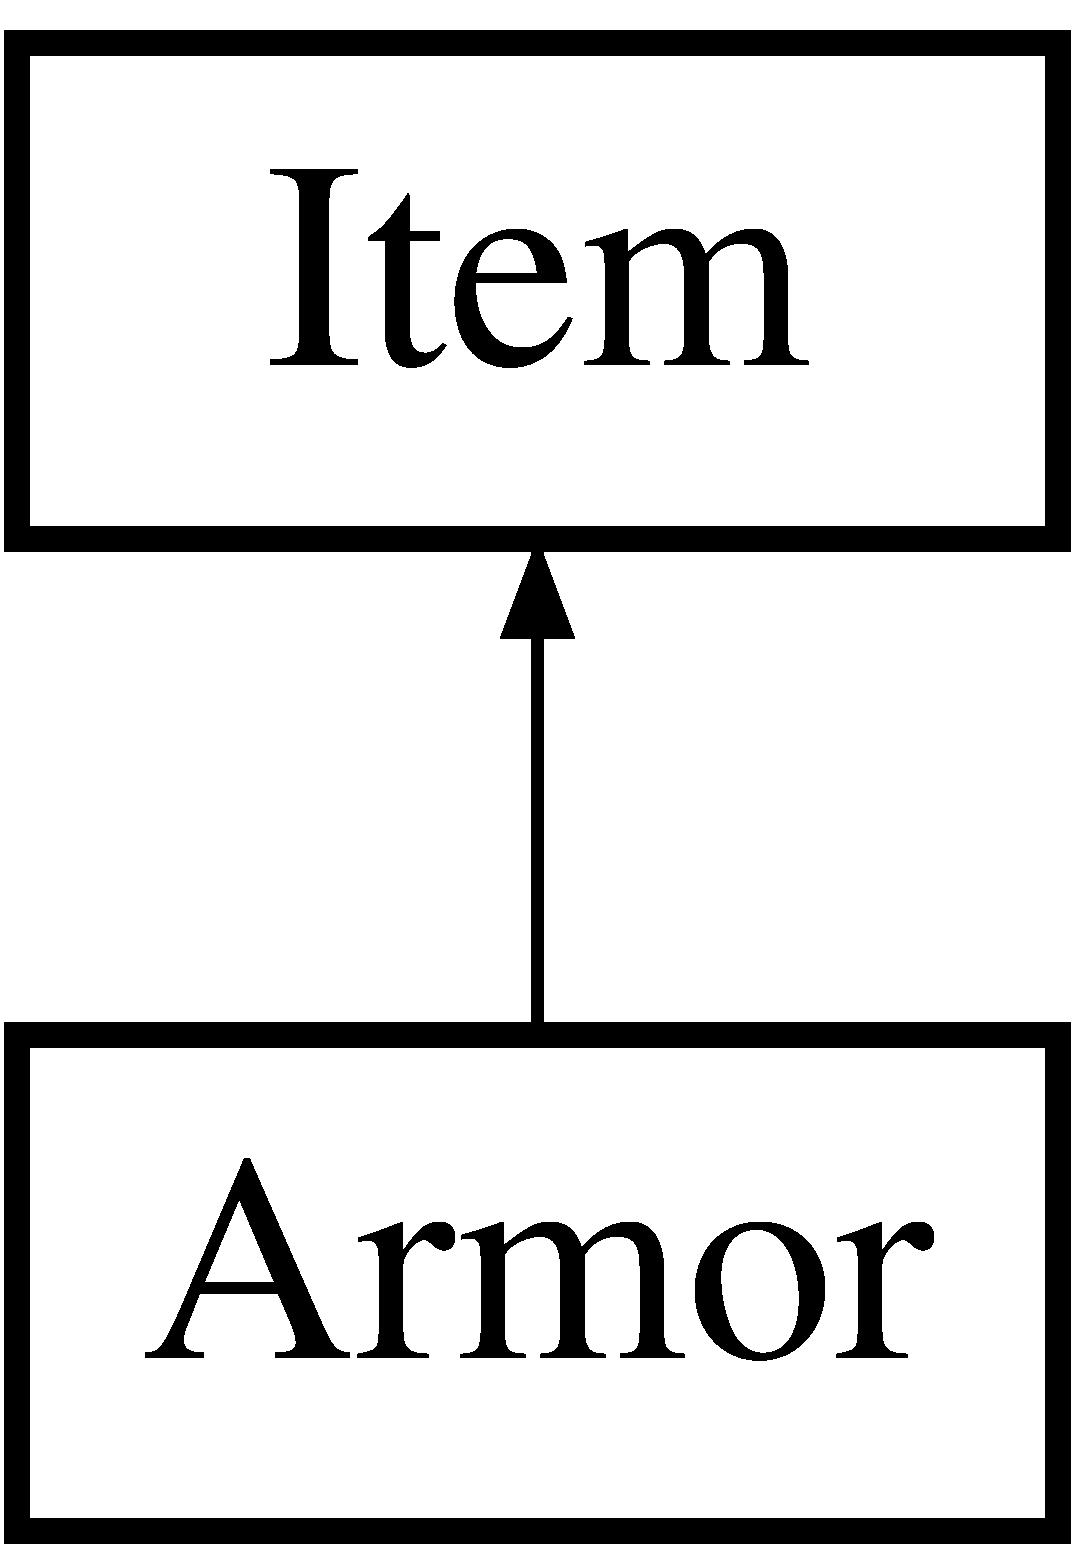
\includegraphics[height=2.000000cm]{class_armor}
\end{center}
\end{figure}
\subsection*{Public Member Functions}
\begin{DoxyCompactItemize}
\item 
\hypertarget{class_armor_a23323e95bbeb488eb6fe54cbd83d49a2}{}\label{class_armor_a23323e95bbeb488eb6fe54cbd83d49a2} 
\hyperlink{class_armor_a23323e95bbeb488eb6fe54cbd83d49a2}{Armor} ()
\begin{DoxyCompactList}\small\item\em Default constructor. \end{DoxyCompactList}\item 
\hyperlink{class_armor_a64d656ec063fbefab565d1115f725a93}{Armor} (string name, int armor\+Class)
\begin{DoxyCompactList}\small\item\em Constructor. \end{DoxyCompactList}\item 
\hyperlink{class_armor_a2911c5c6132e32d6de2693ffffb8fc76}{Armor} (string name, vector$<$ \hyperlink{class_enhancement}{Enhancement} $>$ enhancements)
\begin{DoxyCompactList}\small\item\em Constructor taking a vector of enhancements as parameter. \end{DoxyCompactList}\item 
bool \hyperlink{class_armor_a97b69f2691b172bd79e256a487a7f204}{validate\+Item} ()
\begin{DoxyCompactList}\small\item\em Overrided method to validate that the armor only enhances \textquotesingle{}A\+R\+M\+OR C\+L\+A\+SS\textquotesingle{} and verify that the bonus values are within \mbox{[}1..5\mbox{]}. \end{DoxyCompactList}\end{DoxyCompactItemize}
\subsection*{Friends}
\begin{DoxyCompactItemize}
\item 
\hypertarget{class_armor_ac98d07dd8f7b70e16ccb9a01abf56b9c}{}\label{class_armor_ac98d07dd8f7b70e16ccb9a01abf56b9c} 
class {\bfseries boost\+::serialization\+::access}
\end{DoxyCompactItemize}
\subsection*{Additional Inherited Members}


\subsection{Detailed Description}
Class for the implementation of an armor. 

\subsection{Constructor \& Destructor Documentation}
\hypertarget{class_armor_a64d656ec063fbefab565d1115f725a93}{}\label{class_armor_a64d656ec063fbefab565d1115f725a93} 
\index{Armor@{Armor}!Armor@{Armor}}
\index{Armor@{Armor}!Armor@{Armor}}
\subsubsection{\texorpdfstring{Armor()}{Armor()}\hspace{0.1cm}{\footnotesize\ttfamily [1/2]}}
{\footnotesize\ttfamily Armor\+::\+Armor (\begin{DoxyParamCaption}\item[{string}]{name,  }\item[{int}]{armor\+Class\+Bonus }\end{DoxyParamCaption})}



Constructor. 

Constructor that calls an \hyperlink{class_item}{Item} constructor 
\begin{DoxyParams}{Parameters}
{\em name} & \+: Name of the armor item \\
\hline
{\em armor\+Class\+Bonus} & \+: Integer representing the enhancement bonus for the stats \hyperlink{class_armor}{Armor} Class \\
\hline
\end{DoxyParams}
\hypertarget{class_armor_a2911c5c6132e32d6de2693ffffb8fc76}{}\label{class_armor_a2911c5c6132e32d6de2693ffffb8fc76} 
\index{Armor@{Armor}!Armor@{Armor}}
\index{Armor@{Armor}!Armor@{Armor}}
\subsubsection{\texorpdfstring{Armor()}{Armor()}\hspace{0.1cm}{\footnotesize\ttfamily [2/2]}}
{\footnotesize\ttfamily Armor\+::\+Armor (\begin{DoxyParamCaption}\item[{string}]{name,  }\item[{vector$<$ \hyperlink{class_enhancement}{Enhancement} $>$}]{enhancements }\end{DoxyParamCaption})}



Constructor taking a vector of enhancements as parameter. 

Constructor taking a vector of enhancements as parameter 
\begin{DoxyParams}{Parameters}
{\em name} & \+: Name of the armor item \\
\hline
{\em enhancements} & \+: Vector of enhancements \\
\hline
\end{DoxyParams}


\subsection{Member Function Documentation}
\hypertarget{class_armor_a97b69f2691b172bd79e256a487a7f204}{}\label{class_armor_a97b69f2691b172bd79e256a487a7f204} 
\index{Armor@{Armor}!validate\+Item@{validate\+Item}}
\index{validate\+Item@{validate\+Item}!Armor@{Armor}}
\subsubsection{\texorpdfstring{validate\+Item()}{validateItem()}}
{\footnotesize\ttfamily bool Armor\+::validate\+Item (\begin{DoxyParamCaption}{ }\end{DoxyParamCaption})\hspace{0.3cm}{\ttfamily [virtual]}}



Overrided method to validate that the armor only enhances \textquotesingle{}A\+R\+M\+OR C\+L\+A\+SS\textquotesingle{} and verify that the bonus values are within \mbox{[}1..5\mbox{]}. 

Overrided method to validate that the armor only enhances \textquotesingle{}A\+R\+M\+OR C\+L\+A\+SS\textquotesingle{} and verify that the bonus values are within \mbox{[}1..5\mbox{]} \begin{DoxyReturn}{Returns}
True if the enhancement list is valid according to the rules, false if not 
\end{DoxyReturn}


Reimplemented from \hyperlink{class_item_a6603371b60aaded48f697975c81fc25b}{Item}.



The documentation for this class was generated from the following files\+:\begin{DoxyCompactItemize}
\item 
\hyperlink{_armor_8h}{Armor.\+h}\item 
\hyperlink{_armor_8cpp}{Armor.\+cpp}\end{DoxyCompactItemize}

\hypertarget{class_belt}{}\section{Belt Class Reference}
\label{class_belt}\index{Belt@{Belt}}


Class for the implementation of a belt.  




{\ttfamily \#include $<$Belt.\+h$>$}

Inheritance diagram for Belt\+:\begin{figure}[H]
\begin{center}
\leavevmode
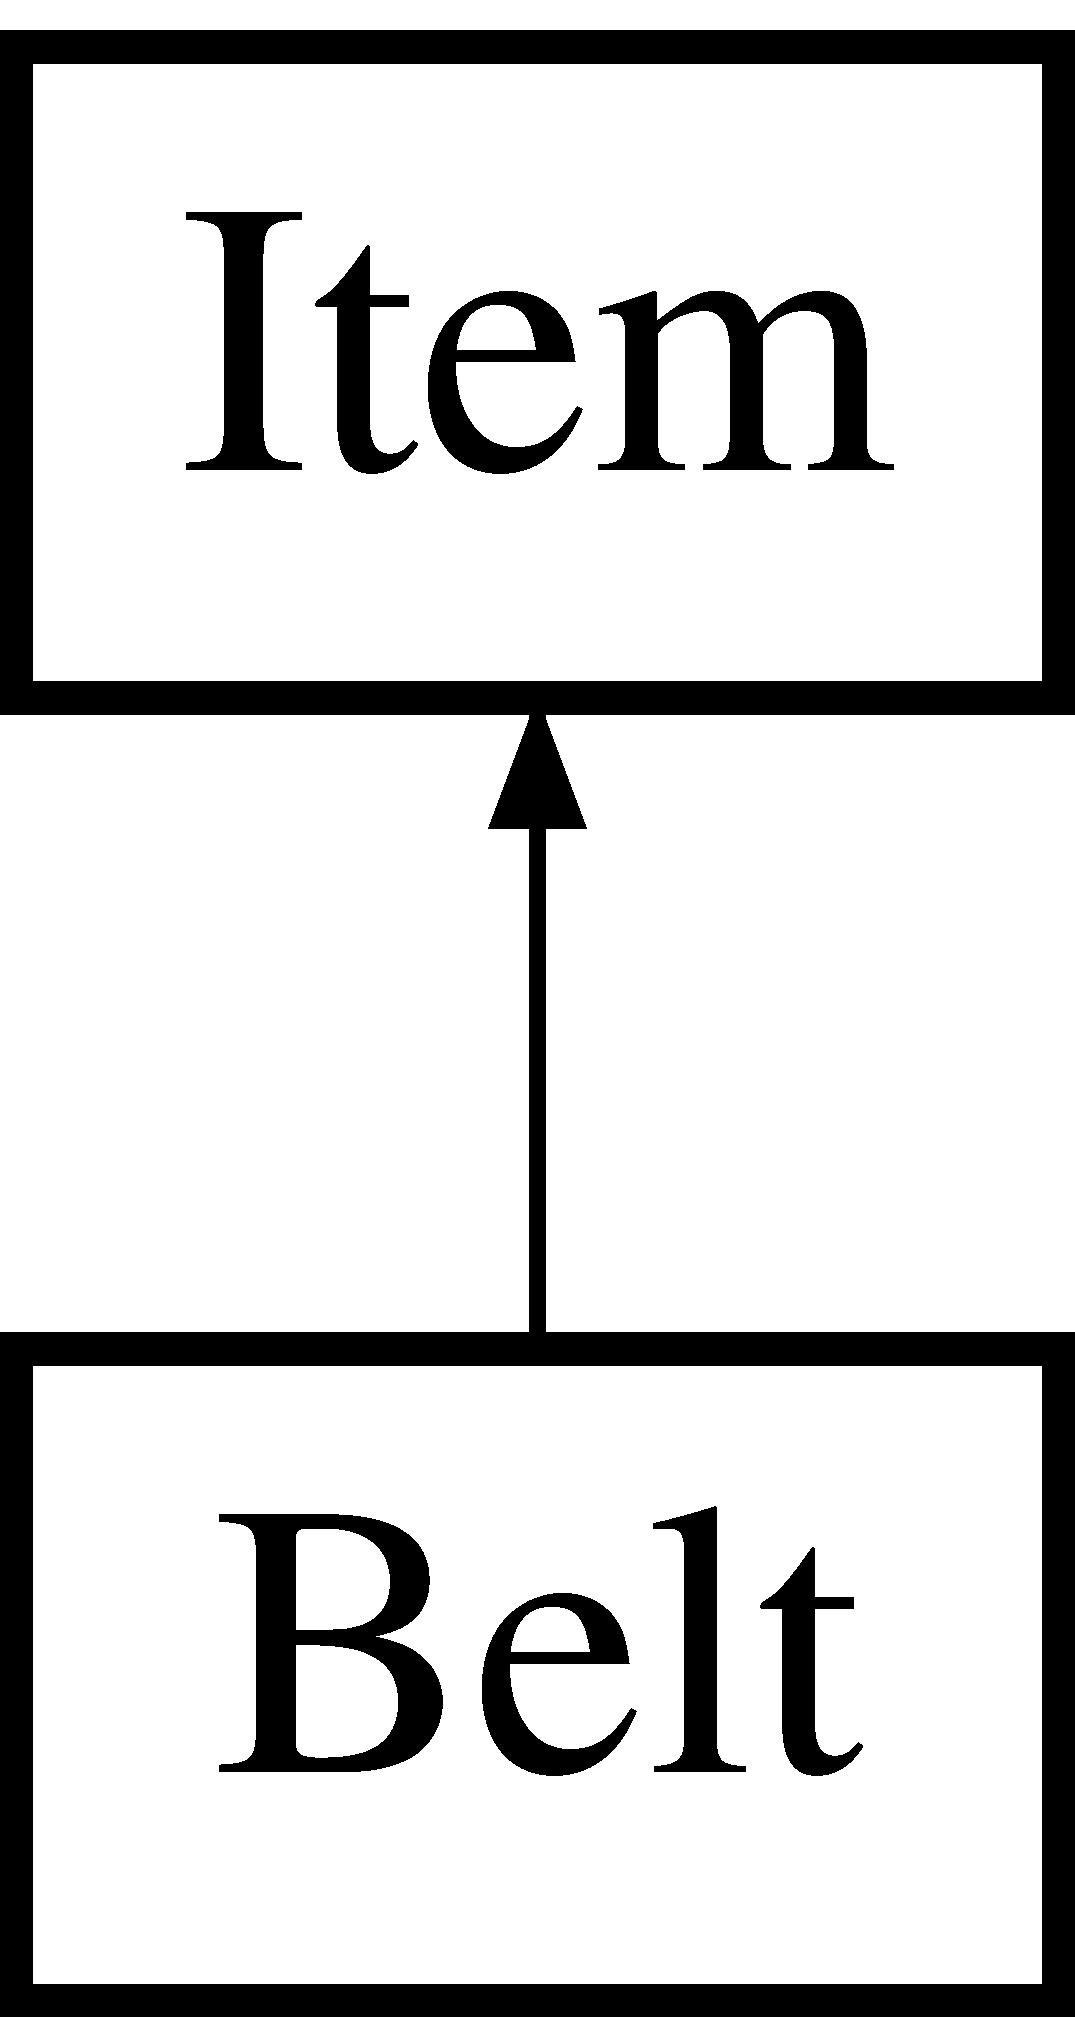
\includegraphics[height=2.000000cm]{class_belt}
\end{center}
\end{figure}
\subsection*{Public Member Functions}
\begin{DoxyCompactItemize}
\item 
\hypertarget{class_belt_a6dc40c21b5a62c71925df189511d7551}{}\label{class_belt_a6dc40c21b5a62c71925df189511d7551} 
\hyperlink{class_belt_a6dc40c21b5a62c71925df189511d7551}{Belt} ()
\begin{DoxyCompactList}\small\item\em Default constructor. \end{DoxyCompactList}\item 
\hyperlink{class_belt_ab54648057c8b264df3ffb71c4408a546}{Belt} (string name, int constitution, int strength)
\begin{DoxyCompactList}\small\item\em Constructor. \end{DoxyCompactList}\item 
\hyperlink{class_belt_aa29331f3e861aea90a39e5e723ccb562}{Belt} (string name, vector$<$ \hyperlink{class_enhancement}{Enhancement} $>$ enhancements)
\begin{DoxyCompactList}\small\item\em Constructor. \end{DoxyCompactList}\item 
bool \hyperlink{class_belt_ab374477dd9d966e6e6b81b3699afd939}{validate\+Item} ()
\begin{DoxyCompactList}\small\item\em Overrided method to validate that the armor only enhances \textquotesingle{}C\+O\+N\+S\+T\+I\+T\+U\+T\+I\+ON\textquotesingle{} and \textquotesingle{}S\+T\+R\+E\+N\+G\+TH\textquotesingle{} and verify that the bonus values are within \mbox{[}1..5\mbox{]}. \end{DoxyCompactList}\end{DoxyCompactItemize}
\subsection*{Friends}
\begin{DoxyCompactItemize}
\item 
\hypertarget{class_belt_ac98d07dd8f7b70e16ccb9a01abf56b9c}{}\label{class_belt_ac98d07dd8f7b70e16ccb9a01abf56b9c} 
class \hyperlink{class_belt_ac98d07dd8f7b70e16ccb9a01abf56b9c}{boost\+::serialization\+::access}
\begin{DoxyCompactList}\small\item\em serialization \end{DoxyCompactList}\end{DoxyCompactItemize}
\subsection*{Additional Inherited Members}


\subsection{Detailed Description}
Class for the implementation of a belt. 

\subsection{Constructor \& Destructor Documentation}
\hypertarget{class_belt_ab54648057c8b264df3ffb71c4408a546}{}\label{class_belt_ab54648057c8b264df3ffb71c4408a546} 
\index{Belt@{Belt}!Belt@{Belt}}
\index{Belt@{Belt}!Belt@{Belt}}
\subsubsection{\texorpdfstring{Belt()}{Belt()}\hspace{0.1cm}{\footnotesize\ttfamily [1/2]}}
{\footnotesize\ttfamily Belt\+::\+Belt (\begin{DoxyParamCaption}\item[{string}]{name,  }\item[{int}]{constitution\+Bonus,  }\item[{int}]{strength\+Bonus }\end{DoxyParamCaption})}



Constructor. 

Constructor that calls an \hyperlink{class_item}{Item} constructor 
\begin{DoxyParams}{Parameters}
{\em name} & \+: Name of the belt item \\
\hline
{\em constitution\+Bonus} & \+: Integer representing the enhancement bonus for the stats Constitution \\
\hline
{\em strength\+Bonus} & \+: Integer representing the enhancement bonus for the stats Strength \\
\hline
\end{DoxyParams}
\hypertarget{class_belt_aa29331f3e861aea90a39e5e723ccb562}{}\label{class_belt_aa29331f3e861aea90a39e5e723ccb562} 
\index{Belt@{Belt}!Belt@{Belt}}
\index{Belt@{Belt}!Belt@{Belt}}
\subsubsection{\texorpdfstring{Belt()}{Belt()}\hspace{0.1cm}{\footnotesize\ttfamily [2/2]}}
{\footnotesize\ttfamily Belt\+::\+Belt (\begin{DoxyParamCaption}\item[{string}]{name,  }\item[{vector$<$ \hyperlink{class_enhancement}{Enhancement} $>$}]{enhancements }\end{DoxyParamCaption})}



Constructor. 

Constructor taking a vector of enhancements as parameter It also calls an \hyperlink{class_item}{Item} constructor and pass a vector of enhancements as parameter. 
\begin{DoxyParams}{Parameters}
{\em name} & \+: Name of the belt item \\
\hline
{\em enhancements} & \+: Vector of enhancements \\
\hline
\end{DoxyParams}


\subsection{Member Function Documentation}
\hypertarget{class_belt_ab374477dd9d966e6e6b81b3699afd939}{}\label{class_belt_ab374477dd9d966e6e6b81b3699afd939} 
\index{Belt@{Belt}!validate\+Item@{validate\+Item}}
\index{validate\+Item@{validate\+Item}!Belt@{Belt}}
\subsubsection{\texorpdfstring{validate\+Item()}{validateItem()}}
{\footnotesize\ttfamily bool Belt\+::validate\+Item (\begin{DoxyParamCaption}{ }\end{DoxyParamCaption})\hspace{0.3cm}{\ttfamily [virtual]}}



Overrided method to validate that the armor only enhances \textquotesingle{}C\+O\+N\+S\+T\+I\+T\+U\+T\+I\+ON\textquotesingle{} and \textquotesingle{}S\+T\+R\+E\+N\+G\+TH\textquotesingle{} and verify that the bonus values are within \mbox{[}1..5\mbox{]}. 

Overrided method to validate that the armor only enhances \textquotesingle{}C\+O\+N\+S\+T\+I\+T\+U\+T\+I\+ON\textquotesingle{} and \textquotesingle{}S\+T\+R\+E\+N\+G\+TH\textquotesingle{} and verify that the bonus values are within \mbox{[}1..5\mbox{]} \begin{DoxyReturn}{Returns}
True if the enhancement list is valid according to the rules, false if not 
\end{DoxyReturn}


Reimplemented from \hyperlink{class_item_a6603371b60aaded48f697975c81fc25b}{Item}.



The documentation for this class was generated from the following files\+:\begin{DoxyCompactItemize}
\item 
\hyperlink{_belt_8h}{Belt.\+h}\item 
\hyperlink{_belt_8cpp}{Belt.\+cpp}\end{DoxyCompactItemize}

\hypertarget{class_boots}{}\section{Boots Class Reference}
\label{class_boots}\index{Boots@{Boots}}


Class for the implementation of a boot.  




{\ttfamily \#include $<$Boots.\+h$>$}

Inheritance diagram for Boots\+:\begin{figure}[H]
\begin{center}
\leavevmode
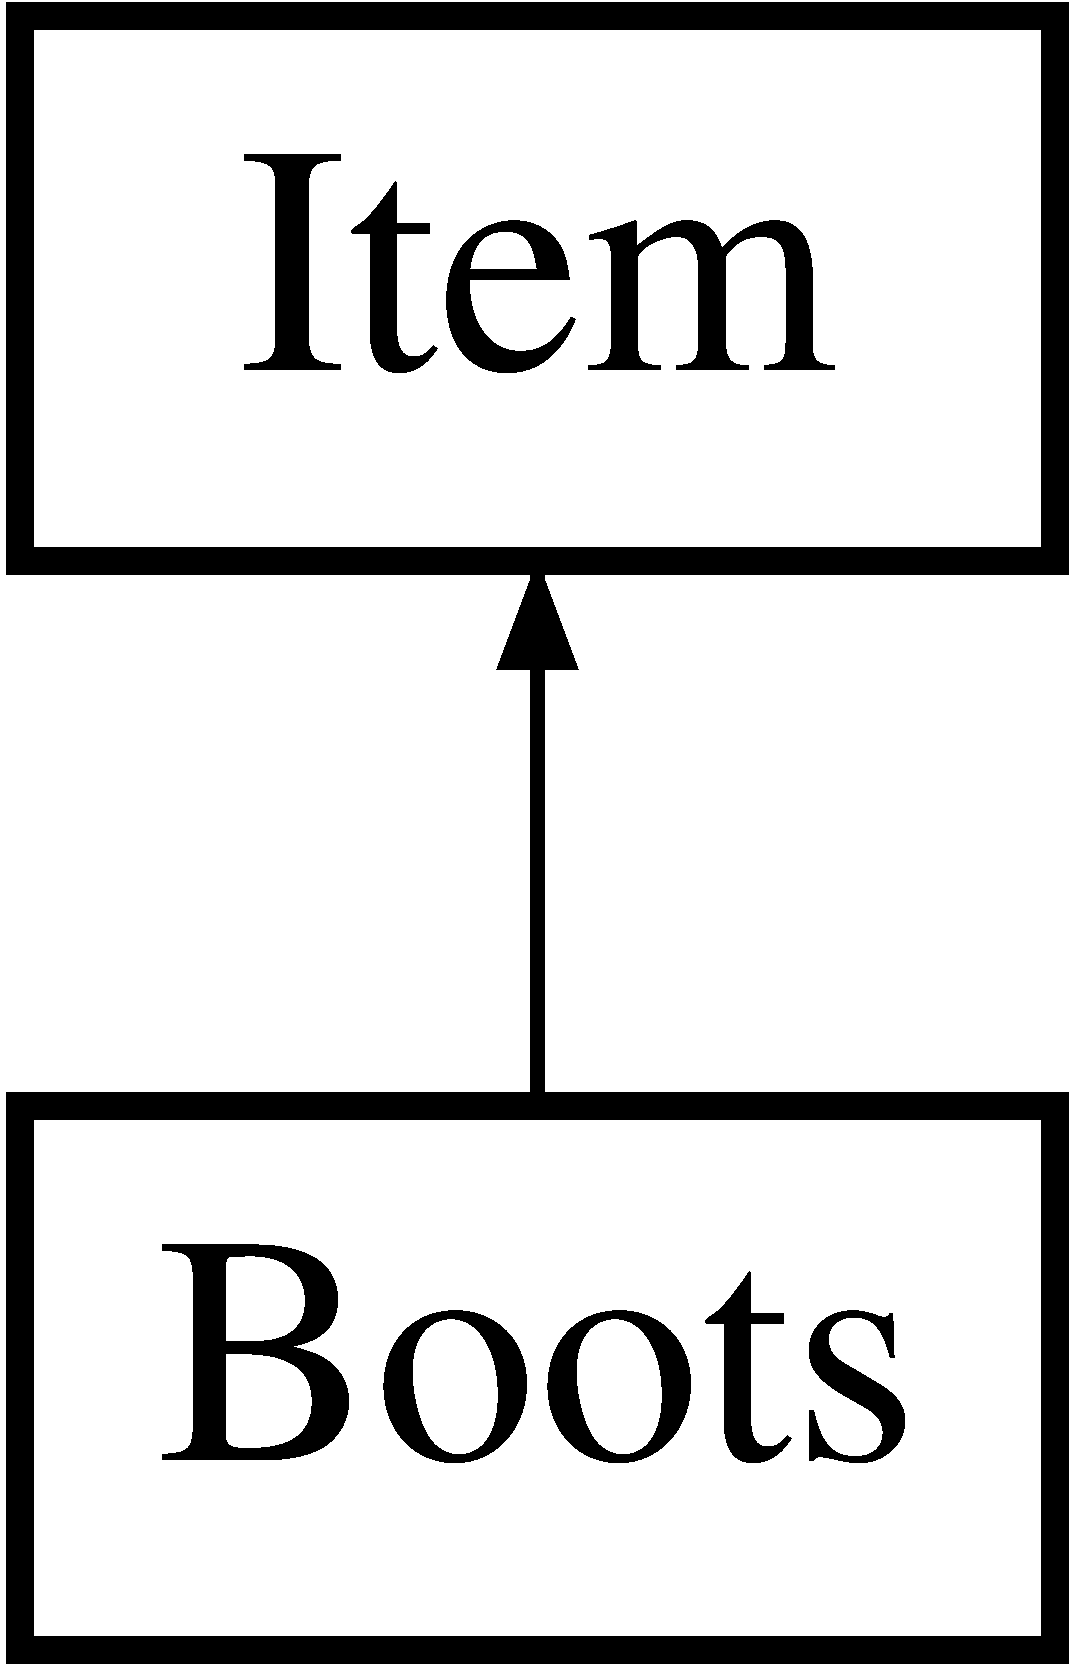
\includegraphics[height=2.000000cm]{class_boots}
\end{center}
\end{figure}
\subsection*{Public Member Functions}
\begin{DoxyCompactItemize}
\item 
\hypertarget{class_boots_abad208e963b53b1f29e269fc246a3485}{}\label{class_boots_abad208e963b53b1f29e269fc246a3485} 
\hyperlink{class_boots_abad208e963b53b1f29e269fc246a3485}{Boots} ()
\begin{DoxyCompactList}\small\item\em Default constructor. \end{DoxyCompactList}\item 
\hyperlink{class_boots_ab5fc35f0d1d71561bad9b81997cefc0f}{Boots} (string name, int armor\+Class, int dexterity)
\begin{DoxyCompactList}\small\item\em Constructor. \end{DoxyCompactList}\item 
\hyperlink{class_boots_a1cf3ea6e4ad15701b13f9010348a68d9}{Boots} (string name, vector$<$ \hyperlink{class_enhancement}{Enhancement} $>$ enhancements)
\begin{DoxyCompactList}\small\item\em Constructor taking a vector of enhancements as parameter. \end{DoxyCompactList}\item 
bool \hyperlink{class_boots_aac6123a5f117993f276eb5f2f343eeb0}{validate\+Item} ()
\begin{DoxyCompactList}\small\item\em Overrided method to validate that the armor only enhances \textquotesingle{}A\+R\+M\+OR C\+L\+A\+SS\textquotesingle{} and \textquotesingle{}D\+E\+X\+T\+E\+R\+I\+TY\textquotesingle{} and verify that the bonus values are within \mbox{[}1..5\mbox{]}. \end{DoxyCompactList}\end{DoxyCompactItemize}
\subsection*{Friends}
\begin{DoxyCompactItemize}
\item 
\hypertarget{class_boots_ac98d07dd8f7b70e16ccb9a01abf56b9c}{}\label{class_boots_ac98d07dd8f7b70e16ccb9a01abf56b9c} 
class \hyperlink{class_boots_ac98d07dd8f7b70e16ccb9a01abf56b9c}{boost\+::serialization\+::access}
\begin{DoxyCompactList}\small\item\em serialization \end{DoxyCompactList}\end{DoxyCompactItemize}
\subsection*{Additional Inherited Members}


\subsection{Detailed Description}
Class for the implementation of a boot. 

\subsection{Constructor \& Destructor Documentation}
\hypertarget{class_boots_ab5fc35f0d1d71561bad9b81997cefc0f}{}\label{class_boots_ab5fc35f0d1d71561bad9b81997cefc0f} 
\index{Boots@{Boots}!Boots@{Boots}}
\index{Boots@{Boots}!Boots@{Boots}}
\subsubsection{\texorpdfstring{Boots()}{Boots()}\hspace{0.1cm}{\footnotesize\ttfamily [1/2]}}
{\footnotesize\ttfamily Boots\+::\+Boots (\begin{DoxyParamCaption}\item[{string}]{name,  }\item[{int}]{armor\+Class\+Bonus,  }\item[{int}]{dexterity\+Bonus }\end{DoxyParamCaption})}



Constructor. 

Constructor that calls an \hyperlink{class_item}{Item} constructor 
\begin{DoxyParams}{Parameters}
{\em name} & \+: Name of the boots item \\
\hline
{\em armor\+Class\+Bonus} & \+: Integer representing the enhancement bonus for the stats \hyperlink{class_armor}{Armor} Class \\
\hline
{\em dexterity\+Bonus} & \+: Integer representing the enhancement bonus for the stats Dexterity \\
\hline
\end{DoxyParams}
\hypertarget{class_boots_a1cf3ea6e4ad15701b13f9010348a68d9}{}\label{class_boots_a1cf3ea6e4ad15701b13f9010348a68d9} 
\index{Boots@{Boots}!Boots@{Boots}}
\index{Boots@{Boots}!Boots@{Boots}}
\subsubsection{\texorpdfstring{Boots()}{Boots()}\hspace{0.1cm}{\footnotesize\ttfamily [2/2]}}
{\footnotesize\ttfamily Boots\+::\+Boots (\begin{DoxyParamCaption}\item[{string}]{name,  }\item[{vector$<$ \hyperlink{class_enhancement}{Enhancement} $>$}]{enhancements }\end{DoxyParamCaption})}



Constructor taking a vector of enhancements as parameter. 

Constructor taking a vector of enhancements as parameter 
\begin{DoxyParams}{Parameters}
{\em name} & \+: Name of the boots item \\
\hline
{\em enhancements} & \+: Vector of enhancements \\
\hline
\end{DoxyParams}


\subsection{Member Function Documentation}
\hypertarget{class_boots_aac6123a5f117993f276eb5f2f343eeb0}{}\label{class_boots_aac6123a5f117993f276eb5f2f343eeb0} 
\index{Boots@{Boots}!validate\+Item@{validate\+Item}}
\index{validate\+Item@{validate\+Item}!Boots@{Boots}}
\subsubsection{\texorpdfstring{validate\+Item()}{validateItem()}}
{\footnotesize\ttfamily bool Boots\+::validate\+Item (\begin{DoxyParamCaption}{ }\end{DoxyParamCaption})\hspace{0.3cm}{\ttfamily [virtual]}}



Overrided method to validate that the armor only enhances \textquotesingle{}A\+R\+M\+OR C\+L\+A\+SS\textquotesingle{} and \textquotesingle{}D\+E\+X\+T\+E\+R\+I\+TY\textquotesingle{} and verify that the bonus values are within \mbox{[}1..5\mbox{]}. 

Overrided method to validate that the armor only enhances \textquotesingle{}A\+R\+M\+OR C\+L\+A\+SS\textquotesingle{} and \textquotesingle{}D\+E\+X\+T\+E\+R\+I\+TY\textquotesingle{} and verify that the bonus values are within \mbox{[}1..5\mbox{]} \begin{DoxyReturn}{Returns}
True if the enhancement list is valid according to the rules, false if not 
\end{DoxyReturn}


Reimplemented from \hyperlink{class_item_a6603371b60aaded48f697975c81fc25b}{Item}.



The documentation for this class was generated from the following files\+:\begin{DoxyCompactItemize}
\item 
\hyperlink{_boots_8h}{Boots.\+h}\item 
\hyperlink{_boots_8cpp}{Boots.\+cpp}\end{DoxyCompactItemize}

\hypertarget{class_campaign}{}\section{Campaign Class Reference}
\label{class_campaign}\index{Campaign@{Campaign}}
\subsection*{Public Member Functions}
\begin{DoxyCompactItemize}
\item 
\hypertarget{class_campaign_ae81c5b000e416b0ef31994efdf871c40}{}\label{class_campaign_ae81c5b000e416b0ef31994efdf871c40} 
\hyperlink{class_campaign_ae81c5b000e416b0ef31994efdf871c40}{Campaign} ()
\begin{DoxyCompactList}\small\item\em Default constructor of campaign. \end{DoxyCompactList}\item 
void \hyperlink{class_campaign_a51ee2b7f2cb73b5e2ed75577d8d36ee2}{add\+Map} (string map\+Name)
\item 
\hypertarget{class_campaign_aa27fbd216917d08ceed2a05d791f7c6a}{}\label{class_campaign_aa27fbd216917d08ceed2a05d791f7c6a} 
void \hyperlink{class_campaign_aa27fbd216917d08ceed2a05d791f7c6a}{remove\+Map} ()
\begin{DoxyCompactList}\small\item\em Implementation of remove\+Map to remove the last map of the campaign in map\+Path\+List. \end{DoxyCompactList}\item 
string \hyperlink{class_campaign_a9813a6cab4db158847e83031db891b2a}{get\+Name} ()
\item 
\hypertarget{class_campaign_a9b8cd5a9a9f37f85b174c5beb5894fb6}{}\label{class_campaign_a9b8cd5a9a9f37f85b174c5beb5894fb6} 
void \hyperlink{class_campaign_a9b8cd5a9a9f37f85b174c5beb5894fb6}{set\+Name} (string name)
\begin{DoxyCompactList}\small\item\em Implementation of set\+Name to set the name of the campaign. \end{DoxyCompactList}\item 
int \hyperlink{class_campaign_a0eff36282a94a37fd5860550d9f2a217}{get\+Map\+List\+Size} ()
\item 
string \hyperlink{class_campaign_a1502a3bc96675f347158932960bbbb27}{get\+Map} (int index)
\item 
\hypertarget{class_campaign_a5cca9e21e4c057ffe862d1447f538e49}{}\label{class_campaign_a5cca9e21e4c057ffe862d1447f538e49} 
\hyperlink{class_campaign_a5cca9e21e4c057ffe862d1447f538e49}{$\sim$\+Campaign} ()
\begin{DoxyCompactList}\small\item\em Default destructor of class \hyperlink{class_campaign}{Campaign}. \end{DoxyCompactList}\end{DoxyCompactItemize}
\subsection*{Friends}
\begin{DoxyCompactItemize}
\item 
\hypertarget{class_campaign_ac98d07dd8f7b70e16ccb9a01abf56b9c}{}\label{class_campaign_ac98d07dd8f7b70e16ccb9a01abf56b9c} 
class \hyperlink{class_campaign_ac98d07dd8f7b70e16ccb9a01abf56b9c}{boost\+::serialization\+::access}
\begin{DoxyCompactList}\small\item\em Boost serialization. \end{DoxyCompactList}\end{DoxyCompactItemize}


\subsection{Member Function Documentation}
\hypertarget{class_campaign_a51ee2b7f2cb73b5e2ed75577d8d36ee2}{}\label{class_campaign_a51ee2b7f2cb73b5e2ed75577d8d36ee2} 
\index{Campaign@{Campaign}!add\+Map@{add\+Map}}
\index{add\+Map@{add\+Map}!Campaign@{Campaign}}
\subsubsection{\texorpdfstring{add\+Map()}{addMap()}}
{\footnotesize\ttfamily void Campaign\+::add\+Map (\begin{DoxyParamCaption}\item[{string}]{map\+Name }\end{DoxyParamCaption})}

Implementation of add\+Map to add a map to the map\+Path\+List 
\begin{DoxyParams}{Parameters}
{\em map\+Name} & \+: a string representing the name of the map to add \\
\hline
\end{DoxyParams}
\hypertarget{class_campaign_a1502a3bc96675f347158932960bbbb27}{}\label{class_campaign_a1502a3bc96675f347158932960bbbb27} 
\index{Campaign@{Campaign}!get\+Map@{get\+Map}}
\index{get\+Map@{get\+Map}!Campaign@{Campaign}}
\subsubsection{\texorpdfstring{get\+Map()}{getMap()}}
{\footnotesize\ttfamily string Campaign\+::get\+Map (\begin{DoxyParamCaption}\item[{int}]{index }\end{DoxyParamCaption})}

Implementation of get\+Map to return the name of the map at a specific index 
\begin{DoxyParams}{Parameters}
{\em index} & \+: integer value of the index to find the map \\
\hline
\end{DoxyParams}
\begin{DoxyReturn}{Returns}
\+: a string representating the specified map 
\end{DoxyReturn}
\hypertarget{class_campaign_a0eff36282a94a37fd5860550d9f2a217}{}\label{class_campaign_a0eff36282a94a37fd5860550d9f2a217} 
\index{Campaign@{Campaign}!get\+Map\+List\+Size@{get\+Map\+List\+Size}}
\index{get\+Map\+List\+Size@{get\+Map\+List\+Size}!Campaign@{Campaign}}
\subsubsection{\texorpdfstring{get\+Map\+List\+Size()}{getMapListSize()}}
{\footnotesize\ttfamily int Campaign\+::get\+Map\+List\+Size (\begin{DoxyParamCaption}{ }\end{DoxyParamCaption})}

Implementation of get\+Map\+List\+Size to return the size of the campaign \begin{DoxyReturn}{Returns}
\+: an integer value representing the size of the campaign 
\end{DoxyReturn}
\hypertarget{class_campaign_a9813a6cab4db158847e83031db891b2a}{}\label{class_campaign_a9813a6cab4db158847e83031db891b2a} 
\index{Campaign@{Campaign}!get\+Name@{get\+Name}}
\index{get\+Name@{get\+Name}!Campaign@{Campaign}}
\subsubsection{\texorpdfstring{get\+Name()}{getName()}}
{\footnotesize\ttfamily string Campaign\+::get\+Name (\begin{DoxyParamCaption}{ }\end{DoxyParamCaption})}

Implementation of get\+Name to return the name of the campaign \begin{DoxyReturn}{Returns}
\+: a string value representing the name of the campaign 
\end{DoxyReturn}


The documentation for this class was generated from the following files\+:\begin{DoxyCompactItemize}
\item 
\hyperlink{_campaign_8h}{Campaign.\+h}\item 
Campaign.\+cpp\end{DoxyCompactItemize}

\hypertarget{class_campaign_editor}{}\section{Campaign\+Editor Class Reference}
\label{class_campaign_editor}\index{Campaign\+Editor@{Campaign\+Editor}}
\subsection*{Public Member Functions}
\begin{DoxyCompactItemize}
\item 
\hypertarget{class_campaign_editor_a1f9e45e60a19fb2372d38a9a9f0dd745}{}\label{class_campaign_editor_a1f9e45e60a19fb2372d38a9a9f0dd745} 
\hyperlink{class_campaign_editor_a1f9e45e60a19fb2372d38a9a9f0dd745}{Campaign\+Editor} ()
\begin{DoxyCompactList}\small\item\em Implementation of the default constructor of \hyperlink{class_campaign_editor}{Campaign\+Editor}. \end{DoxyCompactList}\item 
\hypertarget{class_campaign_editor_a1d734e04cf258ab8b3d51f83f471334e}{}\label{class_campaign_editor_a1d734e04cf258ab8b3d51f83f471334e} 
void \hyperlink{class_campaign_editor_a1d734e04cf258ab8b3d51f83f471334e}{new\+Campaign} ()
\begin{DoxyCompactList}\small\item\em Implementation of new\+Campaign to create a new campaign. \end{DoxyCompactList}\item 
\hypertarget{class_campaign_editor_aeef9c6befce9bf6702c5118c1317feb0}{}\label{class_campaign_editor_aeef9c6befce9bf6702c5118c1317feb0} 
void \hyperlink{class_campaign_editor_aeef9c6befce9bf6702c5118c1317feb0}{set\+Available\+Maps} ()
\begin{DoxyCompactList}\small\item\em Implementation of set\+Available\+Maps to set all the available maps in the available\+Maps vector. \end{DoxyCompactList}\item 
\hypertarget{class_campaign_editor_a07ca1759b2e1b0a05566a19a73db26de}{}\label{class_campaign_editor_a07ca1759b2e1b0a05566a19a73db26de} 
void \hyperlink{class_campaign_editor_a07ca1759b2e1b0a05566a19a73db26de}{set\+Available\+Campaigns} ()
\begin{DoxyCompactList}\small\item\em Implementation of set\+Available\+Campaigns to set all the available campaigns in the available\+Campaigns vector. \end{DoxyCompactList}\item 
void \hyperlink{class_campaign_editor_af034142dc6af33969dd15788881ef238}{add\+Map} (string map\+Name)
\item 
\hypertarget{class_campaign_editor_aeb4ffe0a48aeaab7881beafb5dc03253}{}\label{class_campaign_editor_aeb4ffe0a48aeaab7881beafb5dc03253} 
void \hyperlink{class_campaign_editor_aeb4ffe0a48aeaab7881beafb5dc03253}{remove\+Map} ()
\begin{DoxyCompactList}\small\item\em Implementation of remove\+Map to remove the last map of the campaign. \end{DoxyCompactList}\item 
string \hyperlink{class_campaign_editor_a032797d696d1ef3e092756ea3fb6a8e8}{get\+Map} (int index)
\item 
string \hyperlink{class_campaign_editor_a08c98dcccedb2d109a3eca6ca47f7749}{get\+Available\+Map} (int index)
\item 
string \hyperlink{class_campaign_editor_aab2f6f1c0ae07f3ba60c6c23a85e77de}{get\+Available\+Campaigns} (int index)
\item 
int \hyperlink{class_campaign_editor_ae5046609eeca16a31392bcabcdb1db74}{get\+Available\+Maps\+Size} ()
\item 
\hypertarget{class_campaign_editor_a1f117cb0964d7ebc0b36fe6207d252c4}{}\label{class_campaign_editor_a1f117cb0964d7ebc0b36fe6207d252c4} 
int {\bfseries get\+Available\+Campaigns\+Size} ()
\item 
int \hyperlink{class_campaign_editor_afa6ea5f195b60ff60ceba7625e417613}{get\+Campaign\+Size} ()
\item 
\hypertarget{class_campaign_editor_a9ba86d9aac3530d9837aa739fb655a17}{}\label{class_campaign_editor_a9ba86d9aac3530d9837aa739fb655a17} 
bool \hyperlink{class_campaign_editor_a9ba86d9aac3530d9837aa739fb655a17}{load\+Maps} ()
\begin{DoxyCompactList}\small\item\em Implementation of load\+Maps to load all the maps of the campaign into campaign\+Maps. \end{DoxyCompactList}\item 
\hyperlink{class_map}{Map} $\ast$ \hyperlink{class_campaign_editor_a4524f058b13cb5ab04a65a04c7694550}{get\+Campaign\+Map} (int index)
\item 
bool \hyperlink{class_campaign_editor_ad27545a0bba9e86e5b03d20ca6e8d828}{load\+Campaign} (string campaign\+Name)
\item 
void \hyperlink{class_campaign_editor_a22419d5d2e5ef10d667523e9d113b5c2}{save\+Campaign} (string campaign\+Name)
\item 
\hypertarget{class_campaign_editor_a30a94a60280dfd225d6ec54dc0977b1e}{}\label{class_campaign_editor_a30a94a60280dfd225d6ec54dc0977b1e} 
\hyperlink{class_campaign_editor_a30a94a60280dfd225d6ec54dc0977b1e}{$\sim$\+Campaign\+Editor} ()
\begin{DoxyCompactList}\small\item\em Implementation of destructor of \hyperlink{class_campaign_editor}{Campaign\+Editor} class. \end{DoxyCompactList}\end{DoxyCompactItemize}


\subsection{Member Function Documentation}
\hypertarget{class_campaign_editor_af034142dc6af33969dd15788881ef238}{}\label{class_campaign_editor_af034142dc6af33969dd15788881ef238} 
\index{Campaign\+Editor@{Campaign\+Editor}!add\+Map@{add\+Map}}
\index{add\+Map@{add\+Map}!Campaign\+Editor@{Campaign\+Editor}}
\subsubsection{\texorpdfstring{add\+Map()}{addMap()}}
{\footnotesize\ttfamily void Campaign\+Editor\+::add\+Map (\begin{DoxyParamCaption}\item[{string}]{map\+Name }\end{DoxyParamCaption})}

Implementation of add\+Map to add a map in a campaign 
\begin{DoxyParams}{Parameters}
{\em map\+Name} & \+: a string value of the name of the map \\
\hline
\end{DoxyParams}
\hypertarget{class_campaign_editor_aab2f6f1c0ae07f3ba60c6c23a85e77de}{}\label{class_campaign_editor_aab2f6f1c0ae07f3ba60c6c23a85e77de} 
\index{Campaign\+Editor@{Campaign\+Editor}!get\+Available\+Campaigns@{get\+Available\+Campaigns}}
\index{get\+Available\+Campaigns@{get\+Available\+Campaigns}!Campaign\+Editor@{Campaign\+Editor}}
\subsubsection{\texorpdfstring{get\+Available\+Campaigns()}{getAvailableCampaigns()}}
{\footnotesize\ttfamily string Campaign\+Editor\+::get\+Available\+Campaigns (\begin{DoxyParamCaption}\item[{int}]{index }\end{DoxyParamCaption})}

Implementation of get\+Available\+Campaigns to get a specific saved campaign 
\begin{DoxyParams}{Parameters}
{\em index} & \+: an integer value of the position of the campaign in the vector \\
\hline
\end{DoxyParams}
\begin{DoxyReturn}{Returns}
\+: a string representing the name of the campaign 
\end{DoxyReturn}
\hypertarget{class_campaign_editor_a08c98dcccedb2d109a3eca6ca47f7749}{}\label{class_campaign_editor_a08c98dcccedb2d109a3eca6ca47f7749} 
\index{Campaign\+Editor@{Campaign\+Editor}!get\+Available\+Map@{get\+Available\+Map}}
\index{get\+Available\+Map@{get\+Available\+Map}!Campaign\+Editor@{Campaign\+Editor}}
\subsubsection{\texorpdfstring{get\+Available\+Map()}{getAvailableMap()}}
{\footnotesize\ttfamily string Campaign\+Editor\+::get\+Available\+Map (\begin{DoxyParamCaption}\item[{int}]{index }\end{DoxyParamCaption})}

Implementation of get\+Available\+Map to get a specific saved map 
\begin{DoxyParams}{Parameters}
{\em index} & \+: an integer value of the position of the map in the vector \\
\hline
\end{DoxyParams}
\begin{DoxyReturn}{Returns}
\+: a string representing the name of the map 
\end{DoxyReturn}
\hypertarget{class_campaign_editor_ae5046609eeca16a31392bcabcdb1db74}{}\label{class_campaign_editor_ae5046609eeca16a31392bcabcdb1db74} 
\index{Campaign\+Editor@{Campaign\+Editor}!get\+Available\+Maps\+Size@{get\+Available\+Maps\+Size}}
\index{get\+Available\+Maps\+Size@{get\+Available\+Maps\+Size}!Campaign\+Editor@{Campaign\+Editor}}
\subsubsection{\texorpdfstring{get\+Available\+Maps\+Size()}{getAvailableMapsSize()}}
{\footnotesize\ttfamily int Campaign\+Editor\+::get\+Available\+Maps\+Size (\begin{DoxyParamCaption}{ }\end{DoxyParamCaption})}

Implementation of get\+Available\+Maps\+Size to get the number of maps available \begin{DoxyReturn}{Returns}
\+: an integer representing the size of the map 
\end{DoxyReturn}
\hypertarget{class_campaign_editor_a4524f058b13cb5ab04a65a04c7694550}{}\label{class_campaign_editor_a4524f058b13cb5ab04a65a04c7694550} 
\index{Campaign\+Editor@{Campaign\+Editor}!get\+Campaign\+Map@{get\+Campaign\+Map}}
\index{get\+Campaign\+Map@{get\+Campaign\+Map}!Campaign\+Editor@{Campaign\+Editor}}
\subsubsection{\texorpdfstring{get\+Campaign\+Map()}{getCampaignMap()}}
{\footnotesize\ttfamily \hyperlink{class_map}{Map} $\ast$ Campaign\+Editor\+::get\+Campaign\+Map (\begin{DoxyParamCaption}\item[{int}]{index }\end{DoxyParamCaption})}

Implementation of get\+Campaign\+Map to get a specific map from a campaign 
\begin{DoxyParams}{Parameters}
{\em index} & \+: an integer value of the position of the map in the campaign vector \\
\hline
\end{DoxyParams}
\begin{DoxyReturn}{Returns}
\+: a map object at the specified position 
\end{DoxyReturn}
\hypertarget{class_campaign_editor_afa6ea5f195b60ff60ceba7625e417613}{}\label{class_campaign_editor_afa6ea5f195b60ff60ceba7625e417613} 
\index{Campaign\+Editor@{Campaign\+Editor}!get\+Campaign\+Size@{get\+Campaign\+Size}}
\index{get\+Campaign\+Size@{get\+Campaign\+Size}!Campaign\+Editor@{Campaign\+Editor}}
\subsubsection{\texorpdfstring{get\+Campaign\+Size()}{getCampaignSize()}}
{\footnotesize\ttfamily int Campaign\+Editor\+::get\+Campaign\+Size (\begin{DoxyParamCaption}{ }\end{DoxyParamCaption})}

Implementation of get\+Campaign\+Size to get the size of the campaign vector \begin{DoxyReturn}{Returns}
\+: the size of the campaign vector 
\end{DoxyReturn}
\hypertarget{class_campaign_editor_a032797d696d1ef3e092756ea3fb6a8e8}{}\label{class_campaign_editor_a032797d696d1ef3e092756ea3fb6a8e8} 
\index{Campaign\+Editor@{Campaign\+Editor}!get\+Map@{get\+Map}}
\index{get\+Map@{get\+Map}!Campaign\+Editor@{Campaign\+Editor}}
\subsubsection{\texorpdfstring{get\+Map()}{getMap()}}
{\footnotesize\ttfamily string Campaign\+Editor\+::get\+Map (\begin{DoxyParamCaption}\item[{int}]{index }\end{DoxyParamCaption})}

Implementation of get\+Map to get the name of a map of the campaign object 
\begin{DoxyParams}{Parameters}
{\em index} & \+: an integer value of the position of the map \\
\hline
\end{DoxyParams}
\begin{DoxyReturn}{Returns}
\+: string representating name of the map at the specified position 
\end{DoxyReturn}
\hypertarget{class_campaign_editor_ad27545a0bba9e86e5b03d20ca6e8d828}{}\label{class_campaign_editor_ad27545a0bba9e86e5b03d20ca6e8d828} 
\index{Campaign\+Editor@{Campaign\+Editor}!load\+Campaign@{load\+Campaign}}
\index{load\+Campaign@{load\+Campaign}!Campaign\+Editor@{Campaign\+Editor}}
\subsubsection{\texorpdfstring{load\+Campaign()}{loadCampaign()}}
{\footnotesize\ttfamily bool Campaign\+Editor\+::load\+Campaign (\begin{DoxyParamCaption}\item[{string}]{campaign\+Name }\end{DoxyParamCaption})}

Implementation of load\+Campaign to load the specified campaign into the campaign object  \+: a string value representing the name of the campaign \hypertarget{class_campaign_editor_a22419d5d2e5ef10d667523e9d113b5c2}{}\label{class_campaign_editor_a22419d5d2e5ef10d667523e9d113b5c2} 
\index{Campaign\+Editor@{Campaign\+Editor}!save\+Campaign@{save\+Campaign}}
\index{save\+Campaign@{save\+Campaign}!Campaign\+Editor@{Campaign\+Editor}}
\subsubsection{\texorpdfstring{save\+Campaign()}{saveCampaign()}}
{\footnotesize\ttfamily void Campaign\+Editor\+::save\+Campaign (\begin{DoxyParamCaption}\item[{string}]{campaign\+Name }\end{DoxyParamCaption})}

Implementation of save\+Campaign to save the campaign 
\begin{DoxyParams}{Parameters}
{\em camapign\+Name} & \+: string representing the file name of the campaign \\
\hline
\end{DoxyParams}


The documentation for this class was generated from the following files\+:\begin{DoxyCompactItemize}
\item 
\hyperlink{_campaign_editor_8h}{Campaign\+Editor.\+h}\item 
\hyperlink{_campaign_editor_8cpp}{Campaign\+Editor.\+cpp}\end{DoxyCompactItemize}

\hypertarget{class_character}{}\section{Character Class Reference}
\label{class_character}\index{Character@{Character}}


Class that implements a character.  




{\ttfamily \#include $<$Character.\+h$>$}

Inheritance diagram for Character\+:\begin{figure}[H]
\begin{center}
\leavevmode
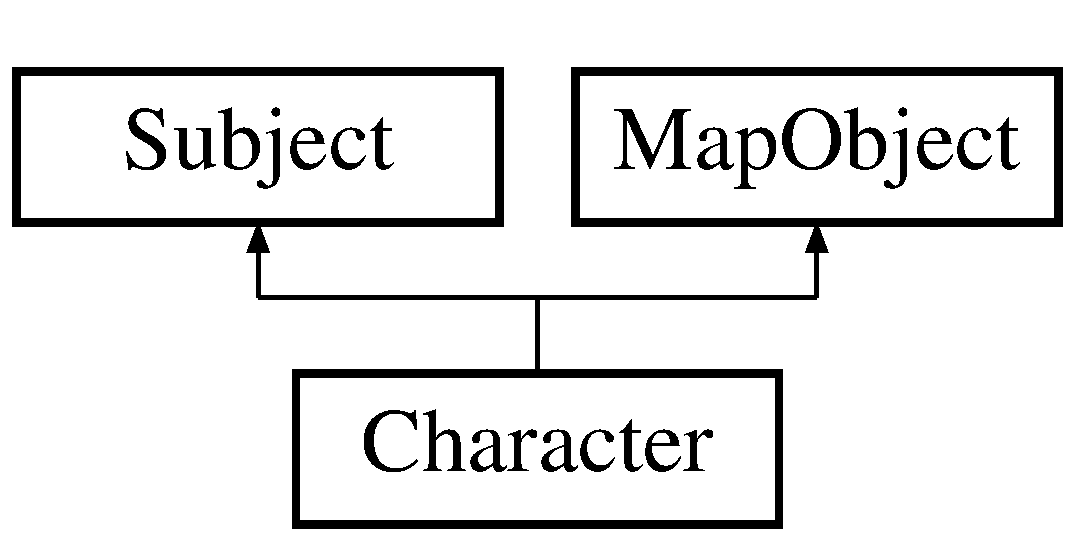
\includegraphics[height=2.000000cm]{class_character}
\end{center}
\end{figure}
\subsection*{Public Member Functions}
\begin{DoxyCompactItemize}
\item 
\hypertarget{class_character_adc27bdd255876169bad2ed0bae0cffb5}{}\label{class_character_adc27bdd255876169bad2ed0bae0cffb5} 
\hyperlink{class_character_adc27bdd255876169bad2ed0bae0cffb5}{Character} ()
\begin{DoxyCompactList}\small\item\em Default constructor for a fighter character. \end{DoxyCompactList}\item 
\hyperlink{class_character_aad0274b7a8cbb4fa8e0dddd0622d8870}{Character} (char, int, int, int, int, int, int)
\item 
\hypertarget{class_character_a9e9be564d05ded80962b2045aa70b3fc}{}\label{class_character_a9e9be564d05ded80962b2045aa70b3fc} 
\hyperlink{class_character_a9e9be564d05ded80962b2045aa70b3fc}{$\sim$\+Character} ()
\begin{DoxyCompactList}\small\item\em Destructor. \end{DoxyCompactList}\item 
bool \hyperlink{class_character_adae2bb0e0bb6b8d010be6d1ac3b1fd5f}{validate\+New\+Character} ()
\item 
void \hyperlink{class_character_a43566a6c7af77bde11b8f4c5e86c936f}{get\+Damaged} (int)
\item 
int \hyperlink{class_character_ac28870a30c9b451f55c3e27adaabfbfa}{get\+Hit\+Points} ()
\item 
int \hyperlink{class_character_a2c14caedf6a4a354589c14c7a2f53b0e}{get\+Max\+Hit\+Points} ()
\item 
int \hyperlink{class_character_a9710bee1a9f7c1e474abff5dd55adc8d}{roll\+Six\+Sided\+Die} ()
\item 
int \hyperlink{class_character_af3700e847620a19ada153eb10e600c22}{generate\+Ability\+Modifier} (int)
\item 
\hypertarget{class_character_a11166d1faa3af99548fa9e8dc2979eaf}{}\label{class_character_a11166d1faa3af99548fa9e8dc2979eaf} 
void \hyperlink{class_character_a11166d1faa3af99548fa9e8dc2979eaf}{calculate\+Ability\+Scores} (int\mbox{[}$\,$\mbox{]})
\begin{DoxyCompactList}\small\item\em Implementation of ability score calculator. \end{DoxyCompactList}\item 
void \hyperlink{class_character_a233f495f8092c80cf1951fd075e77ca7}{assign\+Ability\+Modifiers} (int\mbox{[}$\,$\mbox{]})
\item 
int \hyperlink{class_character_a6ab4e58439f6c394dc79f6a23440ef70}{roll\+Ten\+Sided\+Die} ()
\item 
\hypertarget{class_character_a0f993af09d2137001b12ab7b7415a55b}{}\label{class_character_a0f993af09d2137001b12ab7b7415a55b} 
void \hyperlink{class_character_a0f993af09d2137001b12ab7b7415a55b}{display\+Character\+Info} ()
\begin{DoxyCompactList}\small\item\em Method to display character information. \end{DoxyCompactList}\item 
int \hyperlink{class_character_aaaa0856b0bdcbc38c16ba5117df34ee8}{get\+Strength\+Score} ()
\item 
int \hyperlink{class_character_ac83cb6a4ea280a1e99418af81c4bae6c}{get\+Dexterity\+Score} ()
\item 
int \hyperlink{class_character_abbcc6a78fba81fa02add688b94c06376}{get\+Constitution\+Score} ()
\item 
int \hyperlink{class_character_a359c787d436784878e1f8650ddae3c35}{get\+Charisma\+Score} ()
\item 
int \hyperlink{class_character_a515aa3b9303281674dc82ad7d59e9337}{get\+Intelligence\+Score} ()
\item 
int \hyperlink{class_character_a07a2c6534ea013efc290aab432c11011}{get\+Wisdom\+Score} ()
\item 
int \hyperlink{class_character_aa0193d35d813ff170e5e3fbdcf259b8c}{get\+Strength\+Modifier} ()
\item 
int \hyperlink{class_character_ab4732b634d516b397142462b33e05782}{get\+Dexterity\+Modifier} ()
\item 
int \hyperlink{class_character_a61dd2cf1181a46ddecfdc8dede6fa732}{get\+Constitution\+Modifier} ()
\item 
int \hyperlink{class_character_a8b0adc0c65045b78e810fe436c636f4c}{get\+Charisma\+Modifier} ()
\item 
int \hyperlink{class_character_a562aa6723aba380cbddcf7467b921afb}{get\+Intelligence\+Modifier} ()
\item 
int \hyperlink{class_character_a860985777ed1f3f4bb5e4917f052afbd}{get\+Wisdom\+Modifier} ()
\item 
int \hyperlink{class_character_a9cf4ab6c7c066d38566773f946b64442}{get\+Current\+Level} ()
\item 
int \hyperlink{class_character_a79ce6ccb3e7d78ea75905d8d3f2ba4e2}{get\+Current\+Experience\+Points} ()
\item 
int \hyperlink{class_character_a10f27e812da8b25d4f44dbf6f3533fb2}{get\+Armor\+Class} ()
\item 
int \hyperlink{class_character_a94cb25ccbde6ccbc6aa6b3cca01dfebc}{get\+Attack\+Bonus} ()
\item 
int \hyperlink{class_character_a20ac6eab8a1df8ce849ad1015f656f96}{get\+Damage\+Bonus} ()
\item 
string \hyperlink{class_character_a3450bf341e820b6c14f3c3a2ebd7a3c3}{get\+Worn\+Item\+Name} (string)
\item 
void \hyperlink{class_character_a470a76c1062d97e40ce97997a4fdc62a}{set\+Level} (int)
\item 
void \hyperlink{class_character_a5a60696b6a658e78a08b3c098e1446d6}{set\+Current\+Hit\+Points} (int)
\item 
void \hyperlink{class_character_af277a2f17f94a7880af3204a4b824e06}{set\+Total\+Hit\+Points} (int)
\item 
void \hyperlink{class_character_a62ec21599695d548cada86de053dc51a}{set\+Strength\+Score} (int)
\item 
void \hyperlink{class_character_a6714e60888cf852dd48d45919c0e29c6}{set\+Dexterity\+Score} (int)
\item 
void \hyperlink{class_character_a959e82d760840d33ab95a264c549a8c6}{set\+Constitution\+Score} (int)
\item 
void \hyperlink{class_character_a7dff5255c010da8590f493078ab05db2}{set\+Charisma\+Score} (int)
\item 
void \hyperlink{class_character_a34f038f813b6b1522f41ba04f4620628}{set\+Intelligence\+Score} (int)
\item 
void \hyperlink{class_character_a9940a14b5050a9962ec6a042363a90d6}{set\+Wisdom\+Score} (int)
\item 
void \hyperlink{class_character_a543005270d3aa62d9aa0cb35aeac58b3}{set\+Strength\+Modifier} (int)
\item 
void \hyperlink{class_character_a667cb495021fa02cf0f0abebade3e3aa}{set\+Dexterity\+Modifier} (int)
\item 
void \hyperlink{class_character_ac550c6455f74ecbac744523fa82148c3}{set\+Constitution\+Modifier} (int)
\item 
void \hyperlink{class_character_a28ba83aeb0fae1450f69193001e433ec}{set\+Charisma\+Modifier} (int)
\item 
void \hyperlink{class_character_a554260d3ec37497bbdc7f1a22ddd7c78}{set\+Intelligence\+Modifier} (int)
\item 
void \hyperlink{class_character_af3e55f3f6018cf490471993ebcd95110}{set\+Wisdom\+Modifier} (int)
\item 
\hypertarget{class_character_aaaffb44b62eb70df0e545700c6011210}{}\label{class_character_aaaffb44b62eb70df0e545700c6011210} 
void \hyperlink{class_character_aaaffb44b62eb70df0e545700c6011210}{level\+Up} ()
\begin{DoxyCompactList}\small\item\em Method that increments the level by one to show that the character has leveled up. \end{DoxyCompactList}\item 
\hypertarget{class_character_a39139f003d8a88a27c8f91b0c0744834}{}\label{class_character_a39139f003d8a88a27c8f91b0c0744834} 
void \hyperlink{class_character_a39139f003d8a88a27c8f91b0c0744834}{display\+Equipment} ()
\begin{DoxyCompactList}\small\item\em Method that displays character\textquotesingle{}s current equipment. \end{DoxyCompactList}\item 
\hypertarget{class_character_a70de0e844848ee72cc7bb1c8dceef79c}{}\label{class_character_a70de0e844848ee72cc7bb1c8dceef79c} 
void \hyperlink{class_character_a70de0e844848ee72cc7bb1c8dceef79c}{display\+Backpack} ()
\begin{DoxyCompactList}\small\item\em Method that displays character\textquotesingle{}s inventory pane. \end{DoxyCompactList}\item 
bool \hyperlink{class_character_ae4953a40791d81dc7cab574aaeca7569}{validate\+Ability\+Modifiers} ()
\item 
void \hyperlink{class_character_af8a31bf573e0f2dc03e904165997bb21}{set\+Armor} (string)
\item 
void \hyperlink{class_character_af05444fdf239c036bf7cad6c5591419b}{set\+Shield} (string)
\item 
void \hyperlink{class_character_aaeee9a1f2678902c7749065a1bfabac9}{set\+Weapon} (string)
\item 
void \hyperlink{class_character_a611fea965a72947c1b53b79ee095f95e}{set\+Boots} (string)
\item 
void \hyperlink{class_character_a68653da50efcfeefca60d163bc30b419}{set\+Ring} (string)
\item 
void \hyperlink{class_character_a2e88779e8d7d6b1e9237c003b8b13d03}{set\+Helmet} (string)
\item 
\hypertarget{class_character_a7eba32ca277221f8804529722e9d939c}{}\label{class_character_a7eba32ca277221f8804529722e9d939c} 
void {\bfseries set\+Type} (char)
\item 
void \hyperlink{class_character_a2bbde472407d0c398cb602a45f5eec30}{equip\+Item} (int)
\item 
void \hyperlink{class_character_a9ee4f3f4e98b8babaa4d8e49ea44b99f}{unequip\+Item} (int)
\item 
int \hyperlink{class_character_ad47ab6e5a2671f770b5a580cb60baee7}{level\+Hit\+Points} ()
\item 
\hypertarget{class_character_a3a5ce729d6887d2c781cb5f246d122cb}{}\label{class_character_a3a5ce729d6887d2c781cb5f246d122cb} 
void {\bfseries choose\+Scores\+On\+Level\+Up} ()
\item 
\hypertarget{class_character_af23f19ad2075ea77bcd2f4e478cf0326}{}\label{class_character_af23f19ad2075ea77bcd2f4e478cf0326} 
string {\bfseries get\+Character\+Name} ()
\item 
\hypertarget{class_character_ae4c7d9343f6d25892a815e9301c0083d}{}\label{class_character_ae4c7d9343f6d25892a815e9301c0083d} 
void {\bfseries set\+Character\+Name} (string)
\item 
\hyperlink{class_item_container}{Item\+Container} $\ast$ \hyperlink{class_character_ad54a2ad63aa059d162cc67dbd0556f57}{get\+Equipped\+Items} ()
\item 
\hyperlink{class_item_container}{Item\+Container} $\ast$ \hyperlink{class_character_a92bf4b3daff50c95130f5727fd39a242}{get\+Backpack} ()
\end{DoxyCompactItemize}
\subsection*{Friends}
\begin{DoxyCompactItemize}
\item 
\hypertarget{class_character_ac98d07dd8f7b70e16ccb9a01abf56b9c}{}\label{class_character_ac98d07dd8f7b70e16ccb9a01abf56b9c} 
class {\bfseries boost\+::serialization\+::access}
\end{DoxyCompactItemize}
\subsection*{Additional Inherited Members}


\subsection{Detailed Description}
Class that implements a character. 

\subsection{Constructor \& Destructor Documentation}
\hypertarget{class_character_aad0274b7a8cbb4fa8e0dddd0622d8870}{}\label{class_character_aad0274b7a8cbb4fa8e0dddd0622d8870} 
\index{Character@{Character}!Character@{Character}}
\index{Character@{Character}!Character@{Character}}
\subsubsection{\texorpdfstring{Character()}{Character()}}
{\footnotesize\ttfamily Character\+::\+Character (\begin{DoxyParamCaption}\item[{char}]{type,  }\item[{int}]{str,  }\item[{int}]{dex,  }\item[{int}]{con,  }\item[{int}]{intel,  }\item[{int}]{wis,  }\item[{int}]{cha }\end{DoxyParamCaption})}

Constructor\+: Passes values to each ability score 
\begin{DoxyParams}{Parameters}
{\em str} & strength score, dex\+: dexterity score, con\+: constitution score, intel\+: intelligence score, wis\+: wisdom score, cha\+: charisma score \\
\hline
\end{DoxyParams}


\subsection{Member Function Documentation}
\hypertarget{class_character_a233f495f8092c80cf1951fd075e77ca7}{}\label{class_character_a233f495f8092c80cf1951fd075e77ca7} 
\index{Character@{Character}!assign\+Ability\+Modifiers@{assign\+Ability\+Modifiers}}
\index{assign\+Ability\+Modifiers@{assign\+Ability\+Modifiers}!Character@{Character}}
\subsubsection{\texorpdfstring{assign\+Ability\+Modifiers()}{assignAbilityModifiers()}}
{\footnotesize\ttfamily void Character\+::assign\+Ability\+Modifiers (\begin{DoxyParamCaption}\item[{int}]{holder\mbox{[}$\,$\mbox{]} }\end{DoxyParamCaption})}

Method to assign ability modifiers to the modifiers array 
\begin{DoxyParams}{Parameters}
{\em holder} & array that will be passed in this function \\
\hline
\end{DoxyParams}
\hypertarget{class_character_a2bbde472407d0c398cb602a45f5eec30}{}\label{class_character_a2bbde472407d0c398cb602a45f5eec30} 
\index{Character@{Character}!equip\+Item@{equip\+Item}}
\index{equip\+Item@{equip\+Item}!Character@{Character}}
\subsubsection{\texorpdfstring{equip\+Item()}{equipItem()}}
{\footnotesize\ttfamily void Character\+::equip\+Item (\begin{DoxyParamCaption}\item[{int}]{index }\end{DoxyParamCaption})}

Method to equip an item on the character from the backpack 
\begin{DoxyParams}{Parameters}
{\em } & The index position of the item to wear inside the vector representing a backpack \\
\hline
\end{DoxyParams}
\hypertarget{class_character_af3700e847620a19ada153eb10e600c22}{}\label{class_character_af3700e847620a19ada153eb10e600c22} 
\index{Character@{Character}!generate\+Ability\+Modifier@{generate\+Ability\+Modifier}}
\index{generate\+Ability\+Modifier@{generate\+Ability\+Modifier}!Character@{Character}}
\subsubsection{\texorpdfstring{generate\+Ability\+Modifier()}{generateAbilityModifier()}}
{\footnotesize\ttfamily int Character\+::generate\+Ability\+Modifier (\begin{DoxyParamCaption}\item[{int}]{score }\end{DoxyParamCaption})}

Implementation for an ability modifier calculator 
\begin{DoxyParams}{Parameters}
{\em score} & ability score for the certain attribute \\
\hline
\end{DoxyParams}
\begin{DoxyReturn}{Returns}
int value, the value of the corresponding ability modifier 
\end{DoxyReturn}
\hypertarget{class_character_a10f27e812da8b25d4f44dbf6f3533fb2}{}\label{class_character_a10f27e812da8b25d4f44dbf6f3533fb2} 
\index{Character@{Character}!get\+Armor\+Class@{get\+Armor\+Class}}
\index{get\+Armor\+Class@{get\+Armor\+Class}!Character@{Character}}
\subsubsection{\texorpdfstring{get\+Armor\+Class()}{getArmorClass()}}
{\footnotesize\ttfamily int Character\+::get\+Armor\+Class (\begin{DoxyParamCaption}{ }\end{DoxyParamCaption})}

Accessor method for character\textquotesingle{}s armor class \begin{DoxyReturn}{Returns}
int value, the value of the character\textquotesingle{}s armor class 
\end{DoxyReturn}
\hypertarget{class_character_a94cb25ccbde6ccbc6aa6b3cca01dfebc}{}\label{class_character_a94cb25ccbde6ccbc6aa6b3cca01dfebc} 
\index{Character@{Character}!get\+Attack\+Bonus@{get\+Attack\+Bonus}}
\index{get\+Attack\+Bonus@{get\+Attack\+Bonus}!Character@{Character}}
\subsubsection{\texorpdfstring{get\+Attack\+Bonus()}{getAttackBonus()}}
{\footnotesize\ttfamily int Character\+::get\+Attack\+Bonus (\begin{DoxyParamCaption}{ }\end{DoxyParamCaption})}

Accessor method for attack bonus \begin{DoxyReturn}{Returns}
int value\+: the value of the character\textquotesingle{}s attack bonus 
\end{DoxyReturn}
\hypertarget{class_character_a92bf4b3daff50c95130f5727fd39a242}{}\label{class_character_a92bf4b3daff50c95130f5727fd39a242} 
\index{Character@{Character}!get\+Backpack@{get\+Backpack}}
\index{get\+Backpack@{get\+Backpack}!Character@{Character}}
\subsubsection{\texorpdfstring{get\+Backpack()}{getBackpack()}}
{\footnotesize\ttfamily \hyperlink{class_item_container}{Item\+Container} $\ast$ Character\+::get\+Backpack (\begin{DoxyParamCaption}{ }\end{DoxyParamCaption})}

Method to get all items inside the backpack \begin{DoxyReturn}{Returns}
A pointer to an item container representing the backpack 
\end{DoxyReturn}
\hypertarget{class_character_a8b0adc0c65045b78e810fe436c636f4c}{}\label{class_character_a8b0adc0c65045b78e810fe436c636f4c} 
\index{Character@{Character}!get\+Charisma\+Modifier@{get\+Charisma\+Modifier}}
\index{get\+Charisma\+Modifier@{get\+Charisma\+Modifier}!Character@{Character}}
\subsubsection{\texorpdfstring{get\+Charisma\+Modifier()}{getCharismaModifier()}}
{\footnotesize\ttfamily int Character\+::get\+Charisma\+Modifier (\begin{DoxyParamCaption}{ }\end{DoxyParamCaption})}

Accessor method for charisma score modifier \begin{DoxyReturn}{Returns}
int value, the value of the charisma modifier 
\end{DoxyReturn}
\hypertarget{class_character_a359c787d436784878e1f8650ddae3c35}{}\label{class_character_a359c787d436784878e1f8650ddae3c35} 
\index{Character@{Character}!get\+Charisma\+Score@{get\+Charisma\+Score}}
\index{get\+Charisma\+Score@{get\+Charisma\+Score}!Character@{Character}}
\subsubsection{\texorpdfstring{get\+Charisma\+Score()}{getCharismaScore()}}
{\footnotesize\ttfamily int Character\+::get\+Charisma\+Score (\begin{DoxyParamCaption}{ }\end{DoxyParamCaption})}

Accessor method for charisma score attribute \begin{DoxyReturn}{Returns}
int value\+: the value of the charisma ability score 
\end{DoxyReturn}
\hypertarget{class_character_a61dd2cf1181a46ddecfdc8dede6fa732}{}\label{class_character_a61dd2cf1181a46ddecfdc8dede6fa732} 
\index{Character@{Character}!get\+Constitution\+Modifier@{get\+Constitution\+Modifier}}
\index{get\+Constitution\+Modifier@{get\+Constitution\+Modifier}!Character@{Character}}
\subsubsection{\texorpdfstring{get\+Constitution\+Modifier()}{getConstitutionModifier()}}
{\footnotesize\ttfamily int Character\+::get\+Constitution\+Modifier (\begin{DoxyParamCaption}{ }\end{DoxyParamCaption})}

Accessor method for constitution score modifier \begin{DoxyReturn}{Returns}
int value, the value of the constitution modifier 
\end{DoxyReturn}
\hypertarget{class_character_abbcc6a78fba81fa02add688b94c06376}{}\label{class_character_abbcc6a78fba81fa02add688b94c06376} 
\index{Character@{Character}!get\+Constitution\+Score@{get\+Constitution\+Score}}
\index{get\+Constitution\+Score@{get\+Constitution\+Score}!Character@{Character}}
\subsubsection{\texorpdfstring{get\+Constitution\+Score()}{getConstitutionScore()}}
{\footnotesize\ttfamily int Character\+::get\+Constitution\+Score (\begin{DoxyParamCaption}{ }\end{DoxyParamCaption})}

Accessor method for constitution score attribute \begin{DoxyReturn}{Returns}
int value, the value of the constitution ability score 
\end{DoxyReturn}
\hypertarget{class_character_a79ce6ccb3e7d78ea75905d8d3f2ba4e2}{}\label{class_character_a79ce6ccb3e7d78ea75905d8d3f2ba4e2} 
\index{Character@{Character}!get\+Current\+Experience\+Points@{get\+Current\+Experience\+Points}}
\index{get\+Current\+Experience\+Points@{get\+Current\+Experience\+Points}!Character@{Character}}
\subsubsection{\texorpdfstring{get\+Current\+Experience\+Points()}{getCurrentExperiencePoints()}}
{\footnotesize\ttfamily int Character\+::get\+Current\+Experience\+Points (\begin{DoxyParamCaption}{ }\end{DoxyParamCaption})}

Accessor method for experience points \begin{DoxyReturn}{Returns}
int value, the value of character\textquotesingle{}s current experience points 
\end{DoxyReturn}
\hypertarget{class_character_a9cf4ab6c7c066d38566773f946b64442}{}\label{class_character_a9cf4ab6c7c066d38566773f946b64442} 
\index{Character@{Character}!get\+Current\+Level@{get\+Current\+Level}}
\index{get\+Current\+Level@{get\+Current\+Level}!Character@{Character}}
\subsubsection{\texorpdfstring{get\+Current\+Level()}{getCurrentLevel()}}
{\footnotesize\ttfamily int Character\+::get\+Current\+Level (\begin{DoxyParamCaption}{ }\end{DoxyParamCaption})}

Accessor method for character\textquotesingle{}s current level \begin{DoxyReturn}{Returns}
int value, the value of the character\textquotesingle{}s level 
\end{DoxyReturn}
\hypertarget{class_character_a20ac6eab8a1df8ce849ad1015f656f96}{}\label{class_character_a20ac6eab8a1df8ce849ad1015f656f96} 
\index{Character@{Character}!get\+Damage\+Bonus@{get\+Damage\+Bonus}}
\index{get\+Damage\+Bonus@{get\+Damage\+Bonus}!Character@{Character}}
\subsubsection{\texorpdfstring{get\+Damage\+Bonus()}{getDamageBonus()}}
{\footnotesize\ttfamily int Character\+::get\+Damage\+Bonus (\begin{DoxyParamCaption}{ }\end{DoxyParamCaption})}

Accessor method for damage bonus \begin{DoxyReturn}{Returns}
int value, the value of the character\textquotesingle{}s damage bonus 
\end{DoxyReturn}
\hypertarget{class_character_a43566a6c7af77bde11b8f4c5e86c936f}{}\label{class_character_a43566a6c7af77bde11b8f4c5e86c936f} 
\index{Character@{Character}!get\+Damaged@{get\+Damaged}}
\index{get\+Damaged@{get\+Damaged}!Character@{Character}}
\subsubsection{\texorpdfstring{get\+Damaged()}{getDamaged()}}
{\footnotesize\ttfamily void Character\+::get\+Damaged (\begin{DoxyParamCaption}\item[{int}]{damage }\end{DoxyParamCaption})}

Method to get the damage received by the character Notify message is sent in this function in order to trigger an update of the view 
\begin{DoxyParams}{Parameters}
{\em damage} & damage sustained by the character \\
\hline
\end{DoxyParams}
\hypertarget{class_character_ab4732b634d516b397142462b33e05782}{}\label{class_character_ab4732b634d516b397142462b33e05782} 
\index{Character@{Character}!get\+Dexterity\+Modifier@{get\+Dexterity\+Modifier}}
\index{get\+Dexterity\+Modifier@{get\+Dexterity\+Modifier}!Character@{Character}}
\subsubsection{\texorpdfstring{get\+Dexterity\+Modifier()}{getDexterityModifier()}}
{\footnotesize\ttfamily int Character\+::get\+Dexterity\+Modifier (\begin{DoxyParamCaption}{ }\end{DoxyParamCaption})}

Accessor method for dexterity score modifier \begin{DoxyReturn}{Returns}
int value, the value of the dexterity modifier 
\end{DoxyReturn}
\hypertarget{class_character_ac83cb6a4ea280a1e99418af81c4bae6c}{}\label{class_character_ac83cb6a4ea280a1e99418af81c4bae6c} 
\index{Character@{Character}!get\+Dexterity\+Score@{get\+Dexterity\+Score}}
\index{get\+Dexterity\+Score@{get\+Dexterity\+Score}!Character@{Character}}
\subsubsection{\texorpdfstring{get\+Dexterity\+Score()}{getDexterityScore()}}
{\footnotesize\ttfamily int Character\+::get\+Dexterity\+Score (\begin{DoxyParamCaption}{ }\end{DoxyParamCaption})}

Accessor method for dexterity score attribute \begin{DoxyReturn}{Returns}
int value, the value of the dexterity ability score 
\end{DoxyReturn}
\hypertarget{class_character_ad54a2ad63aa059d162cc67dbd0556f57}{}\label{class_character_ad54a2ad63aa059d162cc67dbd0556f57} 
\index{Character@{Character}!get\+Equipped\+Items@{get\+Equipped\+Items}}
\index{get\+Equipped\+Items@{get\+Equipped\+Items}!Character@{Character}}
\subsubsection{\texorpdfstring{get\+Equipped\+Items()}{getEquippedItems()}}
{\footnotesize\ttfamily \hyperlink{class_item_container}{Item\+Container} $\ast$ Character\+::get\+Equipped\+Items (\begin{DoxyParamCaption}{ }\end{DoxyParamCaption})}

Method to get all equipped items \begin{DoxyReturn}{Returns}
A pointer to an item container representing equipped items 
\end{DoxyReturn}
\hypertarget{class_character_ac28870a30c9b451f55c3e27adaabfbfa}{}\label{class_character_ac28870a30c9b451f55c3e27adaabfbfa} 
\index{Character@{Character}!get\+Hit\+Points@{get\+Hit\+Points}}
\index{get\+Hit\+Points@{get\+Hit\+Points}!Character@{Character}}
\subsubsection{\texorpdfstring{get\+Hit\+Points()}{getHitPoints()}}
{\footnotesize\ttfamily int Character\+::get\+Hit\+Points (\begin{DoxyParamCaption}{ }\end{DoxyParamCaption})}

Method to get the current hit points \begin{DoxyReturn}{Returns}
int, value of current\+Hit\+Points 
\end{DoxyReturn}
\hypertarget{class_character_a562aa6723aba380cbddcf7467b921afb}{}\label{class_character_a562aa6723aba380cbddcf7467b921afb} 
\index{Character@{Character}!get\+Intelligence\+Modifier@{get\+Intelligence\+Modifier}}
\index{get\+Intelligence\+Modifier@{get\+Intelligence\+Modifier}!Character@{Character}}
\subsubsection{\texorpdfstring{get\+Intelligence\+Modifier()}{getIntelligenceModifier()}}
{\footnotesize\ttfamily int Character\+::get\+Intelligence\+Modifier (\begin{DoxyParamCaption}{ }\end{DoxyParamCaption})}

Accessor method for intelligence score modifier \begin{DoxyReturn}{Returns}
int value, the value of the intelligence modifier 
\end{DoxyReturn}
\hypertarget{class_character_a515aa3b9303281674dc82ad7d59e9337}{}\label{class_character_a515aa3b9303281674dc82ad7d59e9337} 
\index{Character@{Character}!get\+Intelligence\+Score@{get\+Intelligence\+Score}}
\index{get\+Intelligence\+Score@{get\+Intelligence\+Score}!Character@{Character}}
\subsubsection{\texorpdfstring{get\+Intelligence\+Score()}{getIntelligenceScore()}}
{\footnotesize\ttfamily int Character\+::get\+Intelligence\+Score (\begin{DoxyParamCaption}{ }\end{DoxyParamCaption})}

Accessor method for intelligence score attribute \begin{DoxyReturn}{Returns}
int value, the value of the intelligence ability score 
\end{DoxyReturn}
\hypertarget{class_character_a2c14caedf6a4a354589c14c7a2f53b0e}{}\label{class_character_a2c14caedf6a4a354589c14c7a2f53b0e} 
\index{Character@{Character}!get\+Max\+Hit\+Points@{get\+Max\+Hit\+Points}}
\index{get\+Max\+Hit\+Points@{get\+Max\+Hit\+Points}!Character@{Character}}
\subsubsection{\texorpdfstring{get\+Max\+Hit\+Points()}{getMaxHitPoints()}}
{\footnotesize\ttfamily int Character\+::get\+Max\+Hit\+Points (\begin{DoxyParamCaption}{ }\end{DoxyParamCaption})}

Method to get the maximum hit points \begin{DoxyReturn}{Returns}
int, value of max\+Hit\+Points 
\end{DoxyReturn}
\hypertarget{class_character_aa0193d35d813ff170e5e3fbdcf259b8c}{}\label{class_character_aa0193d35d813ff170e5e3fbdcf259b8c} 
\index{Character@{Character}!get\+Strength\+Modifier@{get\+Strength\+Modifier}}
\index{get\+Strength\+Modifier@{get\+Strength\+Modifier}!Character@{Character}}
\subsubsection{\texorpdfstring{get\+Strength\+Modifier()}{getStrengthModifier()}}
{\footnotesize\ttfamily int Character\+::get\+Strength\+Modifier (\begin{DoxyParamCaption}{ }\end{DoxyParamCaption})}

Accessor method for strength score modifier \begin{DoxyReturn}{Returns}
int value, the value of the strength modifier 
\end{DoxyReturn}
\hypertarget{class_character_aaaa0856b0bdcbc38c16ba5117df34ee8}{}\label{class_character_aaaa0856b0bdcbc38c16ba5117df34ee8} 
\index{Character@{Character}!get\+Strength\+Score@{get\+Strength\+Score}}
\index{get\+Strength\+Score@{get\+Strength\+Score}!Character@{Character}}
\subsubsection{\texorpdfstring{get\+Strength\+Score()}{getStrengthScore()}}
{\footnotesize\ttfamily int Character\+::get\+Strength\+Score (\begin{DoxyParamCaption}{ }\end{DoxyParamCaption})}

Accessor method for strength score attribute \begin{DoxyReturn}{Returns}
int value, the value of the strength ability score 
\end{DoxyReturn}
\hypertarget{class_character_a860985777ed1f3f4bb5e4917f052afbd}{}\label{class_character_a860985777ed1f3f4bb5e4917f052afbd} 
\index{Character@{Character}!get\+Wisdom\+Modifier@{get\+Wisdom\+Modifier}}
\index{get\+Wisdom\+Modifier@{get\+Wisdom\+Modifier}!Character@{Character}}
\subsubsection{\texorpdfstring{get\+Wisdom\+Modifier()}{getWisdomModifier()}}
{\footnotesize\ttfamily int Character\+::get\+Wisdom\+Modifier (\begin{DoxyParamCaption}{ }\end{DoxyParamCaption})}

Accessor method for wisdom score modifier \begin{DoxyReturn}{Returns}
int value, the value of the wisdom modifier 
\end{DoxyReturn}
\hypertarget{class_character_a07a2c6534ea013efc290aab432c11011}{}\label{class_character_a07a2c6534ea013efc290aab432c11011} 
\index{Character@{Character}!get\+Wisdom\+Score@{get\+Wisdom\+Score}}
\index{get\+Wisdom\+Score@{get\+Wisdom\+Score}!Character@{Character}}
\subsubsection{\texorpdfstring{get\+Wisdom\+Score()}{getWisdomScore()}}
{\footnotesize\ttfamily int Character\+::get\+Wisdom\+Score (\begin{DoxyParamCaption}{ }\end{DoxyParamCaption})}

Accessor method for wisdom score attribute \begin{DoxyReturn}{Returns}
int value, the value of the wisdom ability score 
\end{DoxyReturn}
\hypertarget{class_character_a3450bf341e820b6c14f3c3a2ebd7a3c3}{}\label{class_character_a3450bf341e820b6c14f3c3a2ebd7a3c3} 
\index{Character@{Character}!get\+Worn\+Item\+Name@{get\+Worn\+Item\+Name}}
\index{get\+Worn\+Item\+Name@{get\+Worn\+Item\+Name}!Character@{Character}}
\subsubsection{\texorpdfstring{get\+Worn\+Item\+Name()}{getWornItemName()}}
{\footnotesize\ttfamily string Character\+::get\+Worn\+Item\+Name (\begin{DoxyParamCaption}\item[{string}]{type }\end{DoxyParamCaption})}

Method to display the name of a specified type of equipped item 
\begin{DoxyParams}{Parameters}
{\em } & The type of the equipment as a string value return The name of the item as a string value \\
\hline
\end{DoxyParams}
\hypertarget{class_character_ad47ab6e5a2671f770b5a580cb60baee7}{}\label{class_character_ad47ab6e5a2671f770b5a580cb60baee7} 
\index{Character@{Character}!level\+Hit\+Points@{level\+Hit\+Points}}
\index{level\+Hit\+Points@{level\+Hit\+Points}!Character@{Character}}
\subsubsection{\texorpdfstring{level\+Hit\+Points()}{levelHitPoints()}}
{\footnotesize\ttfamily int Character\+::level\+Hit\+Points (\begin{DoxyParamCaption}{ }\end{DoxyParamCaption})}

Method that calculates amount that HP will increase after character levels up \begin{DoxyReturn}{Returns}
int value, the value added to max hit points after gaining a level 
\end{DoxyReturn}
\hypertarget{class_character_a9710bee1a9f7c1e474abff5dd55adc8d}{}\label{class_character_a9710bee1a9f7c1e474abff5dd55adc8d} 
\index{Character@{Character}!roll\+Six\+Sided\+Die@{roll\+Six\+Sided\+Die}}
\index{roll\+Six\+Sided\+Die@{roll\+Six\+Sided\+Die}!Character@{Character}}
\subsubsection{\texorpdfstring{roll\+Six\+Sided\+Die()}{rollSixSidedDie()}}
{\footnotesize\ttfamily int Character\+::roll\+Six\+Sided\+Die (\begin{DoxyParamCaption}{ }\end{DoxyParamCaption})}

Randomizer function that simulates a dice roll of values between 1 and 6 \begin{DoxyReturn}{Returns}
int value, the value of the random dice roll between 1 and 6 
\end{DoxyReturn}
\hypertarget{class_character_a6ab4e58439f6c394dc79f6a23440ef70}{}\label{class_character_a6ab4e58439f6c394dc79f6a23440ef70} 
\index{Character@{Character}!roll\+Ten\+Sided\+Die@{roll\+Ten\+Sided\+Die}}
\index{roll\+Ten\+Sided\+Die@{roll\+Ten\+Sided\+Die}!Character@{Character}}
\subsubsection{\texorpdfstring{roll\+Ten\+Sided\+Die()}{rollTenSidedDie()}}
{\footnotesize\ttfamily int Character\+::roll\+Ten\+Sided\+Die (\begin{DoxyParamCaption}{ }\end{DoxyParamCaption})}

Randomizer function that simulates a dice roll of values between 1 and 10 \begin{DoxyReturn}{Returns}
int value, the value of the random dice roll between 1 and 10 
\end{DoxyReturn}
\hypertarget{class_character_af8a31bf573e0f2dc03e904165997bb21}{}\label{class_character_af8a31bf573e0f2dc03e904165997bb21} 
\index{Character@{Character}!set\+Armor@{set\+Armor}}
\index{set\+Armor@{set\+Armor}!Character@{Character}}
\subsubsection{\texorpdfstring{set\+Armor()}{setArmor()}}
{\footnotesize\ttfamily void Character\+::set\+Armor (\begin{DoxyParamCaption}\item[{string}]{a }\end{DoxyParamCaption})}

Mutator method for held armor attribute, note that this will be modified when items will be implemented Notify message is sent in this function in order to trigger an update of the view 
\begin{DoxyParams}{Parameters}
{\em a} & string name of the armor equipped \\
\hline
\end{DoxyParams}
\hypertarget{class_character_a611fea965a72947c1b53b79ee095f95e}{}\label{class_character_a611fea965a72947c1b53b79ee095f95e} 
\index{Character@{Character}!set\+Boots@{set\+Boots}}
\index{set\+Boots@{set\+Boots}!Character@{Character}}
\subsubsection{\texorpdfstring{set\+Boots()}{setBoots()}}
{\footnotesize\ttfamily void Character\+::set\+Boots (\begin{DoxyParamCaption}\item[{string}]{b }\end{DoxyParamCaption})}

Mutator method for held boots attribute, note that this will be modified when items will be implemented Notify message is sent in this function in order to trigger an update of the view 
\begin{DoxyParams}{Parameters}
{\em b} & string name of the boots equipped \\
\hline
\end{DoxyParams}
\hypertarget{class_character_a28ba83aeb0fae1450f69193001e433ec}{}\label{class_character_a28ba83aeb0fae1450f69193001e433ec} 
\index{Character@{Character}!set\+Charisma\+Modifier@{set\+Charisma\+Modifier}}
\index{set\+Charisma\+Modifier@{set\+Charisma\+Modifier}!Character@{Character}}
\subsubsection{\texorpdfstring{set\+Charisma\+Modifier()}{setCharismaModifier()}}
{\footnotesize\ttfamily void Character\+::set\+Charisma\+Modifier (\begin{DoxyParamCaption}\item[{int}]{cha }\end{DoxyParamCaption})}

Mutator method for charisma modifier 
\begin{DoxyParams}{Parameters}
{\em cha} & \+: new charisma modifier score \\
\hline
\end{DoxyParams}
\hypertarget{class_character_a7dff5255c010da8590f493078ab05db2}{}\label{class_character_a7dff5255c010da8590f493078ab05db2} 
\index{Character@{Character}!set\+Charisma\+Score@{set\+Charisma\+Score}}
\index{set\+Charisma\+Score@{set\+Charisma\+Score}!Character@{Character}}
\subsubsection{\texorpdfstring{set\+Charisma\+Score()}{setCharismaScore()}}
{\footnotesize\ttfamily void Character\+::set\+Charisma\+Score (\begin{DoxyParamCaption}\item[{int}]{cha }\end{DoxyParamCaption})}

Mutator method for charisma ability score Notify message is sent in this function in order to trigger an update of the view 
\begin{DoxyParams}{Parameters}
{\em cha} & new charisma score to modify previous value to it \\
\hline
\end{DoxyParams}
\hypertarget{class_character_ac550c6455f74ecbac744523fa82148c3}{}\label{class_character_ac550c6455f74ecbac744523fa82148c3} 
\index{Character@{Character}!set\+Constitution\+Modifier@{set\+Constitution\+Modifier}}
\index{set\+Constitution\+Modifier@{set\+Constitution\+Modifier}!Character@{Character}}
\subsubsection{\texorpdfstring{set\+Constitution\+Modifier()}{setConstitutionModifier()}}
{\footnotesize\ttfamily void Character\+::set\+Constitution\+Modifier (\begin{DoxyParamCaption}\item[{int}]{con }\end{DoxyParamCaption})}

Mutator method for constitution modifier 
\begin{DoxyParams}{Parameters}
{\em con} & \+: new constitution modifier score \\
\hline
\end{DoxyParams}
\hypertarget{class_character_a959e82d760840d33ab95a264c549a8c6}{}\label{class_character_a959e82d760840d33ab95a264c549a8c6} 
\index{Character@{Character}!set\+Constitution\+Score@{set\+Constitution\+Score}}
\index{set\+Constitution\+Score@{set\+Constitution\+Score}!Character@{Character}}
\subsubsection{\texorpdfstring{set\+Constitution\+Score()}{setConstitutionScore()}}
{\footnotesize\ttfamily void Character\+::set\+Constitution\+Score (\begin{DoxyParamCaption}\item[{int}]{con }\end{DoxyParamCaption})}

Mutator method for constitution ability score Notify message is sent in this function in order to trigger an update of the view 
\begin{DoxyParams}{Parameters}
{\em con} & new constitution score to modify previous value to it \\
\hline
\end{DoxyParams}
\hypertarget{class_character_a5a60696b6a658e78a08b3c098e1446d6}{}\label{class_character_a5a60696b6a658e78a08b3c098e1446d6} 
\index{Character@{Character}!set\+Current\+Hit\+Points@{set\+Current\+Hit\+Points}}
\index{set\+Current\+Hit\+Points@{set\+Current\+Hit\+Points}!Character@{Character}}
\subsubsection{\texorpdfstring{set\+Current\+Hit\+Points()}{setCurrentHitPoints()}}
{\footnotesize\ttfamily void Character\+::set\+Current\+Hit\+Points (\begin{DoxyParamCaption}\item[{int}]{current\+HP }\end{DoxyParamCaption})}

Method to set the current hit points of the character 
\begin{DoxyParams}{Parameters}
{\em level} & \+: current hit points to set to the character \\
\hline
\end{DoxyParams}
\hypertarget{class_character_a667cb495021fa02cf0f0abebade3e3aa}{}\label{class_character_a667cb495021fa02cf0f0abebade3e3aa} 
\index{Character@{Character}!set\+Dexterity\+Modifier@{set\+Dexterity\+Modifier}}
\index{set\+Dexterity\+Modifier@{set\+Dexterity\+Modifier}!Character@{Character}}
\subsubsection{\texorpdfstring{set\+Dexterity\+Modifier()}{setDexterityModifier()}}
{\footnotesize\ttfamily void Character\+::set\+Dexterity\+Modifier (\begin{DoxyParamCaption}\item[{int}]{dex }\end{DoxyParamCaption})}

Mutator method for dexterity modifier 
\begin{DoxyParams}{Parameters}
{\em dex} & \+: new dexterity modifier score \\
\hline
\end{DoxyParams}
\hypertarget{class_character_a6714e60888cf852dd48d45919c0e29c6}{}\label{class_character_a6714e60888cf852dd48d45919c0e29c6} 
\index{Character@{Character}!set\+Dexterity\+Score@{set\+Dexterity\+Score}}
\index{set\+Dexterity\+Score@{set\+Dexterity\+Score}!Character@{Character}}
\subsubsection{\texorpdfstring{set\+Dexterity\+Score()}{setDexterityScore()}}
{\footnotesize\ttfamily void Character\+::set\+Dexterity\+Score (\begin{DoxyParamCaption}\item[{int}]{dex }\end{DoxyParamCaption})}

Mutator method for dexterity ability score Notify message is sent in this function in order to trigger an update of the view 
\begin{DoxyParams}{Parameters}
{\em dex} & new dexterity score to modify previous value to it \\
\hline
\end{DoxyParams}
\hypertarget{class_character_a2e88779e8d7d6b1e9237c003b8b13d03}{}\label{class_character_a2e88779e8d7d6b1e9237c003b8b13d03} 
\index{Character@{Character}!set\+Helmet@{set\+Helmet}}
\index{set\+Helmet@{set\+Helmet}!Character@{Character}}
\subsubsection{\texorpdfstring{set\+Helmet()}{setHelmet()}}
{\footnotesize\ttfamily void Character\+::set\+Helmet (\begin{DoxyParamCaption}\item[{string}]{h }\end{DoxyParamCaption})}

Mutator method for held helmet attribute, note that this will be modified when items will be implemented Notify message is sent in this function in order to trigger an update of the view 
\begin{DoxyParams}{Parameters}
{\em h} & string name of the helmet equipped \\
\hline
\end{DoxyParams}
\hypertarget{class_character_a554260d3ec37497bbdc7f1a22ddd7c78}{}\label{class_character_a554260d3ec37497bbdc7f1a22ddd7c78} 
\index{Character@{Character}!set\+Intelligence\+Modifier@{set\+Intelligence\+Modifier}}
\index{set\+Intelligence\+Modifier@{set\+Intelligence\+Modifier}!Character@{Character}}
\subsubsection{\texorpdfstring{set\+Intelligence\+Modifier()}{setIntelligenceModifier()}}
{\footnotesize\ttfamily void Character\+::set\+Intelligence\+Modifier (\begin{DoxyParamCaption}\item[{int}]{intel }\end{DoxyParamCaption})}

Mutator method for intelligence modifier 
\begin{DoxyParams}{Parameters}
{\em intel} & \+: new intelligence modifier score \\
\hline
\end{DoxyParams}
\hypertarget{class_character_a34f038f813b6b1522f41ba04f4620628}{}\label{class_character_a34f038f813b6b1522f41ba04f4620628} 
\index{Character@{Character}!set\+Intelligence\+Score@{set\+Intelligence\+Score}}
\index{set\+Intelligence\+Score@{set\+Intelligence\+Score}!Character@{Character}}
\subsubsection{\texorpdfstring{set\+Intelligence\+Score()}{setIntelligenceScore()}}
{\footnotesize\ttfamily void Character\+::set\+Intelligence\+Score (\begin{DoxyParamCaption}\item[{int}]{intel }\end{DoxyParamCaption})}

Mutator method for intelligence ablity score Notify message is sent in this function in order to trigger an update of the view 
\begin{DoxyParams}{Parameters}
{\em intel} & new intelligence score to modify previous value to it \\
\hline
\end{DoxyParams}
\hypertarget{class_character_a470a76c1062d97e40ce97997a4fdc62a}{}\label{class_character_a470a76c1062d97e40ce97997a4fdc62a} 
\index{Character@{Character}!set\+Level@{set\+Level}}
\index{set\+Level@{set\+Level}!Character@{Character}}
\subsubsection{\texorpdfstring{set\+Level()}{setLevel()}}
{\footnotesize\ttfamily void Character\+::set\+Level (\begin{DoxyParamCaption}\item[{int}]{level }\end{DoxyParamCaption})}

Method to set the level of the character 
\begin{DoxyParams}{Parameters}
{\em level} & \+: level to set to the character \\
\hline
\end{DoxyParams}
\hypertarget{class_character_a68653da50efcfeefca60d163bc30b419}{}\label{class_character_a68653da50efcfeefca60d163bc30b419} 
\index{Character@{Character}!set\+Ring@{set\+Ring}}
\index{set\+Ring@{set\+Ring}!Character@{Character}}
\subsubsection{\texorpdfstring{set\+Ring()}{setRing()}}
{\footnotesize\ttfamily void Character\+::set\+Ring (\begin{DoxyParamCaption}\item[{string}]{r }\end{DoxyParamCaption})}

Mutator method for held ring attribute, note that this will be modified when items will be implemented Notify message is sent in this function in order to trigger an update of the view 
\begin{DoxyParams}{Parameters}
{\em r} & string name of the ring equipped \\
\hline
\end{DoxyParams}
\hypertarget{class_character_af05444fdf239c036bf7cad6c5591419b}{}\label{class_character_af05444fdf239c036bf7cad6c5591419b} 
\index{Character@{Character}!set\+Shield@{set\+Shield}}
\index{set\+Shield@{set\+Shield}!Character@{Character}}
\subsubsection{\texorpdfstring{set\+Shield()}{setShield()}}
{\footnotesize\ttfamily void Character\+::set\+Shield (\begin{DoxyParamCaption}\item[{string}]{s }\end{DoxyParamCaption})}

Mutator method for held shield attribute, note that this will be modified when items will be implemented Notify message is sent in this function in order to trigger an update of the view 
\begin{DoxyParams}{Parameters}
{\em s} & string name of the shield equipped \\
\hline
\end{DoxyParams}
\hypertarget{class_character_a543005270d3aa62d9aa0cb35aeac58b3}{}\label{class_character_a543005270d3aa62d9aa0cb35aeac58b3} 
\index{Character@{Character}!set\+Strength\+Modifier@{set\+Strength\+Modifier}}
\index{set\+Strength\+Modifier@{set\+Strength\+Modifier}!Character@{Character}}
\subsubsection{\texorpdfstring{set\+Strength\+Modifier()}{setStrengthModifier()}}
{\footnotesize\ttfamily void Character\+::set\+Strength\+Modifier (\begin{DoxyParamCaption}\item[{int}]{str }\end{DoxyParamCaption})}

Mutator method for strength modifier 
\begin{DoxyParams}{Parameters}
{\em str} & \+: new strength modifier score \\
\hline
\end{DoxyParams}
\hypertarget{class_character_a62ec21599695d548cada86de053dc51a}{}\label{class_character_a62ec21599695d548cada86de053dc51a} 
\index{Character@{Character}!set\+Strength\+Score@{set\+Strength\+Score}}
\index{set\+Strength\+Score@{set\+Strength\+Score}!Character@{Character}}
\subsubsection{\texorpdfstring{set\+Strength\+Score()}{setStrengthScore()}}
{\footnotesize\ttfamily void Character\+::set\+Strength\+Score (\begin{DoxyParamCaption}\item[{int}]{str }\end{DoxyParamCaption})}

Mutator method for strength ability score Notify message is sent in this function in order to trigger an update of the view 
\begin{DoxyParams}{Parameters}
{\em str} & new strength score to modify previous value to it \\
\hline
\end{DoxyParams}
\hypertarget{class_character_af277a2f17f94a7880af3204a4b824e06}{}\label{class_character_af277a2f17f94a7880af3204a4b824e06} 
\index{Character@{Character}!set\+Total\+Hit\+Points@{set\+Total\+Hit\+Points}}
\index{set\+Total\+Hit\+Points@{set\+Total\+Hit\+Points}!Character@{Character}}
\subsubsection{\texorpdfstring{set\+Total\+Hit\+Points()}{setTotalHitPoints()}}
{\footnotesize\ttfamily void Character\+::set\+Total\+Hit\+Points (\begin{DoxyParamCaption}\item[{int}]{total\+HP }\end{DoxyParamCaption})}

Method to set the total hit points of the character 
\begin{DoxyParams}{Parameters}
{\em level} & \+: total hit points to set to the character \\
\hline
\end{DoxyParams}
\hypertarget{class_character_aaeee9a1f2678902c7749065a1bfabac9}{}\label{class_character_aaeee9a1f2678902c7749065a1bfabac9} 
\index{Character@{Character}!set\+Weapon@{set\+Weapon}}
\index{set\+Weapon@{set\+Weapon}!Character@{Character}}
\subsubsection{\texorpdfstring{set\+Weapon()}{setWeapon()}}
{\footnotesize\ttfamily void Character\+::set\+Weapon (\begin{DoxyParamCaption}\item[{string}]{w }\end{DoxyParamCaption})}

Mutator method for held weapon attribute, note that this will be modified when items will be implemented Notify message is sent in this function in order to trigger an update of the view 
\begin{DoxyParams}{Parameters}
{\em w} & string name of the weapon equipped \\
\hline
\end{DoxyParams}
\hypertarget{class_character_af3e55f3f6018cf490471993ebcd95110}{}\label{class_character_af3e55f3f6018cf490471993ebcd95110} 
\index{Character@{Character}!set\+Wisdom\+Modifier@{set\+Wisdom\+Modifier}}
\index{set\+Wisdom\+Modifier@{set\+Wisdom\+Modifier}!Character@{Character}}
\subsubsection{\texorpdfstring{set\+Wisdom\+Modifier()}{setWisdomModifier()}}
{\footnotesize\ttfamily void Character\+::set\+Wisdom\+Modifier (\begin{DoxyParamCaption}\item[{int}]{wis }\end{DoxyParamCaption})}

Mutator method for wisdom modifier 
\begin{DoxyParams}{Parameters}
{\em wis} & \+: new wisdom modifier score \\
\hline
\end{DoxyParams}
\hypertarget{class_character_a9940a14b5050a9962ec6a042363a90d6}{}\label{class_character_a9940a14b5050a9962ec6a042363a90d6} 
\index{Character@{Character}!set\+Wisdom\+Score@{set\+Wisdom\+Score}}
\index{set\+Wisdom\+Score@{set\+Wisdom\+Score}!Character@{Character}}
\subsubsection{\texorpdfstring{set\+Wisdom\+Score()}{setWisdomScore()}}
{\footnotesize\ttfamily void Character\+::set\+Wisdom\+Score (\begin{DoxyParamCaption}\item[{int}]{wis }\end{DoxyParamCaption})}

Mutator method for wisdom ability score Notify message is sent in this function in order to trigger an update of the view 
\begin{DoxyParams}{Parameters}
{\em wis} & new wisdom score to modify previous value to it \\
\hline
\end{DoxyParams}
\hypertarget{class_character_a9ee4f3f4e98b8babaa4d8e49ea44b99f}{}\label{class_character_a9ee4f3f4e98b8babaa4d8e49ea44b99f} 
\index{Character@{Character}!unequip\+Item@{unequip\+Item}}
\index{unequip\+Item@{unequip\+Item}!Character@{Character}}
\subsubsection{\texorpdfstring{unequip\+Item()}{unequipItem()}}
{\footnotesize\ttfamily void Character\+::unequip\+Item (\begin{DoxyParamCaption}\item[{int}]{index }\end{DoxyParamCaption})}

Method to unequip an item and put it into the backpack 
\begin{DoxyParams}{Parameters}
{\em } & The index position of the item to be equipped inside the vector representing a list of equipped items \\
\hline
\end{DoxyParams}
\hypertarget{class_character_ae4953a40791d81dc7cab574aaeca7569}{}\label{class_character_ae4953a40791d81dc7cab574aaeca7569} 
\index{Character@{Character}!validate\+Ability\+Modifiers@{validate\+Ability\+Modifiers}}
\index{validate\+Ability\+Modifiers@{validate\+Ability\+Modifiers}!Character@{Character}}
\subsubsection{\texorpdfstring{validate\+Ability\+Modifiers()}{validateAbilityModifiers()}}
{\footnotesize\ttfamily bool Character\+::validate\+Ability\+Modifiers (\begin{DoxyParamCaption}{ }\end{DoxyParamCaption})}

Method to validate a newly created character\textquotesingle{}s ability modifiers \begin{DoxyReturn}{Returns}
bool value, true if the character is valid (modifiers should be in the -\/4 to +4 range for a new character), false if invalid. 
\end{DoxyReturn}
\hypertarget{class_character_adae2bb0e0bb6b8d010be6d1ac3b1fd5f}{}\label{class_character_adae2bb0e0bb6b8d010be6d1ac3b1fd5f} 
\index{Character@{Character}!validate\+New\+Character@{validate\+New\+Character}}
\index{validate\+New\+Character@{validate\+New\+Character}!Character@{Character}}
\subsubsection{\texorpdfstring{validate\+New\+Character()}{validateNewCharacter()}}
{\footnotesize\ttfamily bool Character\+::validate\+New\+Character (\begin{DoxyParamCaption}{ }\end{DoxyParamCaption})}

Method to validate a newly created \hyperlink{class_character}{Character} \begin{DoxyReturn}{Returns}
bool value, true ff the character is valid (stats should be in the 3-\/18 range for a new character), false if invalid. 
\end{DoxyReturn}


The documentation for this class was generated from the following files\+:\begin{DoxyCompactItemize}
\item 
\hyperlink{_character_8h}{Character.\+h}\item 
\hyperlink{_character_8cpp}{Character.\+cpp}\end{DoxyCompactItemize}

\hypertarget{class_character_observer}{}\section{Character\+Observer Class Reference}
\label{class_character_observer}\index{Character\+Observer@{Character\+Observer}}


Class that inherits from \hyperlink{class_observer}{Observer} and that implements \hyperlink{class_character_observer}{Character\+Observer}.  




{\ttfamily \#include $<$Character\+Observer.\+h$>$}

Inheritance diagram for Character\+Observer\+:\begin{figure}[H]
\begin{center}
\leavevmode
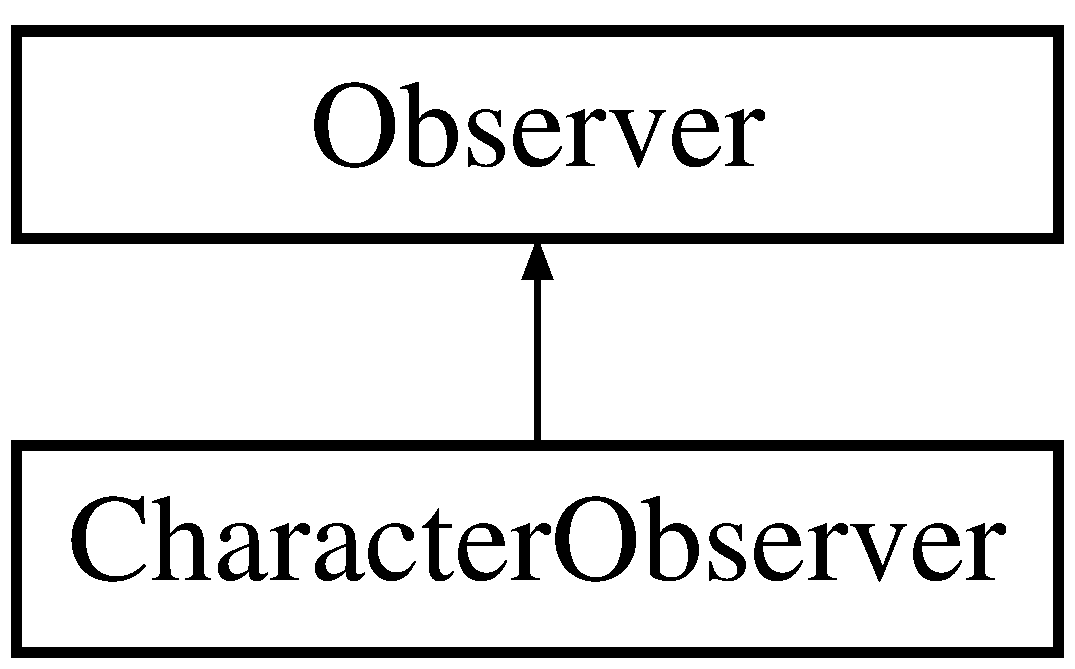
\includegraphics[height=2.000000cm]{class_character_observer}
\end{center}
\end{figure}
\subsection*{Public Member Functions}
\begin{DoxyCompactItemize}
\item 
\hypertarget{class_character_observer_a254ed3594bea4060cebb8f00dcf313b0}{}\label{class_character_observer_a254ed3594bea4060cebb8f00dcf313b0} 
\hyperlink{class_character_observer_a254ed3594bea4060cebb8f00dcf313b0}{Character\+Observer} ()
\begin{DoxyCompactList}\small\item\em \hyperlink{class_character_observer}{Character\+Observer} default constructor. \end{DoxyCompactList}\item 
\hyperlink{class_character_observer_a6a215cb4cdb72aabc0ad95b8b7c0373c}{Character\+Observer} (\hyperlink{class_character}{Character} $\ast$c)
\item 
\hypertarget{class_character_observer_ac535a0d01c7ab57f41b933a9507116fb}{}\label{class_character_observer_ac535a0d01c7ab57f41b933a9507116fb} 
\hyperlink{class_character_observer_ac535a0d01c7ab57f41b933a9507116fb}{$\sim$\+Character\+Observer} ()
\begin{DoxyCompactList}\small\item\em Destructor that detaches the \hyperlink{class_character_observer}{Character\+Observer} from the subject (\hyperlink{class_character}{Character}) \end{DoxyCompactList}\item 
\hypertarget{class_character_observer_a398d6d784065c7ed36c928d44a574630}{}\label{class_character_observer_a398d6d784065c7ed36c928d44a574630} 
void \hyperlink{class_character_observer_a398d6d784065c7ed36c928d44a574630}{Update} ()
\begin{DoxyCompactList}\small\item\em Function that is called by Notify() when the state of the underlying subject object changes. \end{DoxyCompactList}\item 
\hypertarget{class_character_observer_af255a3fd431b55de8dd2ab9a639e546b}{}\label{class_character_observer_af255a3fd431b55de8dd2ab9a639e546b} 
void \hyperlink{class_character_observer_af255a3fd431b55de8dd2ab9a639e546b}{display} ()
\begin{DoxyCompactList}\small\item\em Function that displays the character\textquotesingle{}s attributes to the console window to demonstrate changes to subject. \end{DoxyCompactList}\end{DoxyCompactItemize}
\subsection*{Additional Inherited Members}


\subsection{Detailed Description}
Class that inherits from \hyperlink{class_observer}{Observer} and that implements \hyperlink{class_character_observer}{Character\+Observer}. 

\subsection{Constructor \& Destructor Documentation}
\hypertarget{class_character_observer_a6a215cb4cdb72aabc0ad95b8b7c0373c}{}\label{class_character_observer_a6a215cb4cdb72aabc0ad95b8b7c0373c} 
\index{Character\+Observer@{Character\+Observer}!Character\+Observer@{Character\+Observer}}
\index{Character\+Observer@{Character\+Observer}!Character\+Observer@{Character\+Observer}}
\subsubsection{\texorpdfstring{Character\+Observer()}{CharacterObserver()}}
{\footnotesize\ttfamily Character\+Observer\+::\+Character\+Observer (\begin{DoxyParamCaption}\item[{\hyperlink{class_character}{Character} $\ast$}]{c }\end{DoxyParamCaption})}

\hyperlink{class_character}{Character} observer parameterized constructor Upon instantiation, the \hyperlink{class_character_observer}{Character\+Observer} instantiates itself to a character 
\begin{DoxyParams}{Parameters}
{\em c} & Pointer to an object of type \hyperlink{class_character}{Character} \\
\hline
\end{DoxyParams}


The documentation for this class was generated from the following files\+:\begin{DoxyCompactItemize}
\item 
\hyperlink{_character_observer_8h}{Character\+Observer.\+h}\item 
\hyperlink{_character_observer_8cpp}{Character\+Observer.\+cpp}\end{DoxyCompactItemize}

\hypertarget{class_concrete_builder_a}{}\section{Concrete\+BuilderA Class Reference}
\label{class_concrete_builder_a}\index{Concrete\+BuilderA@{Concrete\+BuilderA}}


Class for the implementation of a concrete builder class which adapts contents of a map to the player\textquotesingle{}s level.  




{\ttfamily \#include $<$Concrete\+Builder\+A.\+h$>$}

Inheritance diagram for Concrete\+BuilderA\+:\begin{figure}[H]
\begin{center}
\leavevmode
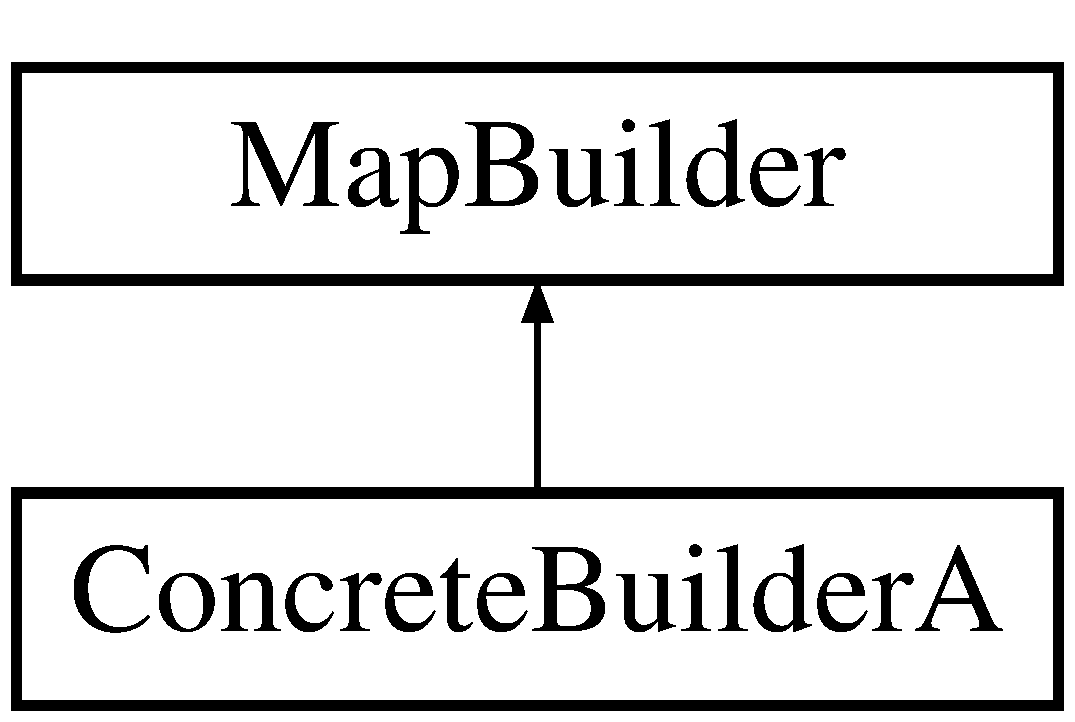
\includegraphics[height=2.000000cm]{class_concrete_builder_a}
\end{center}
\end{figure}
\subsection*{Public Member Functions}
\begin{DoxyCompactItemize}
\item 
void \hyperlink{class_concrete_builder_a_ae442fa67468d68f65814f730e674af2d}{build\+Character} (char, int, int, \hyperlink{class_map_object}{Map\+Object} $\ast$)
\begin{DoxyCompactList}\small\item\em non default constructor \end{DoxyCompactList}\item 
\hypertarget{class_concrete_builder_a_a153a45d8b1b6369c7c4bc2a360e0c2a5}{}\label{class_concrete_builder_a_a153a45d8b1b6369c7c4bc2a360e0c2a5} 
void \hyperlink{class_concrete_builder_a_a153a45d8b1b6369c7c4bc2a360e0c2a5}{build\+Container} (int, int, vector$<$ \hyperlink{class_item}{Item} $\ast$$>$ \&)
\begin{DoxyCompactList}\small\item\em Method to adapt a chest level to the player\textquotesingle{}s level. \end{DoxyCompactList}\end{DoxyCompactItemize}
\subsection*{Additional Inherited Members}


\subsection{Detailed Description}
Class for the implementation of a concrete builder class which adapts contents of a map to the player\textquotesingle{}s level. 

\subsection{Member Function Documentation}
\hypertarget{class_concrete_builder_a_ae442fa67468d68f65814f730e674af2d}{}\label{class_concrete_builder_a_ae442fa67468d68f65814f730e674af2d} 
\index{Concrete\+BuilderA@{Concrete\+BuilderA}!build\+Character@{build\+Character}}
\index{build\+Character@{build\+Character}!Concrete\+BuilderA@{Concrete\+BuilderA}}
\subsubsection{\texorpdfstring{build\+Character()}{buildCharacter()}}
{\footnotesize\ttfamily void Concrete\+Builder\+A\+::build\+Character (\begin{DoxyParamCaption}\item[{char}]{type,  }\item[{int}]{j,  }\item[{int}]{i,  }\item[{\hyperlink{class_map_object}{Map\+Object} $\ast$}]{character }\end{DoxyParamCaption})\hspace{0.3cm}{\ttfamily [virtual]}}



non default constructor 

Get all attributes of the enemy

Every time a character levels up, we assume the character gets two ability scores to be added any of to the current ability scores

Since the character is a fighter, a d10 hit dice was used to get a number that will be added or removed to the total and current hit points

After getting the ability scores bonus that must be assigned, randomly assign to one of the abilities. If the player level is higher than the current enemy level, it will increase some ability scores. If the player level is lower than the current enemy level, it will decrease some ability scores.

Max scores for an ability is 30, if it reaches 30, it won\textquotesingle{}t do anything

Calculate the difference between old and new constitution scores to figure out how many points must be added or removed from the hit points

Adjust the current and total hit points to the player\textquotesingle{}s level

Set all the attributes of the character 

Implements \hyperlink{class_map_builder}{Map\+Builder}.



The documentation for this class was generated from the following files\+:\begin{DoxyCompactItemize}
\item 
Concrete\+Builder\+A.\+h\item 
\hyperlink{_concrete_builder_a_8cpp}{Concrete\+Builder\+A.\+cpp}\end{DoxyCompactItemize}

\hypertarget{class_concrete_builder_b}{}\section{Concrete\+BuilderB Class Reference}
\label{class_concrete_builder_b}\index{Concrete\+BuilderB@{Concrete\+BuilderB}}


Class for the implementation of a concrete builder class which allows user editing of contents on map.  




{\ttfamily \#include $<$Concrete\+Builder\+B.\+h$>$}

Inheritance diagram for Concrete\+BuilderB\+:\begin{figure}[H]
\begin{center}
\leavevmode
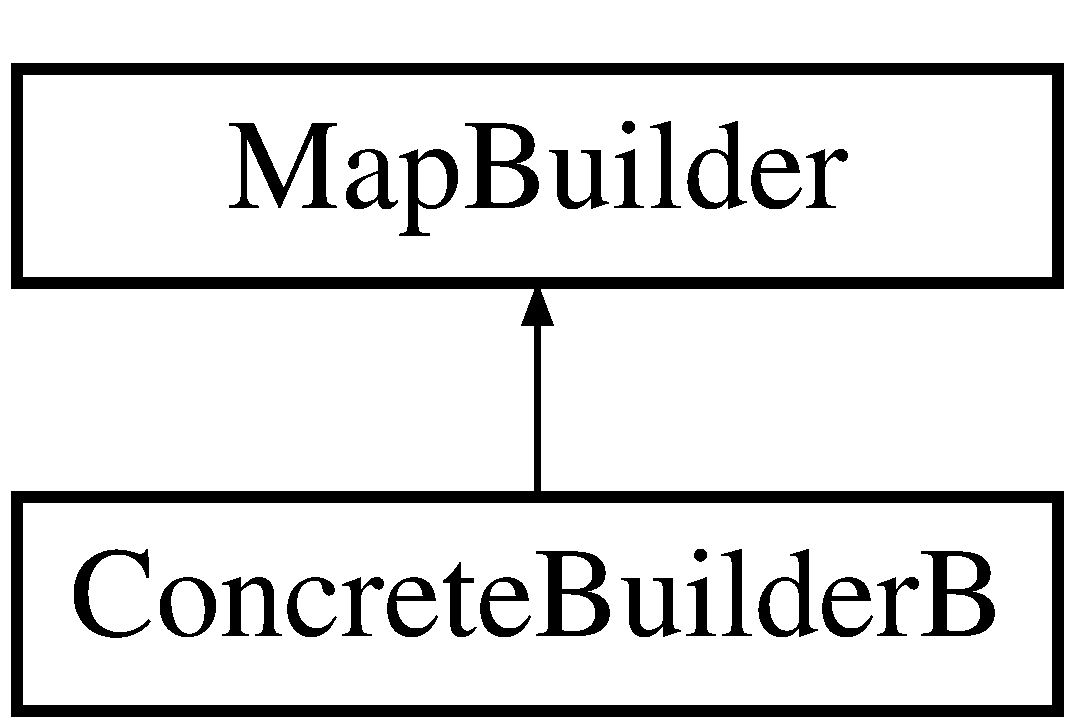
\includegraphics[height=2.000000cm]{class_concrete_builder_b}
\end{center}
\end{figure}
\subsection*{Public Member Functions}
\begin{DoxyCompactItemize}
\item 
\hypertarget{class_concrete_builder_b_a71b5a6a7cd48a512c3eae536d95c41cf}{}\label{class_concrete_builder_b_a71b5a6a7cd48a512c3eae536d95c41cf} 
void {\bfseries build\+Character} (char, int, int, \hyperlink{class_map_object}{Map\+Object} $\ast$)
\item 
\hypertarget{class_concrete_builder_b_a789bea926798f77e30fba68fab1f48bc}{}\label{class_concrete_builder_b_a789bea926798f77e30fba68fab1f48bc} 
void {\bfseries build\+Container} (int, int)
\end{DoxyCompactItemize}
\subsection*{Additional Inherited Members}


\subsection{Detailed Description}
Class for the implementation of a concrete builder class which allows user editing of contents on map. 

The documentation for this class was generated from the following files\+:\begin{DoxyCompactItemize}
\item 
Concrete\+Builder\+B.\+h\item 
\hyperlink{_concrete_builder_b_8cpp}{Concrete\+Builder\+B.\+cpp}\end{DoxyCompactItemize}

\hypertarget{class_console_view}{}\section{Console\+View Class Reference}
\label{class_console_view}\index{Console\+View@{Console\+View}}


Class that inherits from \hyperlink{class_observer}{Observer}.  




{\ttfamily \#include $<$Console\+View.\+h$>$}

Inheritance diagram for Console\+View\+:\begin{figure}[H]
\begin{center}
\leavevmode
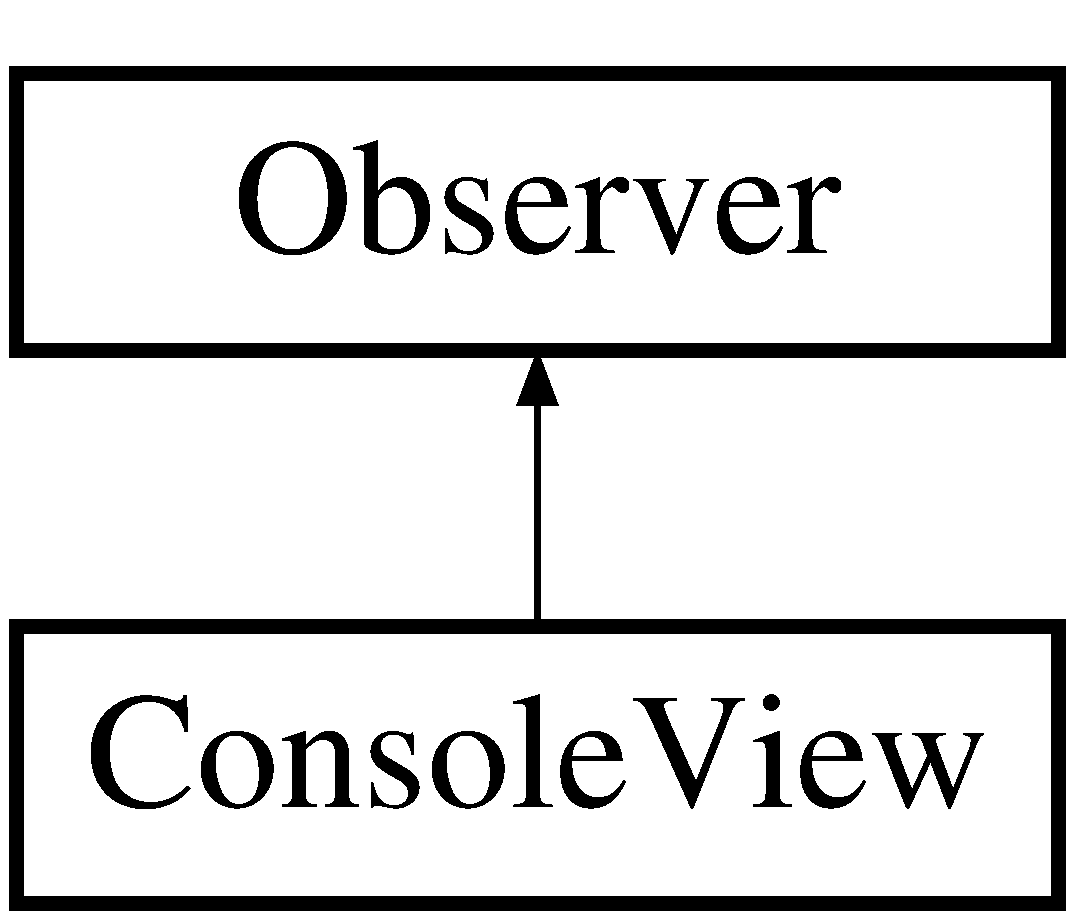
\includegraphics[height=2.000000cm]{class_console_view}
\end{center}
\end{figure}
\subsection*{Public Member Functions}
\begin{DoxyCompactItemize}
\item 
\hypertarget{class_console_view_afb9bf13f2b254d98756e8ac7b71836b5}{}\label{class_console_view_afb9bf13f2b254d98756e8ac7b71836b5} 
\hyperlink{class_console_view_afb9bf13f2b254d98756e8ac7b71836b5}{Console\+View} ()
\begin{DoxyCompactList}\small\item\em default constructor \end{DoxyCompactList}\item 
\hyperlink{class_console_view_a9f6167ddbbfea6f768de7ed5d8694f6e}{Console\+View} (\hyperlink{class_map_play}{Map\+Play} $\ast$s)
\item 
\hypertarget{class_console_view_a4efef4d1fbd8bece5d3a2f65964c3e1f}{}\label{class_console_view_a4efef4d1fbd8bece5d3a2f65964c3e1f} 
\hyperlink{class_console_view_a4efef4d1fbd8bece5d3a2f65964c3e1f}{$\sim$\+Console\+View} ()
\begin{DoxyCompactList}\small\item\em Upon destruction, detaches itself from \hyperlink{class_map_play}{Map\+Play}. \end{DoxyCompactList}\item 
\hypertarget{class_console_view_aa082d34551ba481dcaf536dd2532288e}{}\label{class_console_view_aa082d34551ba481dcaf536dd2532288e} 
void \hyperlink{class_console_view_aa082d34551ba481dcaf536dd2532288e}{Update} ()
\begin{DoxyCompactList}\small\item\em method to update the view as the changes are made by concrete subject, after being notified by the latter \end{DoxyCompactList}\item 
\hypertarget{class_console_view_a7dd53ef05cf17f16f2a09be3ed8f0fab}{}\label{class_console_view_a7dd53ef05cf17f16f2a09be3ed8f0fab} 
void \hyperlink{class_console_view_a7dd53ef05cf17f16f2a09be3ed8f0fab}{display} ()
\begin{DoxyCompactList}\small\item\em method to print double array on console \end{DoxyCompactList}\end{DoxyCompactItemize}
\subsection*{Additional Inherited Members}


\subsection{Detailed Description}
Class that inherits from \hyperlink{class_observer}{Observer}. 

\subsection{Constructor \& Destructor Documentation}
\hypertarget{class_console_view_a9f6167ddbbfea6f768de7ed5d8694f6e}{}\label{class_console_view_a9f6167ddbbfea6f768de7ed5d8694f6e} 
\index{Console\+View@{Console\+View}!Console\+View@{Console\+View}}
\index{Console\+View@{Console\+View}!Console\+View@{Console\+View}}
\subsubsection{\texorpdfstring{Console\+View()}{ConsoleView()}}
{\footnotesize\ttfamily Console\+View\+::\+Console\+View (\begin{DoxyParamCaption}\item[{\hyperlink{class_map_play}{Map\+Play} $\ast$}]{s }\end{DoxyParamCaption})}

Upon instantiation, attaches itself to a \hyperlink{class_map_play}{Map\+Play} 
\begin{DoxyParams}{Parameters}
{\em s} & = a \hyperlink{class_map_play}{Map\+Play} instance \\
\hline
\end{DoxyParams}


The documentation for this class was generated from the following files\+:\begin{DoxyCompactItemize}
\item 
\hyperlink{_console_view_8h}{Console\+View.\+h}\item 
\hyperlink{_console_view_8cpp}{Console\+View.\+cpp}\end{DoxyCompactItemize}

\hypertarget{class_dice}{}\section{Dice Class Reference}
\label{class_dice}\index{Dice@{Dice}}


class that implements the rolling of \hyperlink{class_dice}{Dice}  




{\ttfamily \#include $<$Dice.\+h$>$}

\subsection*{Static Public Member Functions}
\begin{DoxyCompactItemize}
\item 
static int \hyperlink{class_dice_a9d062543cd55b9ccad4649f80a970e10}{roll} (string dice\+String)
\item 
static bool \hyperlink{class_dice_add8db0b3ba7cd229a3b3cea3ee87fcad}{is\+Valid} (string test)
\end{DoxyCompactItemize}


\subsection{Detailed Description}
class that implements the rolling of \hyperlink{class_dice}{Dice} 

\subsection{Member Function Documentation}
\hypertarget{class_dice_add8db0b3ba7cd229a3b3cea3ee87fcad}{}\label{class_dice_add8db0b3ba7cd229a3b3cea3ee87fcad} 
\index{Dice@{Dice}!is\+Valid@{is\+Valid}}
\index{is\+Valid@{is\+Valid}!Dice@{Dice}}
\subsubsection{\texorpdfstring{is\+Valid()}{isValid()}}
{\footnotesize\ttfamily bool Dice\+::is\+Valid (\begin{DoxyParamCaption}\item[{string}]{test }\end{DoxyParamCaption})\hspace{0.3cm}{\ttfamily [static]}}

Checks if input string is syntatically valid 
\begin{DoxyParams}{Parameters}
{\em test} & \+: a string test that needs to be validated \\
\hline
\end{DoxyParams}
\begin{DoxyReturn}{Returns}
true or false 
\end{DoxyReturn}
\hypertarget{class_dice_a9d062543cd55b9ccad4649f80a970e10}{}\label{class_dice_a9d062543cd55b9ccad4649f80a970e10} 
\index{Dice@{Dice}!roll@{roll}}
\index{roll@{roll}!Dice@{Dice}}
\subsubsection{\texorpdfstring{roll()}{roll()}}
{\footnotesize\ttfamily int Dice\+::roll (\begin{DoxyParamCaption}\item[{string}]{dice\+String }\end{DoxyParamCaption})\hspace{0.3cm}{\ttfamily [static]}}

Main funtion to roll the dice 
\begin{DoxyParams}{Parameters}
{\em dice\+String} & \+: string input containing dice info \\
\hline
\end{DoxyParams}
\begin{DoxyReturn}{Returns}
result of the roll 
\end{DoxyReturn}


The documentation for this class was generated from the following files\+:\begin{DoxyCompactItemize}
\item 
\hyperlink{_dice_8h}{Dice.\+h}\item 
\hyperlink{_dice_8cpp}{Dice.\+cpp}\end{DoxyCompactItemize}

\hypertarget{class_editor_g_u_i}{}\section{Editor\+G\+UI Class Reference}
\label{class_editor_g_u_i}\index{Editor\+G\+UI@{Editor\+G\+UI}}
\subsection*{Public Member Functions}
\begin{DoxyCompactItemize}
\item 
\hyperlink{class_editor_g_u_i_a9b5d98aacd3392b5c8f15b0a7e305bed}{Editor\+G\+UI} (sf\+::\+Render\+Window \&window)
\item 
\hypertarget{class_editor_g_u_i_a3fa7a8b494f2d6db6a871b53e3c670ff}{}\label{class_editor_g_u_i_a3fa7a8b494f2d6db6a871b53e3c670ff} 
void \hyperlink{class_editor_g_u_i_a3fa7a8b494f2d6db6a871b53e3c670ff}{open\+Editor\+Window} ()
\begin{DoxyCompactList}\small\item\em Implementation of open\+Editor\+Window to allow selection of map editor or campaign editor. \end{DoxyCompactList}\item 
\hypertarget{class_editor_g_u_i_af427d199861fff95e333113aeb4b1dcb}{}\label{class_editor_g_u_i_af427d199861fff95e333113aeb4b1dcb} 
void \hyperlink{class_editor_g_u_i_af427d199861fff95e333113aeb4b1dcb}{open\+Map\+Editor\+Window} ()
\begin{DoxyCompactList}\small\item\em Implementation of open\+Map\+Editor\+Window to initialize map editor. \end{DoxyCompactList}\item 
\hypertarget{class_editor_g_u_i_a4857cb67f85c8f8a4213e5718d44316b}{}\label{class_editor_g_u_i_a4857cb67f85c8f8a4213e5718d44316b} 
void \hyperlink{class_editor_g_u_i_a4857cb67f85c8f8a4213e5718d44316b}{open\+New\+Map\+Window} ()
\begin{DoxyCompactList}\small\item\em Implementation of open\+New\+Map\+Window to select the size of the new map. \end{DoxyCompactList}\item 
\hypertarget{class_editor_g_u_i_ae36efa4acd276b709953c277601f5768}{}\label{class_editor_g_u_i_ae36efa4acd276b709953c277601f5768} 
void \hyperlink{class_editor_g_u_i_ae36efa4acd276b709953c277601f5768}{open\+Load\+Map\+Window} ()
\begin{DoxyCompactList}\small\item\em Implementation of open\+Load\+Map\+Window to select the map to load and edit. \end{DoxyCompactList}\item 
\hypertarget{class_editor_g_u_i_a83f04b7568d9e6df9fd9c11ac1ce5154}{}\label{class_editor_g_u_i_a83f04b7568d9e6df9fd9c11ac1ce5154} 
void \hyperlink{class_editor_g_u_i_a83f04b7568d9e6df9fd9c11ac1ce5154}{open\+Map\+View} ()
\begin{DoxyCompactList}\small\item\em Implementation of open\+Map\+View to see and edit a map. \end{DoxyCompactList}\item 
\hypertarget{class_editor_g_u_i_a8666109538677294c6c0ff887fabe3b4}{}\label{class_editor_g_u_i_a8666109538677294c6c0ff887fabe3b4} 
void \hyperlink{class_editor_g_u_i_a8666109538677294c6c0ff887fabe3b4}{open\+Campaign\+Editor\+Window} ()
\begin{DoxyCompactList}\small\item\em Impelmentation of open\+Campaign\+Editor\+Window to initalize campaign editor. \end{DoxyCompactList}\item 
\hypertarget{class_editor_g_u_i_ab01a34e8ee51e9ea4d875768963fd4fa}{}\label{class_editor_g_u_i_ab01a34e8ee51e9ea4d875768963fd4fa} 
void \hyperlink{class_editor_g_u_i_ab01a34e8ee51e9ea4d875768963fd4fa}{open\+Map\+List\+Selection\+Window} ()
\begin{DoxyCompactList}\small\item\em Implementation of open\+Map\+List\+Selection\+Window to select the maps to add to a campaign. \end{DoxyCompactList}\item 
\hypertarget{class_editor_g_u_i_a1ad2c0ab996ad413ac5230234d79e6ea}{}\label{class_editor_g_u_i_a1ad2c0ab996ad413ac5230234d79e6ea} 
void \hyperlink{class_editor_g_u_i_a1ad2c0ab996ad413ac5230234d79e6ea}{open\+Load\+Campaign\+Window} ()
\begin{DoxyCompactList}\small\item\em Implementation of open\+Load\+Campaign\+Window to display and select the available campaigns to load. \end{DoxyCompactList}\item 
\hypertarget{class_editor_g_u_i_a63091d9097bf68884ff86f3d8be44cf6}{}\label{class_editor_g_u_i_a63091d9097bf68884ff86f3d8be44cf6} 
void \hyperlink{class_editor_g_u_i_a63091d9097bf68884ff86f3d8be44cf6}{open\+Campaign\+View} ()
\begin{DoxyCompactList}\small\item\em Implementation of open\+Campaign\+View to preview the campaign maps. \end{DoxyCompactList}\item 
\hypertarget{class_editor_g_u_i_a1a7889ca377931974866645202059ed4}{}\label{class_editor_g_u_i_a1a7889ca377931974866645202059ed4} 
void \hyperlink{class_editor_g_u_i_a1a7889ca377931974866645202059ed4}{Start} ()
\begin{DoxyCompactList}\small\item\em Implementation of Start to initialize the editor to the first state and the first view. \end{DoxyCompactList}\item 
\hypertarget{class_editor_g_u_i_a23bbbfa7a03460a82f94204636928ea5}{}\label{class_editor_g_u_i_a23bbbfa7a03460a82f94204636928ea5} 
void \hyperlink{class_editor_g_u_i_a23bbbfa7a03460a82f94204636928ea5}{Update} ()
\begin{DoxyCompactList}\small\item\em Implementation of Update to change the state of the editor. \end{DoxyCompactList}\item 
\hypertarget{class_editor_g_u_i_ac24768dd57d990712ac59f77d6c65d65}{}\label{class_editor_g_u_i_ac24768dd57d990712ac59f77d6c65d65} 
void \hyperlink{class_editor_g_u_i_ac24768dd57d990712ac59f77d6c65d65}{Display} ()
\begin{DoxyCompactList}\small\item\em Implementation of Display to change the view according to the current state. \end{DoxyCompactList}\item 
\hypertarget{class_editor_g_u_i_a75a38ddb623e90b00d69eeacf04c71ce}{}\label{class_editor_g_u_i_a75a38ddb623e90b00d69eeacf04c71ce} 
\hyperlink{class_editor_g_u_i_a75a38ddb623e90b00d69eeacf04c71ce}{$\sim$\+Editor\+G\+UI} ()
\begin{DoxyCompactList}\small\item\em Implementation of default destructor. \end{DoxyCompactList}\end{DoxyCompactItemize}
\subsection*{Static Public Attributes}
\begin{DoxyCompactItemize}
\item 
\hypertarget{class_editor_g_u_i_a47758bdf3d67da6c4516bc5d6fd1bdec}{}\label{class_editor_g_u_i_a47758bdf3d67da6c4516bc5d6fd1bdec} 
static const int {\bfseries W\+I\+N\+D\+O\+W\+\_\+\+S\+C\+A\+LE} = 800
\end{DoxyCompactItemize}


\subsection{Constructor \& Destructor Documentation}
\hypertarget{class_editor_g_u_i_a9b5d98aacd3392b5c8f15b0a7e305bed}{}\label{class_editor_g_u_i_a9b5d98aacd3392b5c8f15b0a7e305bed} 
\index{Editor\+G\+UI@{Editor\+G\+UI}!Editor\+G\+UI@{Editor\+G\+UI}}
\index{Editor\+G\+UI@{Editor\+G\+UI}!Editor\+G\+UI@{Editor\+G\+UI}}
\subsubsection{\texorpdfstring{Editor\+G\+U\+I()}{EditorGUI()}}
{\footnotesize\ttfamily Editor\+G\+U\+I\+::\+Editor\+G\+UI (\begin{DoxyParamCaption}\item[{sf\+::\+Render\+Window \&}]{new\+Window }\end{DoxyParamCaption})}

Implementation of non default constructor for \hyperlink{class_editor_g_u_i}{Editor\+G\+UI} class 
\begin{DoxyParams}{Parameters}
{\em new\+Window} & \+: a reference to a Render\+Window value \\
\hline
{\em new\+Map\+Editor} & \+: pointer to a new\+Map\+Editor object \\
\hline
{\em new\+Campaign\+Editor} & \+: pointer \\
\hline
\end{DoxyParams}


The documentation for this class was generated from the following files\+:\begin{DoxyCompactItemize}
\item 
\hyperlink{_editor_g_u_i_8h}{Editor\+G\+U\+I.\+h}\item 
\hyperlink{_editor_g_u_i_8cpp}{Editor\+G\+U\+I.\+cpp}\end{DoxyCompactItemize}

\hypertarget{class_enhancement}{}\section{Enhancement Class Reference}
\label{class_enhancement}\index{Enhancement@{Enhancement}}


Class for the implementation of an enhancement, i.\+e. a stat influenced by an item, as well as the bonus it gives.  




{\ttfamily \#include $<$Enhancement.\+h$>$}

\subsection*{Public Member Functions}
\begin{DoxyCompactItemize}
\item 
\hypertarget{class_enhancement_ab348c08841ab57c76daa7c3eab2ad4a3}{}\label{class_enhancement_ab348c08841ab57c76daa7c3eab2ad4a3} 
\hyperlink{class_enhancement_ab348c08841ab57c76daa7c3eab2ad4a3}{Enhancement} ()
\begin{DoxyCompactList}\small\item\em Default constructor. \end{DoxyCompactList}\item 
\hypertarget{class_enhancement_a202f69a38ce77d83f2dc536b793cc5bf}{}\label{class_enhancement_a202f69a38ce77d83f2dc536b793cc5bf} 
$<$$<$$<$$<$$<$$<$$<$ H\+E\+AD \hyperlink{class_enhancement}{Enhancement}(string type, int bonus);=======\hyperlink{class_enhancement}{Enhancement}(string, int);$>$$>$$>$$>$$>$$>$ string {\bfseries get\+Type} ()
\item 
\hypertarget{class_enhancement_afd0ea7d414468cf507a4673fd066fd89}{}\label{class_enhancement_afd0ea7d414468cf507a4673fd066fd89} 
int \hyperlink{class_enhancement_afd0ea7d414468cf507a4673fd066fd89}{get\+Bonus} ()
\begin{DoxyCompactList}\small\item\em Method to get the bonus of the enhancement. \end{DoxyCompactList}\item 
\hypertarget{class_enhancement_a01af1fd499599912e18fa11124f8dff9}{}\label{class_enhancement_a01af1fd499599912e18fa11124f8dff9} 
void {\bfseries set\+Bonus} (int)
\end{DoxyCompactItemize}
\subsection*{Friends}
\begin{DoxyCompactItemize}
\item 
\hypertarget{class_enhancement_ac98d07dd8f7b70e16ccb9a01abf56b9c}{}\label{class_enhancement_ac98d07dd8f7b70e16ccb9a01abf56b9c} 
class {\bfseries boost\+::serialization\+::access}
\end{DoxyCompactItemize}


\subsection{Detailed Description}
Class for the implementation of an enhancement, i.\+e. a stat influenced by an item, as well as the bonus it gives. 

The documentation for this class was generated from the following file\+:\begin{DoxyCompactItemize}
\item 
\hyperlink{_enhancement_8h}{Enhancement.\+h}\end{DoxyCompactItemize}

\hypertarget{class_game_state}{}\section{Game\+State Class Reference}
\label{class_game_state}\index{Game\+State@{Game\+State}}
\subsection*{Public Member Functions}
\begin{DoxyCompactItemize}
\item 
\hypertarget{class_game_state_a52aa15b9c112bf6bddbd1aac28d4ad88}{}\label{class_game_state_a52aa15b9c112bf6bddbd1aac28d4ad88} 
void {\bfseries set\+Map\+Editor\+State} (Map\+Editor\+State state)
\item 
\hypertarget{class_game_state_a9cb332e60c0e86369b424eb7cc7239ed}{}\label{class_game_state_a9cb332e60c0e86369b424eb7cc7239ed} 
void {\bfseries set\+Campaign\+Editor\+State} (Campaign\+Editor\+State state)
\item 
\hypertarget{class_game_state_a9534000297c35f215fb1d08112721e5c}{}\label{class_game_state_a9534000297c35f215fb1d08112721e5c} 
void {\bfseries set\+Editor\+State} (Editor\+State state)
\item 
\hypertarget{class_game_state_a97138a9485c9efd6159f6c19e055fa5a}{}\label{class_game_state_a97138a9485c9efd6159f6c19e055fa5a} 
void {\bfseries set\+Launch\+State} (Launch\+State state)
\item 
\hypertarget{class_game_state_aa771fc394545431feba185d6ef2fd650}{}\label{class_game_state_aa771fc394545431feba185d6ef2fd650} 
void {\bfseries set\+Active} (bool active)
\item 
\hypertarget{class_game_state_a50330237ac360a3afe5622ddce7449e1}{}\label{class_game_state_a50330237ac360a3afe5622ddce7449e1} 
void {\bfseries set\+Play\+State} (Play\+State state)
\item 
\hypertarget{class_game_state_adca8384a3cf8a6d77796d0244c53cb80}{}\label{class_game_state_adca8384a3cf8a6d77796d0244c53cb80} 
Map\+Editor\+State {\bfseries get\+Map\+Editor\+State} ()
\item 
\hypertarget{class_game_state_a25fb638bf3803b4e3eeb1244f47b69d3}{}\label{class_game_state_a25fb638bf3803b4e3eeb1244f47b69d3} 
Campaign\+Editor\+State {\bfseries get\+Campaign\+Editor\+State} ()
\item 
\hypertarget{class_game_state_a42a7b1a44d269c1abf60da64f5e2a550}{}\label{class_game_state_a42a7b1a44d269c1abf60da64f5e2a550} 
Editor\+State {\bfseries get\+Editor\+State} ()
\item 
\hypertarget{class_game_state_a7e693ac7e9a1c3898f2fd5a8db982773}{}\label{class_game_state_a7e693ac7e9a1c3898f2fd5a8db982773} 
Launch\+State {\bfseries get\+Launch\+State} ()
\item 
\hypertarget{class_game_state_aaa126995c9032521853d155b7df3e466}{}\label{class_game_state_aaa126995c9032521853d155b7df3e466} 
Play\+State {\bfseries get\+Play\+State} ()
\item 
\hypertarget{class_game_state_a1adfc2d4f8a3f2fd4d191309b4f5e6f3}{}\label{class_game_state_a1adfc2d4f8a3f2fd4d191309b4f5e6f3} 
bool {\bfseries is\+Active} ()
\end{DoxyCompactItemize}
\subsection*{Static Public Attributes}
\begin{DoxyCompactItemize}
\item 
\hypertarget{class_game_state_acb273d0f4a997287f1514c869195b587}{}\label{class_game_state_acb273d0f4a997287f1514c869195b587} 
static const int {\bfseries W\+I\+N\+D\+O\+W\+\_\+\+S\+C\+A\+LE} = 800
\end{DoxyCompactItemize}


The documentation for this class was generated from the following files\+:\begin{DoxyCompactItemize}
\item 
\hyperlink{_game_state_8h}{Game\+State.\+h}\item 
\hyperlink{_game_state_8cpp}{Game\+State.\+cpp}\end{DoxyCompactItemize}

\hypertarget{class_helmet}{}\section{Helmet Class Reference}
\label{class_helmet}\index{Helmet@{Helmet}}


Class for the implementation of a helmet.  




{\ttfamily \#include $<$Helmet.\+h$>$}

Inheritance diagram for Helmet\+:\begin{figure}[H]
\begin{center}
\leavevmode
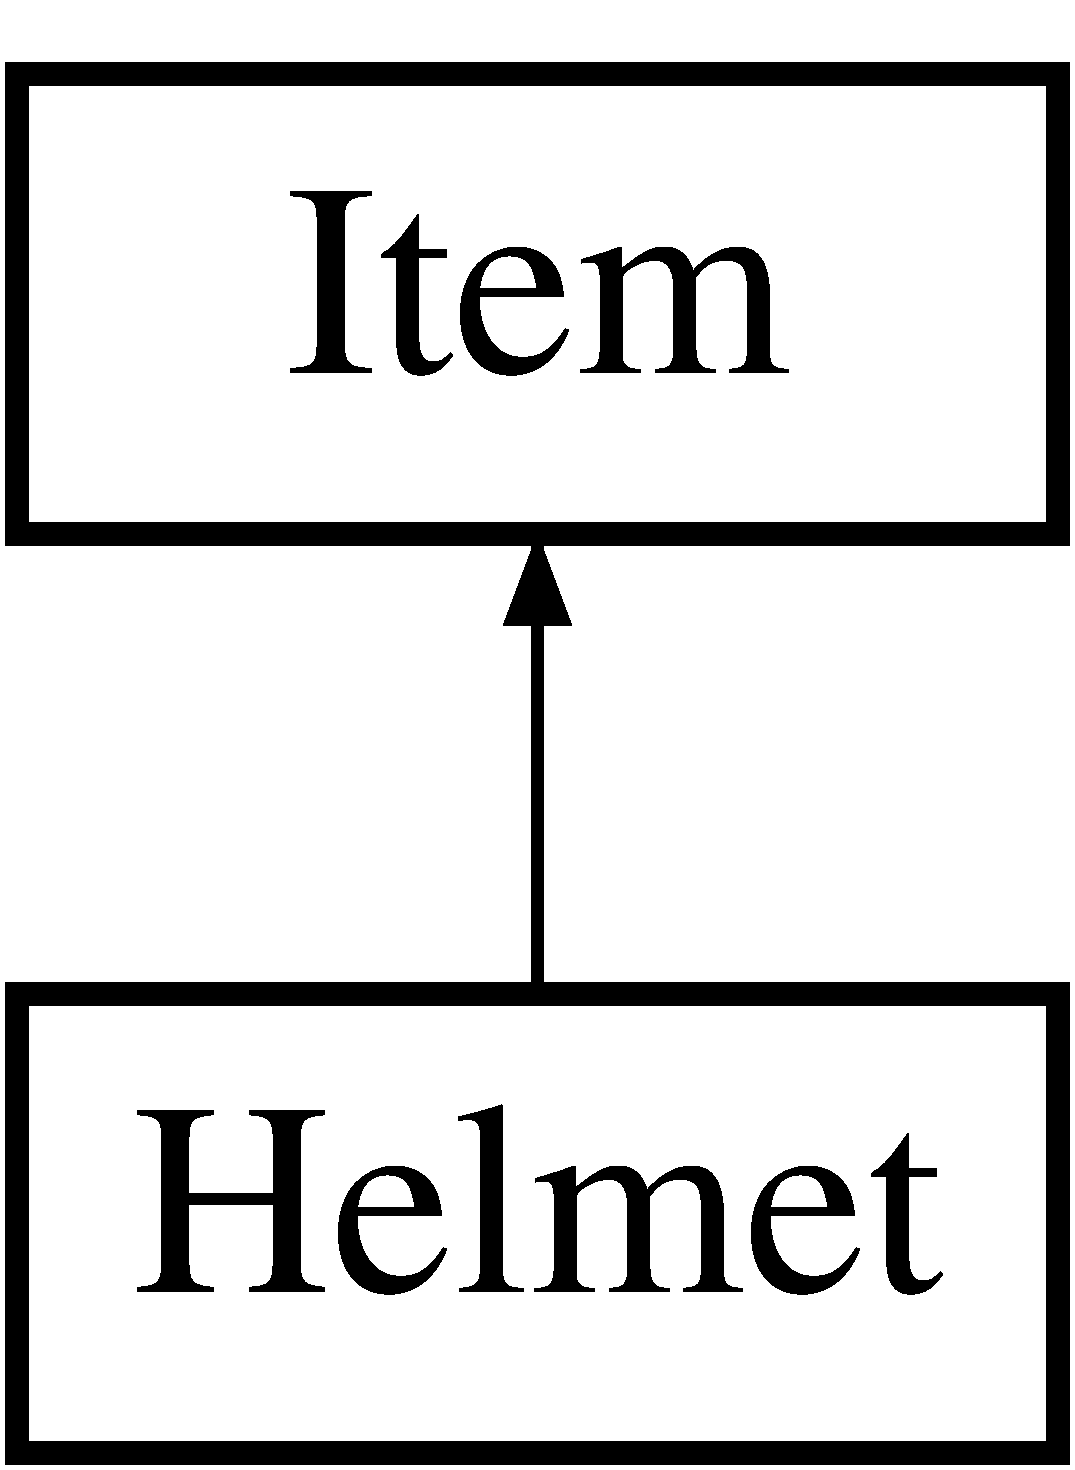
\includegraphics[height=2.000000cm]{class_helmet}
\end{center}
\end{figure}
\subsection*{Public Member Functions}
\begin{DoxyCompactItemize}
\item 
\hypertarget{class_helmet_ae9f39c8ca82962c770f9907123e663f5}{}\label{class_helmet_ae9f39c8ca82962c770f9907123e663f5} 
\hyperlink{class_helmet_ae9f39c8ca82962c770f9907123e663f5}{Helmet} ()
\begin{DoxyCompactList}\small\item\em Default constructor. \end{DoxyCompactList}\item 
\hyperlink{class_helmet_a527f044873f7a81dfcd6df549ba6e25d}{Helmet} (string name, int intelligence, int wisdom, int armor\+Class)
\item 
\hyperlink{class_helmet_a9d7a5c9a98e83c6a24545261aabcf120}{Helmet} (string name, vector$<$ \hyperlink{class_enhancement}{Enhancement} $>$ enhancements)
\item 
bool \hyperlink{class_helmet_aa840a7be0b69b5b3d60398c22d00537f}{validate\+Item} ()
\end{DoxyCompactItemize}
\subsection*{Friends}
\begin{DoxyCompactItemize}
\item 
\hypertarget{class_helmet_ac98d07dd8f7b70e16ccb9a01abf56b9c}{}\label{class_helmet_ac98d07dd8f7b70e16ccb9a01abf56b9c} 
class \hyperlink{class_helmet_ac98d07dd8f7b70e16ccb9a01abf56b9c}{boost\+::serialization\+::access}
\begin{DoxyCompactList}\small\item\em serialization \end{DoxyCompactList}\end{DoxyCompactItemize}
\subsection*{Additional Inherited Members}


\subsection{Detailed Description}
Class for the implementation of a helmet. 

\subsection{Constructor \& Destructor Documentation}
\hypertarget{class_helmet_a527f044873f7a81dfcd6df549ba6e25d}{}\label{class_helmet_a527f044873f7a81dfcd6df549ba6e25d} 
\index{Helmet@{Helmet}!Helmet@{Helmet}}
\index{Helmet@{Helmet}!Helmet@{Helmet}}
\subsubsection{\texorpdfstring{Helmet()}{Helmet()}\hspace{0.1cm}{\footnotesize\ttfamily [1/2]}}
{\footnotesize\ttfamily Helmet\+::\+Helmet (\begin{DoxyParamCaption}\item[{string}]{name,  }\item[{int}]{intelligence\+Bonus,  }\item[{int}]{wisdom\+Bonus,  }\item[{int}]{armor\+Class\+Bonus }\end{DoxyParamCaption})}

Constructor that calls an \hyperlink{class_item}{Item} constructor 
\begin{DoxyParams}{Parameters}
{\em intelligence\+Bonus} & \+: Integer representing the enhancement bonus for the stats Intelligence \\
\hline
{\em wisdom\+Bonus} & \+: Integer representing the enhancement bonus for the stats Wisdom \\
\hline
{\em armor\+Class\+Bonus} & \+: Integer representing the enhancement bonus for the stats \hyperlink{class_armor}{Armor} Class \\
\hline
\end{DoxyParams}
\hypertarget{class_helmet_a9d7a5c9a98e83c6a24545261aabcf120}{}\label{class_helmet_a9d7a5c9a98e83c6a24545261aabcf120} 
\index{Helmet@{Helmet}!Helmet@{Helmet}}
\index{Helmet@{Helmet}!Helmet@{Helmet}}
\subsubsection{\texorpdfstring{Helmet()}{Helmet()}\hspace{0.1cm}{\footnotesize\ttfamily [2/2]}}
{\footnotesize\ttfamily Helmet\+::\+Helmet (\begin{DoxyParamCaption}\item[{string}]{name,  }\item[{vector$<$ \hyperlink{class_enhancement}{Enhancement} $>$}]{enhancements }\end{DoxyParamCaption})}

Constructor taking a vector of enhancements as parameter It also calls an \hyperlink{class_item}{Item} constructor and pass a vector of enhancements as parameter. 
\begin{DoxyParams}{Parameters}
{\em enhancements} & \+: Vector of enhancements \\
\hline
\end{DoxyParams}


\subsection{Member Function Documentation}
\hypertarget{class_helmet_aa840a7be0b69b5b3d60398c22d00537f}{}\label{class_helmet_aa840a7be0b69b5b3d60398c22d00537f} 
\index{Helmet@{Helmet}!validate\+Item@{validate\+Item}}
\index{validate\+Item@{validate\+Item}!Helmet@{Helmet}}
\subsubsection{\texorpdfstring{validate\+Item()}{validateItem()}}
{\footnotesize\ttfamily bool Helmet\+::validate\+Item (\begin{DoxyParamCaption}{ }\end{DoxyParamCaption})\hspace{0.3cm}{\ttfamily [virtual]}}

Overrided method to validate that the armor only enhances \textquotesingle{}A\+R\+M\+OR C\+L\+A\+SS\textquotesingle{}, \textquotesingle{}W\+I\+S\+D\+OM\textquotesingle{} and \textquotesingle{}I\+N\+T\+E\+L\+L\+I\+G\+E\+N\+CE\textquotesingle{} and verify that the bonus values are within \mbox{[}1..5\mbox{]} \begin{DoxyReturn}{Returns}
True if the enhancement list is valid according to the rules, false if not 
\end{DoxyReturn}


Reimplemented from \hyperlink{class_item_a6603371b60aaded48f697975c81fc25b}{Item}.



The documentation for this class was generated from the following files\+:\begin{DoxyCompactItemize}
\item 
\hyperlink{_helmet_8h}{Helmet.\+h}\item 
\hyperlink{_helmet_8cpp}{Helmet.\+cpp}\end{DoxyCompactItemize}

\hypertarget{class_item}{}\section{Item Class Reference}
\label{class_item}\index{Item@{Item}}


Class for the implementation of items wearable by a character.  




{\ttfamily \#include $<$Item.\+h$>$}

Inheritance diagram for Item\+:\begin{figure}[H]
\begin{center}
\leavevmode
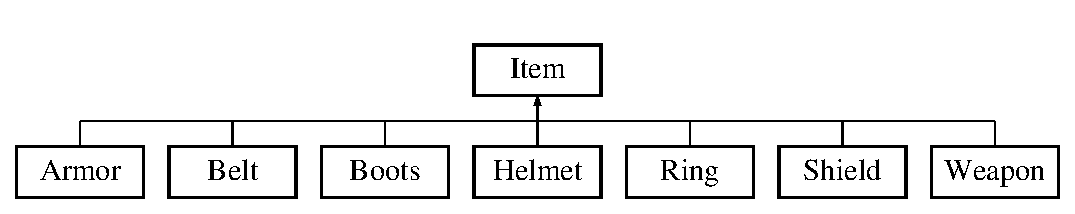
\includegraphics[height=2.000000cm]{class_item}
\end{center}
\end{figure}
\subsection*{Public Member Functions}
\begin{DoxyCompactItemize}
\item 
\hypertarget{class_item_a297720c02984eab37332ae795d22189d}{}\label{class_item_a297720c02984eab37332ae795d22189d} 
\hyperlink{class_item_a297720c02984eab37332ae795d22189d}{Item} ()
\begin{DoxyCompactList}\small\item\em Default constructor. \end{DoxyCompactList}\item 
\hyperlink{class_item_aa758d9160941f18ca7be38bc3835d5b9}{Item} (string type, string name, vector$<$ \hyperlink{class_enhancement}{Enhancement} $>$ enhancements)
\item 
string \hyperlink{class_item_a2aea1cc560205b01eaf5250c21f4fc71}{get\+Type} ()
\item 
string \hyperlink{class_item_a63d7f2148b699e539aae354b01559811}{get\+Name} ()
\item 
vector$<$ \hyperlink{class_enhancement}{Enhancement} $>$ \hyperlink{class_item_abf06eb8a8f73633c4c7c922073a754b8}{get\+Enhancements} ()
\item 
void \hyperlink{class_item_a5827bb049b61a0a95e448607d1247914}{add\+Enhancement} (\hyperlink{class_enhancement}{Enhancement} e)
\item 
void \hyperlink{class_item_a31da3e0fed93e6bcf2402e2c65259c2e}{set\+Enhancement\+Bonus} (int, int)
\item 
\hypertarget{class_item_a7be8022e6fe1a00d0fae058161d94977}{}\label{class_item_a7be8022e6fe1a00d0fae058161d94977} 
void \hyperlink{class_item_a7be8022e6fe1a00d0fae058161d94977}{display\+Enhancements} ()
\begin{DoxyCompactList}\small\item\em Method to display all the enhancements in the vector along with their respective bonus values. \end{DoxyCompactList}\item 
virtual bool \hyperlink{class_item_a6603371b60aaded48f697975c81fc25b}{validate\+Item} ()
\end{DoxyCompactItemize}
\subsection*{Protected Attributes}
\begin{DoxyCompactItemize}
\item 
\hypertarget{class_item_a5fddc3cf5f552ab8f5cceacaba430474}{}\label{class_item_a5fddc3cf5f552ab8f5cceacaba430474} 
string {\bfseries type}
\item 
\hypertarget{class_item_a406cde7962a6b42a66b4a53c9a26db2c}{}\label{class_item_a406cde7962a6b42a66b4a53c9a26db2c} 
string {\bfseries name}
\item 
\hypertarget{class_item_a0bc10f489737df2323ef72b2b225d504}{}\label{class_item_a0bc10f489737df2323ef72b2b225d504} 
vector$<$ \hyperlink{class_enhancement}{Enhancement} $>$ {\bfseries enhancements}
\end{DoxyCompactItemize}
\subsection*{Friends}
\begin{DoxyCompactItemize}
\item 
class \hyperlink{class_item_ac98d07dd8f7b70e16ccb9a01abf56b9c}{boost\+::serialization\+::access}
\end{DoxyCompactItemize}


\subsection{Detailed Description}
Class for the implementation of items wearable by a character. 

\subsection{Constructor \& Destructor Documentation}
\hypertarget{class_item_aa758d9160941f18ca7be38bc3835d5b9}{}\label{class_item_aa758d9160941f18ca7be38bc3835d5b9} 
\index{Item@{Item}!Item@{Item}}
\index{Item@{Item}!Item@{Item}}
\subsubsection{\texorpdfstring{Item()}{Item()}}
{\footnotesize\ttfamily Item\+::\+Item (\begin{DoxyParamCaption}\item[{string}]{type,  }\item[{string}]{name,  }\item[{vector$<$ \hyperlink{class_enhancement}{Enhancement} $>$}]{enhancements }\end{DoxyParamCaption})}

Constructor that receives an item type as a string and a vector containing the enhancements 
\begin{DoxyParams}{Parameters}
{\em type} & \+: String representing the type of item \\
\hline
{\em enhancements} & \+: Vector containing all the enhancements \\
\hline
\end{DoxyParams}


\subsection{Member Function Documentation}
\hypertarget{class_item_a5827bb049b61a0a95e448607d1247914}{}\label{class_item_a5827bb049b61a0a95e448607d1247914} 
\index{Item@{Item}!add\+Enhancement@{add\+Enhancement}}
\index{add\+Enhancement@{add\+Enhancement}!Item@{Item}}
\subsubsection{\texorpdfstring{add\+Enhancement()}{addEnhancement()}}
{\footnotesize\ttfamily void Item\+::add\+Enhancement (\begin{DoxyParamCaption}\item[{\hyperlink{class_enhancement}{Enhancement}}]{e }\end{DoxyParamCaption})}

Method to add an enhancement to the vector enhancements 
\begin{DoxyParams}{Parameters}
{\em e} & \+: \hyperlink{class_enhancement}{Enhancement} object \\
\hline
\end{DoxyParams}
\hypertarget{class_item_abf06eb8a8f73633c4c7c922073a754b8}{}\label{class_item_abf06eb8a8f73633c4c7c922073a754b8} 
\index{Item@{Item}!get\+Enhancements@{get\+Enhancements}}
\index{get\+Enhancements@{get\+Enhancements}!Item@{Item}}
\subsubsection{\texorpdfstring{get\+Enhancements()}{getEnhancements()}}
{\footnotesize\ttfamily vector$<$ \hyperlink{class_enhancement}{Enhancement} $>$ Item\+::get\+Enhancements (\begin{DoxyParamCaption}{ }\end{DoxyParamCaption})}

Method to get the enhancements of the item \begin{DoxyReturn}{Returns}
Vector containing a list of stats that the item enhances 
\end{DoxyReturn}
\hypertarget{class_item_a63d7f2148b699e539aae354b01559811}{}\label{class_item_a63d7f2148b699e539aae354b01559811} 
\index{Item@{Item}!get\+Name@{get\+Name}}
\index{get\+Name@{get\+Name}!Item@{Item}}
\subsubsection{\texorpdfstring{get\+Name()}{getName()}}
{\footnotesize\ttfamily string Item\+::get\+Name (\begin{DoxyParamCaption}{ }\end{DoxyParamCaption})}

Method to get the name of the item \begin{DoxyReturn}{Returns}
Name of the item 
\end{DoxyReturn}
\hypertarget{class_item_a2aea1cc560205b01eaf5250c21f4fc71}{}\label{class_item_a2aea1cc560205b01eaf5250c21f4fc71} 
\index{Item@{Item}!get\+Type@{get\+Type}}
\index{get\+Type@{get\+Type}!Item@{Item}}
\subsubsection{\texorpdfstring{get\+Type()}{getType()}}
{\footnotesize\ttfamily string Item\+::get\+Type (\begin{DoxyParamCaption}{ }\end{DoxyParamCaption})}

Method to get the type of the item \begin{DoxyReturn}{Returns}
Type of the item 
\end{DoxyReturn}
\hypertarget{class_item_a31da3e0fed93e6bcf2402e2c65259c2e}{}\label{class_item_a31da3e0fed93e6bcf2402e2c65259c2e} 
\index{Item@{Item}!set\+Enhancement\+Bonus@{set\+Enhancement\+Bonus}}
\index{set\+Enhancement\+Bonus@{set\+Enhancement\+Bonus}!Item@{Item}}
\subsubsection{\texorpdfstring{set\+Enhancement\+Bonus()}{setEnhancementBonus()}}
{\footnotesize\ttfamily void Item\+::set\+Enhancement\+Bonus (\begin{DoxyParamCaption}\item[{int}]{index,  }\item[{int}]{bonus }\end{DoxyParamCaption})}

Method to set the enhancement bonus of an enhancement 
\begin{DoxyParams}{Parameters}
{\em index} & \+: Index of the enhancement inside the vector \\
\hline
\end{DoxyParams}
\hypertarget{class_item_a6603371b60aaded48f697975c81fc25b}{}\label{class_item_a6603371b60aaded48f697975c81fc25b} 
\index{Item@{Item}!validate\+Item@{validate\+Item}}
\index{validate\+Item@{validate\+Item}!Item@{Item}}
\subsubsection{\texorpdfstring{validate\+Item()}{validateItem()}}
{\footnotesize\ttfamily bool Item\+::validate\+Item (\begin{DoxyParamCaption}{ }\end{DoxyParamCaption})\hspace{0.3cm}{\ttfamily [virtual]}}

Method to validate an item, e.\+g. verify that an item of a certain type only enhances a character statistic valid for this item type This method is overridden in the implementation of the subclasses for checking against the specific types of valid enhancement types. In the base class, it will only check that the bonus values are within \mbox{[}1..5\mbox{]}. \begin{DoxyReturn}{Returns}
True if the enhancement list is valid according to the rules, false if not 
\end{DoxyReturn}


Reimplemented in \hyperlink{class_ring_a9170e11e83f0a5b8443e9267e5bd6c8a}{Ring}, \hyperlink{class_belt_ab374477dd9d966e6e6b81b3699afd939}{Belt}, \hyperlink{class_boots_aac6123a5f117993f276eb5f2f343eeb0}{Boots}, \hyperlink{class_helmet_aa840a7be0b69b5b3d60398c22d00537f}{Helmet}, \hyperlink{class_shield_af28f146ed96720bd007a62a5871cd206}{Shield}, \hyperlink{class_weapon_afa7ce016c3cba686399cbe57628f8c70}{Weapon}, and \hyperlink{class_armor_a97b69f2691b172bd79e256a487a7f204}{Armor}.



\subsection{Friends And Related Function Documentation}
\hypertarget{class_item_ac98d07dd8f7b70e16ccb9a01abf56b9c}{}\label{class_item_ac98d07dd8f7b70e16ccb9a01abf56b9c} 
\index{Item@{Item}!boost\+::serialization\+::access@{boost\+::serialization\+::access}}
\index{boost\+::serialization\+::access@{boost\+::serialization\+::access}!Item@{Item}}
\subsubsection{\texorpdfstring{boost\+::serialization\+::access}{boost::serialization::access}}
{\footnotesize\ttfamily friend class boost\+::serialization\+::access\hspace{0.3cm}{\ttfamily [friend]}}

Serialization When the class Archive corresponds to an output archive, the \& operator is defined similar to $<$$<$. Likewise, when the class Archive is a type of input archive the \& operator is defined similar to $>$$>$. 

The documentation for this class was generated from the following files\+:\begin{DoxyCompactItemize}
\item 
\hyperlink{_item_8h}{Item.\+h}\item 
\hyperlink{_item_8cpp}{Item.\+cpp}\end{DoxyCompactItemize}

\hypertarget{class_item_container}{}\section{Item\+Container Class Reference}
\label{class_item_container}\index{Item\+Container@{Item\+Container}}


Class that implements an item container.  




{\ttfamily \#include $<$Item\+Container.\+h$>$}

Inheritance diagram for Item\+Container\+:\begin{figure}[H]
\begin{center}
\leavevmode
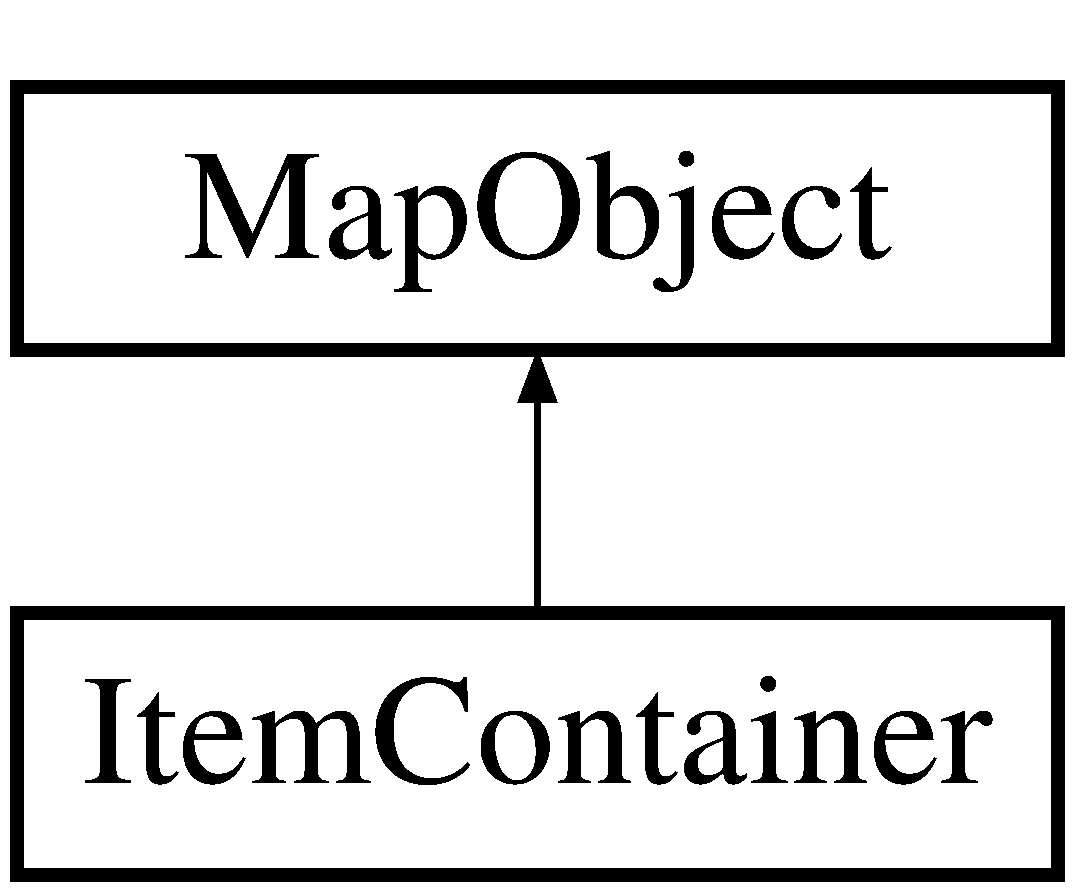
\includegraphics[height=2.000000cm]{class_item_container}
\end{center}
\end{figure}
\subsection*{Public Member Functions}
\begin{DoxyCompactItemize}
\item 
\hypertarget{class_item_container_a3ce79c8b4501fafc5ea369ef3b3c1bce}{}\label{class_item_container_a3ce79c8b4501fafc5ea369ef3b3c1bce} 
\hyperlink{class_item_container_a3ce79c8b4501fafc5ea369ef3b3c1bce}{Item\+Container} ()
\begin{DoxyCompactList}\small\item\em Default constructor. \end{DoxyCompactList}\item 
\hyperlink{class_item_container_ad899d6d3519f2bc7295d0627ebff3303}{Item\+Container} (string, vector$<$ \hyperlink{class_item}{Item} $\ast$$>$)
\item 
\hyperlink{class_item_container_a1bb504a29d6b13f124a9e10db665ffb8}{Item\+Container} (string)
\item 
string \hyperlink{class_item_container_a518fcd2c8f83876eee5dc45543101529}{get\+Type} ()
\item 
vector$<$ \hyperlink{class_item}{Item} $\ast$ $>$ \hyperlink{class_item_container_af3f935fb769b4ab37b0dc63d1ad68102}{get\+Items} ()
\item 
int \hyperlink{class_item_container_a8aba27005f95301bad0b64ac3c4c0a03}{get\+Item\+Position} (string)
\item 
\hyperlink{class_item}{Item} $\ast$ \hyperlink{class_item_container_a69484fdd0e4b6511a53a9040bc65bd7e}{get\+Item} (string)
\item 
int \hyperlink{class_item_container_a1e96e332b6bb271ad81fc944f7b63f82}{add\+Item} (\hyperlink{class_item}{Item} $\ast$)
\item 
\hyperlink{class_item}{Item} $\ast$ \hyperlink{class_item_container_ae8065460f5145a445b7b49048696ad6b}{remove\+Item} (string item\+Name)
\item 
\hyperlink{class_item}{Item} $\ast$ \hyperlink{class_item_container_a0bdcc60d80e57a9995b7e99adf09c15e}{remove\+Item} (int index)
\item 
void \hyperlink{class_item_container_a8d5e3ca4ab846703a764e10ba9d0d42d}{transfer} (\hyperlink{class_item_container}{Item\+Container} $\ast$, int)
\item 
\hypertarget{class_item_container_a4b71e50713900a2a305b914b80a34a19}{}\label{class_item_container_a4b71e50713900a2a305b914b80a34a19} 
void \hyperlink{class_item_container_a4b71e50713900a2a305b914b80a34a19}{display\+Items} ()
\begin{DoxyCompactList}\small\item\em Method to display all items inside the container with a list of enhancements and bonus values. \end{DoxyCompactList}\end{DoxyCompactItemize}
\subsection*{Friends}
\begin{DoxyCompactItemize}
\item 
\hypertarget{class_item_container_ac98d07dd8f7b70e16ccb9a01abf56b9c}{}\label{class_item_container_ac98d07dd8f7b70e16ccb9a01abf56b9c} 
class \hyperlink{class_item_container_ac98d07dd8f7b70e16ccb9a01abf56b9c}{boost\+::serialization\+::access}
\begin{DoxyCompactList}\small\item\em Serialization. \end{DoxyCompactList}\end{DoxyCompactItemize}
\subsection*{Additional Inherited Members}


\subsection{Detailed Description}
Class that implements an item container. 

\subsection{Constructor \& Destructor Documentation}
\hypertarget{class_item_container_ad899d6d3519f2bc7295d0627ebff3303}{}\label{class_item_container_ad899d6d3519f2bc7295d0627ebff3303} 
\index{Item\+Container@{Item\+Container}!Item\+Container@{Item\+Container}}
\index{Item\+Container@{Item\+Container}!Item\+Container@{Item\+Container}}
\subsubsection{\texorpdfstring{Item\+Container()}{ItemContainer()}\hspace{0.1cm}{\footnotesize\ttfamily [1/2]}}
{\footnotesize\ttfamily Item\+Container\+::\+Item\+Container (\begin{DoxyParamCaption}\item[{string}]{type,  }\item[{vector$<$ \hyperlink{class_item}{Item} $\ast$$>$}]{items }\end{DoxyParamCaption})}

Constructor 
\begin{DoxyParams}{Parameters}
{\em type} & \+: String representing the type of item \\
\hline
{\em items} & \+: Vector of items \\
\hline
\end{DoxyParams}
\hypertarget{class_item_container_a1bb504a29d6b13f124a9e10db665ffb8}{}\label{class_item_container_a1bb504a29d6b13f124a9e10db665ffb8} 
\index{Item\+Container@{Item\+Container}!Item\+Container@{Item\+Container}}
\index{Item\+Container@{Item\+Container}!Item\+Container@{Item\+Container}}
\subsubsection{\texorpdfstring{Item\+Container()}{ItemContainer()}\hspace{0.1cm}{\footnotesize\ttfamily [2/2]}}
{\footnotesize\ttfamily Item\+Container\+::\+Item\+Container (\begin{DoxyParamCaption}\item[{string}]{type }\end{DoxyParamCaption})}

Constructor 
\begin{DoxyParams}{Parameters}
{\em type} & \+: String representing the type of item \\
\hline
\end{DoxyParams}


\subsection{Member Function Documentation}
\hypertarget{class_item_container_a1e96e332b6bb271ad81fc944f7b63f82}{}\label{class_item_container_a1e96e332b6bb271ad81fc944f7b63f82} 
\index{Item\+Container@{Item\+Container}!add\+Item@{add\+Item}}
\index{add\+Item@{add\+Item}!Item\+Container@{Item\+Container}}
\subsubsection{\texorpdfstring{add\+Item()}{addItem()}}
{\footnotesize\ttfamily int Item\+Container\+::add\+Item (\begin{DoxyParamCaption}\item[{\hyperlink{class_item}{Item} $\ast$}]{item }\end{DoxyParamCaption})}

Method to add an item to the item container 
\begin{DoxyParams}{Parameters}
{\em item} & \+: Pointer to an item object \\
\hline
\end{DoxyParams}
\begin{DoxyReturn}{Returns}
The index position of the item inside the vector 
\end{DoxyReturn}
\hypertarget{class_item_container_a69484fdd0e4b6511a53a9040bc65bd7e}{}\label{class_item_container_a69484fdd0e4b6511a53a9040bc65bd7e} 
\index{Item\+Container@{Item\+Container}!get\+Item@{get\+Item}}
\index{get\+Item@{get\+Item}!Item\+Container@{Item\+Container}}
\subsubsection{\texorpdfstring{get\+Item()}{getItem()}}
{\footnotesize\ttfamily \hyperlink{class_item}{Item} $\ast$ Item\+Container\+::get\+Item (\begin{DoxyParamCaption}\item[{string}]{item\+Name }\end{DoxyParamCaption})}

Method to get an item of a specific name from the container 
\begin{DoxyParams}{Parameters}
{\em item\+Name} & \+: Name of item to extract from the container \\
\hline
\end{DoxyParams}
\begin{DoxyReturn}{Returns}
\hyperlink{class_item}{Item} of the specified name provided in input 
\end{DoxyReturn}
\hypertarget{class_item_container_a8aba27005f95301bad0b64ac3c4c0a03}{}\label{class_item_container_a8aba27005f95301bad0b64ac3c4c0a03} 
\index{Item\+Container@{Item\+Container}!get\+Item\+Position@{get\+Item\+Position}}
\index{get\+Item\+Position@{get\+Item\+Position}!Item\+Container@{Item\+Container}}
\subsubsection{\texorpdfstring{get\+Item\+Position()}{getItemPosition()}}
{\footnotesize\ttfamily int Item\+Container\+::get\+Item\+Position (\begin{DoxyParamCaption}\item[{string}]{item\+Name }\end{DoxyParamCaption})}

Method to get the position of an item of a specified type 
\begin{DoxyParams}{Parameters}
{\em name} & Name of item \\
\hline
\end{DoxyParams}
\begin{DoxyReturn}{Returns}
Index of item in the vector 
\end{DoxyReturn}
\hypertarget{class_item_container_af3f935fb769b4ab37b0dc63d1ad68102}{}\label{class_item_container_af3f935fb769b4ab37b0dc63d1ad68102} 
\index{Item\+Container@{Item\+Container}!get\+Items@{get\+Items}}
\index{get\+Items@{get\+Items}!Item\+Container@{Item\+Container}}
\subsubsection{\texorpdfstring{get\+Items()}{getItems()}}
{\footnotesize\ttfamily vector$<$ \hyperlink{class_item}{Item} $\ast$ $>$ Item\+Container\+::get\+Items (\begin{DoxyParamCaption}{ }\end{DoxyParamCaption})}

Method to get items from the container \begin{DoxyReturn}{Returns}
Vector containing a list of items inside the container 
\end{DoxyReturn}
\hypertarget{class_item_container_a518fcd2c8f83876eee5dc45543101529}{}\label{class_item_container_a518fcd2c8f83876eee5dc45543101529} 
\index{Item\+Container@{Item\+Container}!get\+Type@{get\+Type}}
\index{get\+Type@{get\+Type}!Item\+Container@{Item\+Container}}
\subsubsection{\texorpdfstring{get\+Type()}{getType()}}
{\footnotesize\ttfamily string Item\+Container\+::get\+Type (\begin{DoxyParamCaption}{ }\end{DoxyParamCaption})}

Method to get the container type \begin{DoxyReturn}{Returns}
Type of item container 
\end{DoxyReturn}
\hypertarget{class_item_container_ae8065460f5145a445b7b49048696ad6b}{}\label{class_item_container_ae8065460f5145a445b7b49048696ad6b} 
\index{Item\+Container@{Item\+Container}!remove\+Item@{remove\+Item}}
\index{remove\+Item@{remove\+Item}!Item\+Container@{Item\+Container}}
\subsubsection{\texorpdfstring{remove\+Item()}{removeItem()}\hspace{0.1cm}{\footnotesize\ttfamily [1/2]}}
{\footnotesize\ttfamily \hyperlink{class_item}{Item} $\ast$ Item\+Container\+::remove\+Item (\begin{DoxyParamCaption}\item[{string}]{item\+Name }\end{DoxyParamCaption})}

Method to remove an item from the container by its name 
\begin{DoxyParams}{Parameters}
{\em item\+Name} & \+: Name of item to be removed from the container \\
\hline
\end{DoxyParams}
\begin{DoxyReturn}{Returns}
A pointer to the item 
\end{DoxyReturn}
\hypertarget{class_item_container_a0bdcc60d80e57a9995b7e99adf09c15e}{}\label{class_item_container_a0bdcc60d80e57a9995b7e99adf09c15e} 
\index{Item\+Container@{Item\+Container}!remove\+Item@{remove\+Item}}
\index{remove\+Item@{remove\+Item}!Item\+Container@{Item\+Container}}
\subsubsection{\texorpdfstring{remove\+Item()}{removeItem()}\hspace{0.1cm}{\footnotesize\ttfamily [2/2]}}
{\footnotesize\ttfamily \hyperlink{class_item}{Item} $\ast$ Item\+Container\+::remove\+Item (\begin{DoxyParamCaption}\item[{int}]{index }\end{DoxyParamCaption})}

Method to remove an item from the container by its index position in the vector 
\begin{DoxyParams}{Parameters}
{\em index} & \+: Index position of the item inside the vector \\
\hline
\end{DoxyParams}
\begin{DoxyReturn}{Returns}
A pointer to an item object 
\end{DoxyReturn}
\hypertarget{class_item_container_a8d5e3ca4ab846703a764e10ba9d0d42d}{}\label{class_item_container_a8d5e3ca4ab846703a764e10ba9d0d42d} 
\index{Item\+Container@{Item\+Container}!transfer@{transfer}}
\index{transfer@{transfer}!Item\+Container@{Item\+Container}}
\subsubsection{\texorpdfstring{transfer()}{transfer()}}
{\footnotesize\ttfamily void Item\+Container\+::transfer (\begin{DoxyParamCaption}\item[{\hyperlink{class_item_container}{Item\+Container} $\ast$}]{destination,  }\item[{int}]{index }\end{DoxyParamCaption})}

Method to transfer an item between different two containers 
\begin{DoxyParams}{Parameters}
{\em destination} & \+: Pointer to the destination container \\
\hline
{\em index} & \+: Index of the item inside the origin container \\
\hline
\end{DoxyParams}


The documentation for this class was generated from the following files\+:\begin{DoxyCompactItemize}
\item 
\hyperlink{_item_container_8h}{Item\+Container.\+h}\item 
\hyperlink{_item_container_8cpp}{Item\+Container.\+cpp}\end{DoxyCompactItemize}

\hypertarget{class_launch}{}\section{Launch Class Reference}
\label{class_launch}\index{Launch@{Launch}}
\subsection*{Public Member Functions}
\begin{DoxyCompactItemize}
\item 
\hypertarget{class_launch_af67db68a994cd8b0dbcde5feba3e1a32}{}\label{class_launch_af67db68a994cd8b0dbcde5feba3e1a32} 
void {\bfseries open\+Menu\+View} ()
\item 
\hypertarget{class_launch_ac5cd36a03a92e7b0e2293c8637d0a4c0}{}\label{class_launch_ac5cd36a03a92e7b0e2293c8637d0a4c0} 
void \hyperlink{class_launch_ac5cd36a03a92e7b0e2293c8637d0a4c0}{Update} ()
\begin{DoxyCompactList}\small\item\em Implementation of Update to change the state of the editor. \end{DoxyCompactList}\item 
\hypertarget{class_launch_aa3e3e4508843b2e7c37155175aa8d70d}{}\label{class_launch_aa3e3e4508843b2e7c37155175aa8d70d} 
void \hyperlink{class_launch_aa3e3e4508843b2e7c37155175aa8d70d}{Display} ()
\begin{DoxyCompactList}\small\item\em Implementation of Display to change the view according to the current state. \end{DoxyCompactList}\item 
\hypertarget{class_launch_afbe00da9ec909271e05b5b54271c87a9}{}\label{class_launch_afbe00da9ec909271e05b5b54271c87a9} 
void {\bfseries Start} ()
\end{DoxyCompactItemize}


The documentation for this class was generated from the following files\+:\begin{DoxyCompactItemize}
\item 
\hyperlink{_launch_8h}{Launch.\+h}\item 
\hyperlink{_launch_8cpp}{Launch.\+cpp}\end{DoxyCompactItemize}

\hypertarget{class_map}{}\section{Map Class Reference}
\label{class_map}\index{Map@{Map}}


Class implementing a game map.  




{\ttfamily \#include $<$Map.\+h$>$}

\subsection*{Public Member Functions}
\begin{DoxyCompactItemize}
\item 
\hypertarget{class_map_a0f5ad0fd4563497b4214038cbca8b582}{}\label{class_map_a0f5ad0fd4563497b4214038cbca8b582} 
\hyperlink{class_map_a0f5ad0fd4563497b4214038cbca8b582}{Map} ()
\begin{DoxyCompactList}\small\item\em Implementation of the default constructor. \end{DoxyCompactList}\item 
\hyperlink{class_map_a7dd574b3746a45123fd765945b6a2a7e}{Map} (int x, int y)
\item 
bool \hyperlink{class_map_a91d9e239a9871b99a5d6d2d5d46b0504}{validate\+Path} ()
\item 
bool \hyperlink{class_map_a37b9af3a5474a3a1511bee4d25f64080}{find\+Path} (int x, int y)
\item 
void \hyperlink{class_map_a8ef7709889bed2d6c5fd9db04c803a65}{set\+Tile} (int x, int y, \hyperlink{class_map_object}{Map\+Object} $\ast$object)
\item 
void \hyperlink{class_map_a57a51049895645c97218ae99f022ec94}{move\+Player} (int x, int y, \hyperlink{class_map_object}{Map\+Object} $\ast$object)
\item 
int \hyperlink{class_map_af8a681239a6799298e90f2d735809dd2}{get\+MapY} ()
\item 
int \hyperlink{class_map_a5f45c5651757dbc8c2a1b3387cc35ced}{get\+MapX} ()
\item 
char \hyperlink{class_map_a3406173205ffe290a65db538e466e60d}{get\+Tile} (int x, int y)
\item 
\hypertarget{class_map_a068ee62689171ced11e1964770b2838d}{}\label{class_map_a068ee62689171ced11e1964770b2838d} 
\hyperlink{class_map_object}{Map\+Object} $\ast$ {\bfseries get\+Object\+Tile} (int x, int y)
\item 
bool \hyperlink{class_map_a79e5ced99d160ca9b680661169f16d84}{is\+Occupied} (int x, int y)
\item 
\hypertarget{class_map_a36679bcc048d59f8e2b8ccc81598200c}{}\label{class_map_a36679bcc048d59f8e2b8ccc81598200c} 
void \hyperlink{class_map_a36679bcc048d59f8e2b8ccc81598200c}{show\+Map} ()
\begin{DoxyCompactList}\small\item\em Implementation show\+Map to display the map on the console. \end{DoxyCompactList}\end{DoxyCompactItemize}
\subsection*{Public Attributes}
\begin{DoxyCompactItemize}
\item 
\hypertarget{class_map_aa371d8a6997ec2deefba623c85004e16}{}\label{class_map_aa371d8a6997ec2deefba623c85004e16} 
const char \hyperlink{class_map_aa371d8a6997ec2deefba623c85004e16}{E\+N\+E\+MY} = \textquotesingle{}E\textquotesingle{}
\begin{DoxyCompactList}\small\item\em constant character for enemies on the map \end{DoxyCompactList}\item 
\hypertarget{class_map_aa9063243fe34eb14c69989cbf3892775}{}\label{class_map_aa9063243fe34eb14c69989cbf3892775} 
const char \hyperlink{class_map_aa9063243fe34eb14c69989cbf3892775}{C\+H\+E\+ST} = \textquotesingle{}C\textquotesingle{}
\begin{DoxyCompactList}\small\item\em constant character for chests on the map \end{DoxyCompactList}\item 
\hypertarget{class_map_a77671baf198d1acd80f10fbad82fdafc}{}\label{class_map_a77671baf198d1acd80f10fbad82fdafc} 
const char \hyperlink{class_map_a77671baf198d1acd80f10fbad82fdafc}{D\+O\+OR} = \textquotesingle{}D\textquotesingle{}
\begin{DoxyCompactList}\small\item\em constant character that represents the door on the map \end{DoxyCompactList}\item 
\hypertarget{class_map_a3304f5267a1d8463edca5e752c068669}{}\label{class_map_a3304f5267a1d8463edca5e752c068669} 
const char \hyperlink{class_map_a3304f5267a1d8463edca5e752c068669}{W\+A\+LL} = \textquotesingle{}W\textquotesingle{}
\begin{DoxyCompactList}\small\item\em constant character that represents walls on the map \end{DoxyCompactList}\item 
\hypertarget{class_map_a1b6940ab6119ae3bd35252db73039262}{}\label{class_map_a1b6940ab6119ae3bd35252db73039262} 
const char \hyperlink{class_map_a1b6940ab6119ae3bd35252db73039262}{E\+M\+P\+TY} = \textquotesingle{}X\textquotesingle{}
\begin{DoxyCompactList}\small\item\em constant character that represents an empty tile on the map \end{DoxyCompactList}\item 
\hypertarget{class_map_a88f3516fe75aa6317bb5417668ed4b25}{}\label{class_map_a88f3516fe75aa6317bb5417668ed4b25} 
const char \hyperlink{class_map_a88f3516fe75aa6317bb5417668ed4b25}{P\+L\+A\+Y\+ER} = \textquotesingle{}P\textquotesingle{}
\begin{DoxyCompactList}\small\item\em constant character that represents the player on the map \end{DoxyCompactList}\end{DoxyCompactItemize}
\subsection*{Friends}
\begin{DoxyCompactItemize}
\item 
\hypertarget{class_map_ac98d07dd8f7b70e16ccb9a01abf56b9c}{}\label{class_map_ac98d07dd8f7b70e16ccb9a01abf56b9c} 
class {\bfseries boost\+::serialization\+::access}
\end{DoxyCompactItemize}


\subsection{Detailed Description}
Class implementing a game map. 

\subsection{Constructor \& Destructor Documentation}
\hypertarget{class_map_a7dd574b3746a45123fd765945b6a2a7e}{}\label{class_map_a7dd574b3746a45123fd765945b6a2a7e} 
\index{Map@{Map}!Map@{Map}}
\index{Map@{Map}!Map@{Map}}
\subsubsection{\texorpdfstring{Map()}{Map()}}
{\footnotesize\ttfamily Map\+::\+Map (\begin{DoxyParamCaption}\item[{int}]{x,  }\item[{int}]{y }\end{DoxyParamCaption})}

Implementation of a constructor with parameters 
\begin{DoxyParams}{Parameters}
{\em x} & \+: integer for width of the map \\
\hline
{\em y} & \+: integer for length of the map \\
\hline
\end{DoxyParams}


\subsection{Member Function Documentation}
\hypertarget{class_map_a37b9af3a5474a3a1511bee4d25f64080}{}\label{class_map_a37b9af3a5474a3a1511bee4d25f64080} 
\index{Map@{Map}!find\+Path@{find\+Path}}
\index{find\+Path@{find\+Path}!Map@{Map}}
\subsubsection{\texorpdfstring{find\+Path()}{findPath()}}
{\footnotesize\ttfamily bool Map\+::find\+Path (\begin{DoxyParamCaption}\item[{int}]{x,  }\item[{int}]{y }\end{DoxyParamCaption})}

Implementation of find\+Path to find the possible path on a current location on the map 
\begin{DoxyParams}{Parameters}
{\em x} & \+: an integer value of the vertical index of the map\textquotesingle{}s grid \\
\hline
{\em y} & \+: an integer value of the horizontal index of the map\textquotesingle{}s grid \\
\hline
\end{DoxyParams}
\begin{DoxyReturn}{Returns}
\+: a boolean true if a path was found, false if a wall was encountered or if location was already visited 
\end{DoxyReturn}
\hypertarget{class_map_a5f45c5651757dbc8c2a1b3387cc35ced}{}\label{class_map_a5f45c5651757dbc8c2a1b3387cc35ced} 
\index{Map@{Map}!get\+MapX@{get\+MapX}}
\index{get\+MapX@{get\+MapX}!Map@{Map}}
\subsubsection{\texorpdfstring{get\+Map\+X()}{getMapX()}}
{\footnotesize\ttfamily int Map\+::get\+MapX (\begin{DoxyParamCaption}{ }\end{DoxyParamCaption})}

Implementation get\+Horizontal to get the number of columns in the map (x) \begin{DoxyReturn}{Returns}
\+: an integer value of the number of columns on the map 
\end{DoxyReturn}
\hypertarget{class_map_af8a681239a6799298e90f2d735809dd2}{}\label{class_map_af8a681239a6799298e90f2d735809dd2} 
\index{Map@{Map}!get\+MapY@{get\+MapY}}
\index{get\+MapY@{get\+MapY}!Map@{Map}}
\subsubsection{\texorpdfstring{get\+Map\+Y()}{getMapY()}}
{\footnotesize\ttfamily int Map\+::get\+MapY (\begin{DoxyParamCaption}{ }\end{DoxyParamCaption})}

Implementation get\+Vertical to get the number of rows in the map (y) \begin{DoxyReturn}{Returns}
\+: an integer value of the number of rows on the map 
\end{DoxyReturn}
\hypertarget{class_map_a3406173205ffe290a65db538e466e60d}{}\label{class_map_a3406173205ffe290a65db538e466e60d} 
\index{Map@{Map}!get\+Tile@{get\+Tile}}
\index{get\+Tile@{get\+Tile}!Map@{Map}}
\subsubsection{\texorpdfstring{get\+Tile()}{getTile()}}
{\footnotesize\ttfamily char Map\+::get\+Tile (\begin{DoxyParamCaption}\item[{int}]{x,  }\item[{int}]{y }\end{DoxyParamCaption})}

Implementation get\+Tile to retrieve a specific tile on the map 
\begin{DoxyParams}{Parameters}
{\em x} & \+: an integer value of the vertical index of the map\textquotesingle{}s grid \\
\hline
{\em y} & \+: an integer value of the horizontal index of the map\textquotesingle{}s grid \\
\hline
\end{DoxyParams}
\begin{DoxyReturn}{Returns}
\+: a char value of the specfied tile on the map 
\end{DoxyReturn}
\hypertarget{class_map_a79e5ced99d160ca9b680661169f16d84}{}\label{class_map_a79e5ced99d160ca9b680661169f16d84} 
\index{Map@{Map}!is\+Occupied@{is\+Occupied}}
\index{is\+Occupied@{is\+Occupied}!Map@{Map}}
\subsubsection{\texorpdfstring{is\+Occupied()}{isOccupied()}}
{\footnotesize\ttfamily bool Map\+::is\+Occupied (\begin{DoxyParamCaption}\item[{int}]{x,  }\item[{int}]{y }\end{DoxyParamCaption})}

Implementation is\+Occupied to check if a tile has a wall 
\begin{DoxyParams}{Parameters}
{\em x} & an integer value of vertical index of the map\textquotesingle{}s grid \\
\hline
{\em y} & an integer value of horizontal index of the map\textquotesingle{}s grid \\
\hline
\end{DoxyParams}
\begin{DoxyReturn}{Returns}
\+: a boolean true if the cell is occupied false otherwise 
\end{DoxyReturn}
\hypertarget{class_map_a57a51049895645c97218ae99f022ec94}{}\label{class_map_a57a51049895645c97218ae99f022ec94} 
\index{Map@{Map}!move\+Player@{move\+Player}}
\index{move\+Player@{move\+Player}!Map@{Map}}
\subsubsection{\texorpdfstring{move\+Player()}{movePlayer()}}
{\footnotesize\ttfamily void Map\+::move\+Player (\begin{DoxyParamCaption}\item[{int}]{x,  }\item[{int}]{y,  }\item[{\hyperlink{class_map_object}{Map\+Object} $\ast$}]{object }\end{DoxyParamCaption})}

Implementation move\+Player to move player on the map on the desired cell empties the cell of the previous position occupied by player 
\begin{DoxyParams}{Parameters}
{\em x} & \+: an integer value of the vertical index of the map\textquotesingle{}s grid \\
\hline
{\em y} & \+: an integer value of the horizontal index of the map\textquotesingle{}s grid \\
\hline
\end{DoxyParams}
\hypertarget{class_map_a8ef7709889bed2d6c5fd9db04c803a65}{}\label{class_map_a8ef7709889bed2d6c5fd9db04c803a65} 
\index{Map@{Map}!set\+Tile@{set\+Tile}}
\index{set\+Tile@{set\+Tile}!Map@{Map}}
\subsubsection{\texorpdfstring{set\+Tile()}{setTile()}}
{\footnotesize\ttfamily void Map\+::set\+Tile (\begin{DoxyParamCaption}\item[{int}]{x,  }\item[{int}]{y,  }\item[{\hyperlink{class_map_object}{Map\+Object} $\ast$}]{object }\end{DoxyParamCaption})}

Implementataion set\+Tile to set a specific tile on the map 
\begin{DoxyParams}{Parameters}
{\em x} & \+: an integer value of the vertical index of the map\textquotesingle{}s grid \\
\hline
{\em y} & \+: an integer value of the horizontal index of the map\textquotesingle{}s grid \\
\hline
{\em object} & \+: a char value to set on the map \\
\hline
\end{DoxyParams}
\hypertarget{class_map_a91d9e239a9871b99a5d6d2d5d46b0504}{}\label{class_map_a91d9e239a9871b99a5d6d2d5d46b0504} 
\index{Map@{Map}!validate\+Path@{validate\+Path}}
\index{validate\+Path@{validate\+Path}!Map@{Map}}
\subsubsection{\texorpdfstring{validate\+Path()}{validatePath()}}
{\footnotesize\ttfamily bool Map\+::validate\+Path (\begin{DoxyParamCaption}{ }\end{DoxyParamCaption})}

Implementation of validate\+Path to check if the map is valid according to the rules \begin{DoxyReturn}{Returns}
\+: a boolean true if a valid path was found, false otherwise 
\end{DoxyReturn}


The documentation for this class was generated from the following files\+:\begin{DoxyCompactItemize}
\item 
\hyperlink{_map_8h}{Map.\+h}\item 
\hyperlink{_map_8cpp}{Map.\+cpp}\end{DoxyCompactItemize}

\hypertarget{class_map_builder}{}\section{Map\+Builder Class Reference}
\label{class_map_builder}\index{Map\+Builder@{Map\+Builder}}


Class for the implementation of a \hyperlink{class_map_builder}{Map\+Builder}.  




{\ttfamily \#include $<$Map\+Builder.\+h$>$}

Inheritance diagram for Map\+Builder\+:\begin{figure}[H]
\begin{center}
\leavevmode
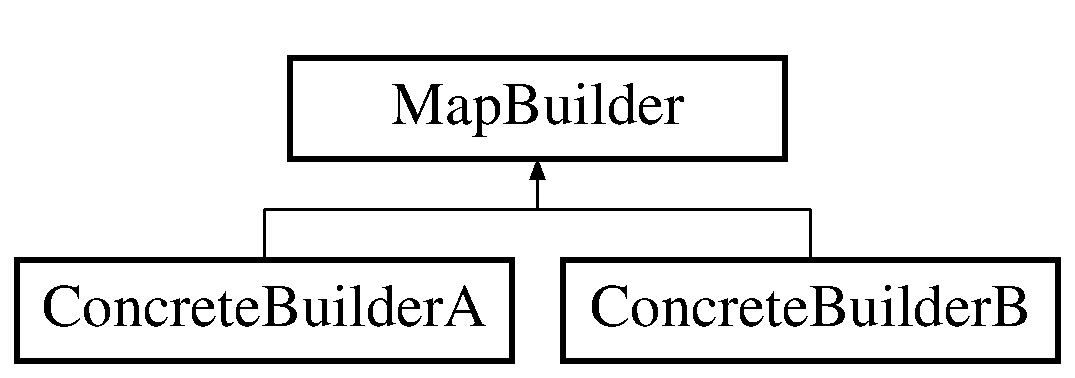
\includegraphics[height=2.000000cm]{class_map_builder}
\end{center}
\end{figure}
\subsection*{Public Member Functions}
\begin{DoxyCompactItemize}
\item 
\hypertarget{class_map_builder_a15fd21ef4019954fd7a09c6c6d33de34}{}\label{class_map_builder_a15fd21ef4019954fd7a09c6c6d33de34} 
virtual void {\bfseries build\+Character} (char, int, int, \hyperlink{class_map_object}{Map\+Object} $\ast$)=0
\item 
\hypertarget{class_map_builder_a7c95f41ce6057ca116298837bb11795d}{}\label{class_map_builder_a7c95f41ce6057ca116298837bb11795d} 
virtual void {\bfseries build\+Container} (int, int, vector$<$ \hyperlink{class_item}{Item} $\ast$$>$ \&)=0
\item 
\hyperlink{class_map}{Map} $\ast$ \hyperlink{class_map_builder_a6ea698affc46e8fab291eaf7b3ae8547}{get\+Map} ()
\item 
void \hyperlink{class_map_builder_aa8a9483778deb9083c5704b557adefdd}{set\+Map} (\hyperlink{class_map}{Map} $\ast$m)
\item 
void \hyperlink{class_map_builder_a6d61977f2e49d1113c37352249f808c7}{set\+Player\+Level} (int player\+Level)
\end{DoxyCompactItemize}
\subsection*{Protected Attributes}
\begin{DoxyCompactItemize}
\item 
\hypertarget{class_map_builder_a92d737b9ed6aeb247ac5cf9b3f226f70}{}\label{class_map_builder_a92d737b9ed6aeb247ac5cf9b3f226f70} 
\hyperlink{class_map}{Map} $\ast$ {\bfseries map}
\item 
\hypertarget{class_map_builder_a8850fe2b8a73585561fd7ffcaef76555}{}\label{class_map_builder_a8850fe2b8a73585561fd7ffcaef76555} 
int {\bfseries player\+Level}
\end{DoxyCompactItemize}


\subsection{Detailed Description}
Class for the implementation of a \hyperlink{class_map_builder}{Map\+Builder}. 

\subsection{Member Function Documentation}
\hypertarget{class_map_builder_a6ea698affc46e8fab291eaf7b3ae8547}{}\label{class_map_builder_a6ea698affc46e8fab291eaf7b3ae8547} 
\index{Map\+Builder@{Map\+Builder}!get\+Map@{get\+Map}}
\index{get\+Map@{get\+Map}!Map\+Builder@{Map\+Builder}}
\subsubsection{\texorpdfstring{get\+Map()}{getMap()}}
{\footnotesize\ttfamily \hyperlink{class_map}{Map}$\ast$ Map\+Builder\+::get\+Map (\begin{DoxyParamCaption}{ }\end{DoxyParamCaption})\hspace{0.3cm}{\ttfamily [inline]}}

Method to get map return A pointer to a map \hypertarget{class_map_builder_aa8a9483778deb9083c5704b557adefdd}{}\label{class_map_builder_aa8a9483778deb9083c5704b557adefdd} 
\index{Map\+Builder@{Map\+Builder}!set\+Map@{set\+Map}}
\index{set\+Map@{set\+Map}!Map\+Builder@{Map\+Builder}}
\subsubsection{\texorpdfstring{set\+Map()}{setMap()}}
{\footnotesize\ttfamily void Map\+Builder\+::set\+Map (\begin{DoxyParamCaption}\item[{\hyperlink{class_map}{Map} $\ast$}]{m }\end{DoxyParamCaption})\hspace{0.3cm}{\ttfamily [inline]}}

Method to set a map 
\begin{DoxyParams}{Parameters}
{\em m} & \+: Pointer to a map \\
\hline
\end{DoxyParams}
\hypertarget{class_map_builder_a6d61977f2e49d1113c37352249f808c7}{}\label{class_map_builder_a6d61977f2e49d1113c37352249f808c7} 
\index{Map\+Builder@{Map\+Builder}!set\+Player\+Level@{set\+Player\+Level}}
\index{set\+Player\+Level@{set\+Player\+Level}!Map\+Builder@{Map\+Builder}}
\subsubsection{\texorpdfstring{set\+Player\+Level()}{setPlayerLevel()}}
{\footnotesize\ttfamily void Map\+Builder\+::set\+Player\+Level (\begin{DoxyParamCaption}\item[{int}]{player\+Level }\end{DoxyParamCaption})\hspace{0.3cm}{\ttfamily [inline]}}

method to set the level of a player 
\begin{DoxyParams}{Parameters}
{\em player\+Level} & \+: level of player \\
\hline
\end{DoxyParams}


The documentation for this class was generated from the following file\+:\begin{DoxyCompactItemize}
\item 
\hyperlink{_map_builder_8h}{Map\+Builder.\+h}\end{DoxyCompactItemize}

\hypertarget{class_map_editor}{}\section{Map\+Editor Class Reference}
\label{class_map_editor}\index{Map\+Editor@{Map\+Editor}}
\subsection*{Public Member Functions}
\begin{DoxyCompactItemize}
\item 
\hypertarget{class_map_editor_a293c325d0b53afcf3924f006cdf60363}{}\label{class_map_editor_a293c325d0b53afcf3924f006cdf60363} 
\hyperlink{class_map_editor_a293c325d0b53afcf3924f006cdf60363}{Map\+Editor} ()
\begin{DoxyCompactList}\small\item\em Default constructor for the \hyperlink{class_map_editor}{Map\+Editor} class. \end{DoxyCompactList}\item 
void \hyperlink{class_map_editor_a57870586b534b4fe8057d629ee367651}{new\+Map} (int mapX, int mapY)
\item 
int \hyperlink{class_map_editor_a9ba798e6bed9b9ccad9176e39a776c31}{get\+Map\+SizeX} ()
\item 
int \hyperlink{class_map_editor_a2f538a32e1f2de6f1ddd224e17838ec5}{get\+Map\+SizeY} ()
\item 
void \hyperlink{class_map_editor_a2cec645bc70378aa8523dc8b61abc6a9}{set\+Tile} (int x, int y, \hyperlink{class_map_object}{Map\+Object} $\ast$object)
\item 
char \hyperlink{class_map_editor_a9fee49a6d578b6f39766c4ed46707770}{get\+Tile} (int x, int y)
\item 
string \hyperlink{class_map_editor_a8aae2a9a39abc032084926d3bfa69980}{get\+Available\+Map} (int index)
\item 
\hypertarget{class_map_editor_aeb40daa3d6ab846255a07dc987447c9b}{}\label{class_map_editor_aeb40daa3d6ab846255a07dc987447c9b} 
void \hyperlink{class_map_editor_aeb40daa3d6ab846255a07dc987447c9b}{set\+Available\+Maps} ()
\begin{DoxyCompactList}\small\item\em Implementation of set\+Available\+Maps to set all the available maps in the available\+Maps vector. \end{DoxyCompactList}\item 
int \hyperlink{class_map_editor_a5bd8ac96b712380197b274de67bbb81e}{get\+Available\+Maps\+Size} ()
\item 
bool \hyperlink{class_map_editor_a00a6d6fe02c11f0aa9a4a8f844f1437a}{load\+Map} (string map\+Name)
\item 
void \hyperlink{class_map_editor_ac1e3e9bab1f285d9055b6cc610fa9114}{save\+Map} (string map\+Name)
\end{DoxyCompactItemize}


\subsection{Member Function Documentation}
\hypertarget{class_map_editor_a8aae2a9a39abc032084926d3bfa69980}{}\label{class_map_editor_a8aae2a9a39abc032084926d3bfa69980} 
\index{Map\+Editor@{Map\+Editor}!get\+Available\+Map@{get\+Available\+Map}}
\index{get\+Available\+Map@{get\+Available\+Map}!Map\+Editor@{Map\+Editor}}
\subsubsection{\texorpdfstring{get\+Available\+Map()}{getAvailableMap()}}
{\footnotesize\ttfamily string Map\+Editor\+::get\+Available\+Map (\begin{DoxyParamCaption}\item[{int}]{index }\end{DoxyParamCaption})}

Implementation of get\+Available\+Map to get a specific saved map 
\begin{DoxyParams}{Parameters}
{\em index} & \+: an integer value of the position of the map in the array \\
\hline
\end{DoxyParams}
\begin{DoxyReturn}{Returns}
\+: a string representing the name of the map 
\end{DoxyReturn}
\hypertarget{class_map_editor_a5bd8ac96b712380197b274de67bbb81e}{}\label{class_map_editor_a5bd8ac96b712380197b274de67bbb81e} 
\index{Map\+Editor@{Map\+Editor}!get\+Available\+Maps\+Size@{get\+Available\+Maps\+Size}}
\index{get\+Available\+Maps\+Size@{get\+Available\+Maps\+Size}!Map\+Editor@{Map\+Editor}}
\subsubsection{\texorpdfstring{get\+Available\+Maps\+Size()}{getAvailableMapsSize()}}
{\footnotesize\ttfamily int Map\+Editor\+::get\+Available\+Maps\+Size (\begin{DoxyParamCaption}{ }\end{DoxyParamCaption})}

Implementation of get\+Available\+Maps\+Size to get the number of maps available \begin{DoxyReturn}{Returns}
\+: an integer representing the size of the map 
\end{DoxyReturn}
\hypertarget{class_map_editor_a9ba798e6bed9b9ccad9176e39a776c31}{}\label{class_map_editor_a9ba798e6bed9b9ccad9176e39a776c31} 
\index{Map\+Editor@{Map\+Editor}!get\+Map\+SizeX@{get\+Map\+SizeX}}
\index{get\+Map\+SizeX@{get\+Map\+SizeX}!Map\+Editor@{Map\+Editor}}
\subsubsection{\texorpdfstring{get\+Map\+Size\+X()}{getMapSizeX()}}
{\footnotesize\ttfamily int Map\+Editor\+::get\+Map\+SizeX (\begin{DoxyParamCaption}{ }\end{DoxyParamCaption})}

Implementation of get\+Map\+SizeX to get the map\textquotesingle{}s size in X \begin{DoxyReturn}{Returns}
\+: an integer value representing the the size of the map in x axis 
\end{DoxyReturn}
\hypertarget{class_map_editor_a2f538a32e1f2de6f1ddd224e17838ec5}{}\label{class_map_editor_a2f538a32e1f2de6f1ddd224e17838ec5} 
\index{Map\+Editor@{Map\+Editor}!get\+Map\+SizeY@{get\+Map\+SizeY}}
\index{get\+Map\+SizeY@{get\+Map\+SizeY}!Map\+Editor@{Map\+Editor}}
\subsubsection{\texorpdfstring{get\+Map\+Size\+Y()}{getMapSizeY()}}
{\footnotesize\ttfamily int Map\+Editor\+::get\+Map\+SizeY (\begin{DoxyParamCaption}{ }\end{DoxyParamCaption})}

Implementation of get\+Map\+SizeX to get the map\textquotesingle{}s size in Y \begin{DoxyReturn}{Returns}
\+: an integer value representing the the size of the map in y axis 
\end{DoxyReturn}
\hypertarget{class_map_editor_a9fee49a6d578b6f39766c4ed46707770}{}\label{class_map_editor_a9fee49a6d578b6f39766c4ed46707770} 
\index{Map\+Editor@{Map\+Editor}!get\+Tile@{get\+Tile}}
\index{get\+Tile@{get\+Tile}!Map\+Editor@{Map\+Editor}}
\subsubsection{\texorpdfstring{get\+Tile()}{getTile()}}
{\footnotesize\ttfamily char Map\+Editor\+::get\+Tile (\begin{DoxyParamCaption}\item[{int}]{x,  }\item[{int}]{y }\end{DoxyParamCaption})}

Implementation of get\+Tile to get a specific tile 
\begin{DoxyParams}{Parameters}
{\em x} & \+: an integer value for the horizontal position \\
\hline
{\em y} & \+: an integer value for the vertical position \\
\hline
\end{DoxyParams}
\begin{DoxyReturn}{Returns}
\+: a char value for the tile type 
\end{DoxyReturn}
\hypertarget{class_map_editor_a00a6d6fe02c11f0aa9a4a8f844f1437a}{}\label{class_map_editor_a00a6d6fe02c11f0aa9a4a8f844f1437a} 
\index{Map\+Editor@{Map\+Editor}!load\+Map@{load\+Map}}
\index{load\+Map@{load\+Map}!Map\+Editor@{Map\+Editor}}
\subsubsection{\texorpdfstring{load\+Map()}{loadMap()}}
{\footnotesize\ttfamily bool Map\+Editor\+::load\+Map (\begin{DoxyParamCaption}\item[{string}]{map\+Name }\end{DoxyParamCaption})}

Implementation of load\+Map to load a previously saved map 
\begin{DoxyParams}{Parameters}
{\em map\+Name} & \+: string representation the name of the map \\
\hline
\end{DoxyParams}
\hypertarget{class_map_editor_a57870586b534b4fe8057d629ee367651}{}\label{class_map_editor_a57870586b534b4fe8057d629ee367651} 
\index{Map\+Editor@{Map\+Editor}!new\+Map@{new\+Map}}
\index{new\+Map@{new\+Map}!Map\+Editor@{Map\+Editor}}
\subsubsection{\texorpdfstring{new\+Map()}{newMap()}}
{\footnotesize\ttfamily void Map\+Editor\+::new\+Map (\begin{DoxyParamCaption}\item[{int}]{mapX,  }\item[{int}]{mapY }\end{DoxyParamCaption})}

Implementation of new\+Map to create a new map 
\begin{DoxyParams}{Parameters}
{\em x} & \+: an integer value of the size in x axis of the map \\
\hline
{\em y} & \+: an integer value of the size in y axis of the map \\
\hline
\end{DoxyParams}
\hypertarget{class_map_editor_ac1e3e9bab1f285d9055b6cc610fa9114}{}\label{class_map_editor_ac1e3e9bab1f285d9055b6cc610fa9114} 
\index{Map\+Editor@{Map\+Editor}!save\+Map@{save\+Map}}
\index{save\+Map@{save\+Map}!Map\+Editor@{Map\+Editor}}
\subsubsection{\texorpdfstring{save\+Map()}{saveMap()}}
{\footnotesize\ttfamily void Map\+Editor\+::save\+Map (\begin{DoxyParamCaption}\item[{string}]{map\+Name }\end{DoxyParamCaption})}

Implementation of save\+Map to save the map as a binary file 
\begin{DoxyParams}{Parameters}
{\em map\+Name} & \+: name of the map to save \\
\hline
\end{DoxyParams}
\hypertarget{class_map_editor_a2cec645bc70378aa8523dc8b61abc6a9}{}\label{class_map_editor_a2cec645bc70378aa8523dc8b61abc6a9} 
\index{Map\+Editor@{Map\+Editor}!set\+Tile@{set\+Tile}}
\index{set\+Tile@{set\+Tile}!Map\+Editor@{Map\+Editor}}
\subsubsection{\texorpdfstring{set\+Tile()}{setTile()}}
{\footnotesize\ttfamily void Map\+Editor\+::set\+Tile (\begin{DoxyParamCaption}\item[{int}]{x,  }\item[{int}]{y,  }\item[{\hyperlink{class_map_object}{Map\+Object} $\ast$}]{object }\end{DoxyParamCaption})}

Implementation of set\+Tile to modifiy a map\textquotesingle{}s tile 
\begin{DoxyParams}{Parameters}
{\em x} & \+: an integer value for the horizontal position \\
\hline
{\em y} & \+: an integer value for the vertical position \\
\hline
{\em object} & \+: a char value for the tile type \\
\hline
\end{DoxyParams}


The documentation for this class was generated from the following files\+:\begin{DoxyCompactItemize}
\item 
\hyperlink{_map_editor_8h}{Map\+Editor.\+h}\item 
\hyperlink{_map_editor_8cpp}{Map\+Editor.\+cpp}\end{DoxyCompactItemize}

\hypertarget{class_map_object}{}\section{Map\+Object Class Reference}
\label{class_map_object}\index{Map\+Object@{Map\+Object}}


Class for the implementation of a superclass which consists of all objects that can be added onto the map.  




{\ttfamily \#include $<$Map\+Object.\+h$>$}

Inheritance diagram for Map\+Object\+:\begin{figure}[H]
\begin{center}
\leavevmode
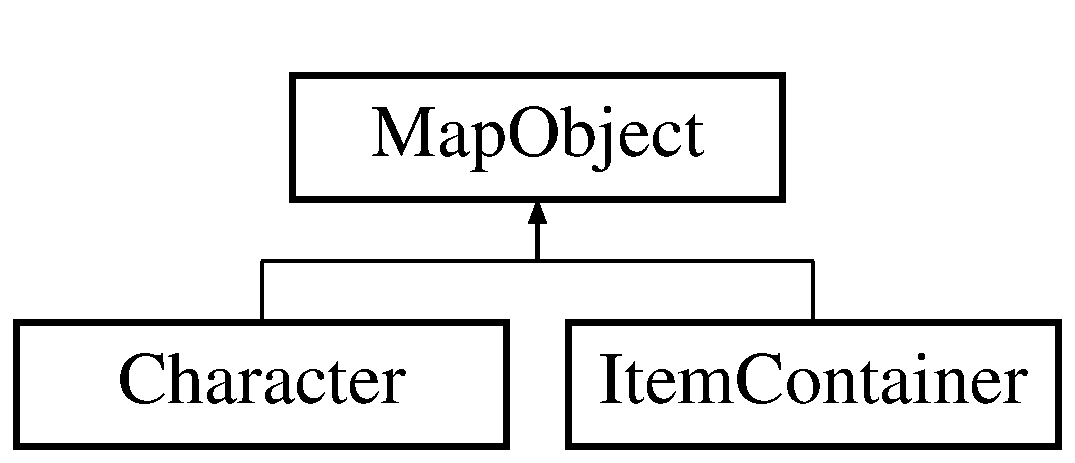
\includegraphics[height=2.000000cm]{class_map_object}
\end{center}
\end{figure}
\subsection*{Public Member Functions}
\begin{DoxyCompactItemize}
\item 
\hypertarget{class_map_object_a568754515cc72ce0861d30c3040d26d2}{}\label{class_map_object_a568754515cc72ce0861d30c3040d26d2} 
\hyperlink{class_map_object_a568754515cc72ce0861d30c3040d26d2}{Map\+Object} ()
\begin{DoxyCompactList}\small\item\em Default constructor. \end{DoxyCompactList}\item 
\hyperlink{class_map_object_a6d1c6e3754501b52af5a79a3322f0fba}{Map\+Object} (char type)
\item 
char \hyperlink{class_map_object_af740b1d1e4c4bbdb8727eeadcea0d008}{get\+Object\+Type} ()
\item 
void \hyperlink{class_map_object_a8a0fb292fa5e3262f304baeaa5db39fc}{set\+Object\+Type} (char type)
\end{DoxyCompactItemize}
\subsection*{Protected Attributes}
\begin{DoxyCompactItemize}
\item 
\hypertarget{class_map_object_ae39a5ef412aa349b2e9b329fad940b2d}{}\label{class_map_object_ae39a5ef412aa349b2e9b329fad940b2d} 
char {\bfseries object\+Type}
\end{DoxyCompactItemize}
\subsection*{Friends}
\begin{DoxyCompactItemize}
\item 
class \hyperlink{class_map_object_ac98d07dd8f7b70e16ccb9a01abf56b9c}{boost\+::serialization\+::access}
\end{DoxyCompactItemize}


\subsection{Detailed Description}
Class for the implementation of a superclass which consists of all objects that can be added onto the map. 

\subsection{Constructor \& Destructor Documentation}
\hypertarget{class_map_object_a6d1c6e3754501b52af5a79a3322f0fba}{}\label{class_map_object_a6d1c6e3754501b52af5a79a3322f0fba} 
\index{Map\+Object@{Map\+Object}!Map\+Object@{Map\+Object}}
\index{Map\+Object@{Map\+Object}!Map\+Object@{Map\+Object}}
\subsubsection{\texorpdfstring{Map\+Object()}{MapObject()}}
{\footnotesize\ttfamily Map\+Object\+::\+Map\+Object (\begin{DoxyParamCaption}\item[{char}]{type }\end{DoxyParamCaption})}

Constructor 
\begin{DoxyParams}{Parameters}
{\em type} & \+: Type of the object on the map as a char value \\
\hline
\end{DoxyParams}


\subsection{Member Function Documentation}
\hypertarget{class_map_object_af740b1d1e4c4bbdb8727eeadcea0d008}{}\label{class_map_object_af740b1d1e4c4bbdb8727eeadcea0d008} 
\index{Map\+Object@{Map\+Object}!get\+Object\+Type@{get\+Object\+Type}}
\index{get\+Object\+Type@{get\+Object\+Type}!Map\+Object@{Map\+Object}}
\subsubsection{\texorpdfstring{get\+Object\+Type()}{getObjectType()}}
{\footnotesize\ttfamily char Map\+Object\+::get\+Object\+Type (\begin{DoxyParamCaption}{ }\end{DoxyParamCaption})}

Method to obtain the type of the map object \begin{DoxyReturn}{Returns}
A map object type as a char value 
\end{DoxyReturn}
\hypertarget{class_map_object_a8a0fb292fa5e3262f304baeaa5db39fc}{}\label{class_map_object_a8a0fb292fa5e3262f304baeaa5db39fc} 
\index{Map\+Object@{Map\+Object}!set\+Object\+Type@{set\+Object\+Type}}
\index{set\+Object\+Type@{set\+Object\+Type}!Map\+Object@{Map\+Object}}
\subsubsection{\texorpdfstring{set\+Object\+Type()}{setObjectType()}}
{\footnotesize\ttfamily void Map\+Object\+::set\+Object\+Type (\begin{DoxyParamCaption}\item[{char}]{type }\end{DoxyParamCaption})}

set the type of an object 
\begin{DoxyParams}{Parameters}
{\em type} & \+: Type of the object on the map as a char value \\
\hline
\end{DoxyParams}


\subsection{Friends And Related Function Documentation}
\hypertarget{class_map_object_ac98d07dd8f7b70e16ccb9a01abf56b9c}{}\label{class_map_object_ac98d07dd8f7b70e16ccb9a01abf56b9c} 
\index{Map\+Object@{Map\+Object}!boost\+::serialization\+::access@{boost\+::serialization\+::access}}
\index{boost\+::serialization\+::access@{boost\+::serialization\+::access}!Map\+Object@{Map\+Object}}
\subsubsection{\texorpdfstring{boost\+::serialization\+::access}{boost::serialization::access}}
{\footnotesize\ttfamily friend class boost\+::serialization\+::access\hspace{0.3cm}{\ttfamily [friend]}}

Serialization When the class Archive corresponds to an output archive, the \& operator is defined similar to $<$$<$. Likewise, when the class Archive is a type of input archive the \& operator is defined similar to $>$$>$. 

The documentation for this class was generated from the following files\+:\begin{DoxyCompactItemize}
\item 
\hyperlink{_map_object_8h}{Map\+Object.\+h}\item 
\hyperlink{_map_object_8cpp}{Map\+Object.\+cpp}\end{DoxyCompactItemize}

\hypertarget{class_map_play}{}\section{Map\+Play Class Reference}
\label{class_map_play}\index{Map\+Play@{Map\+Play}}
Inheritance diagram for Map\+Play\+:\begin{figure}[H]
\begin{center}
\leavevmode
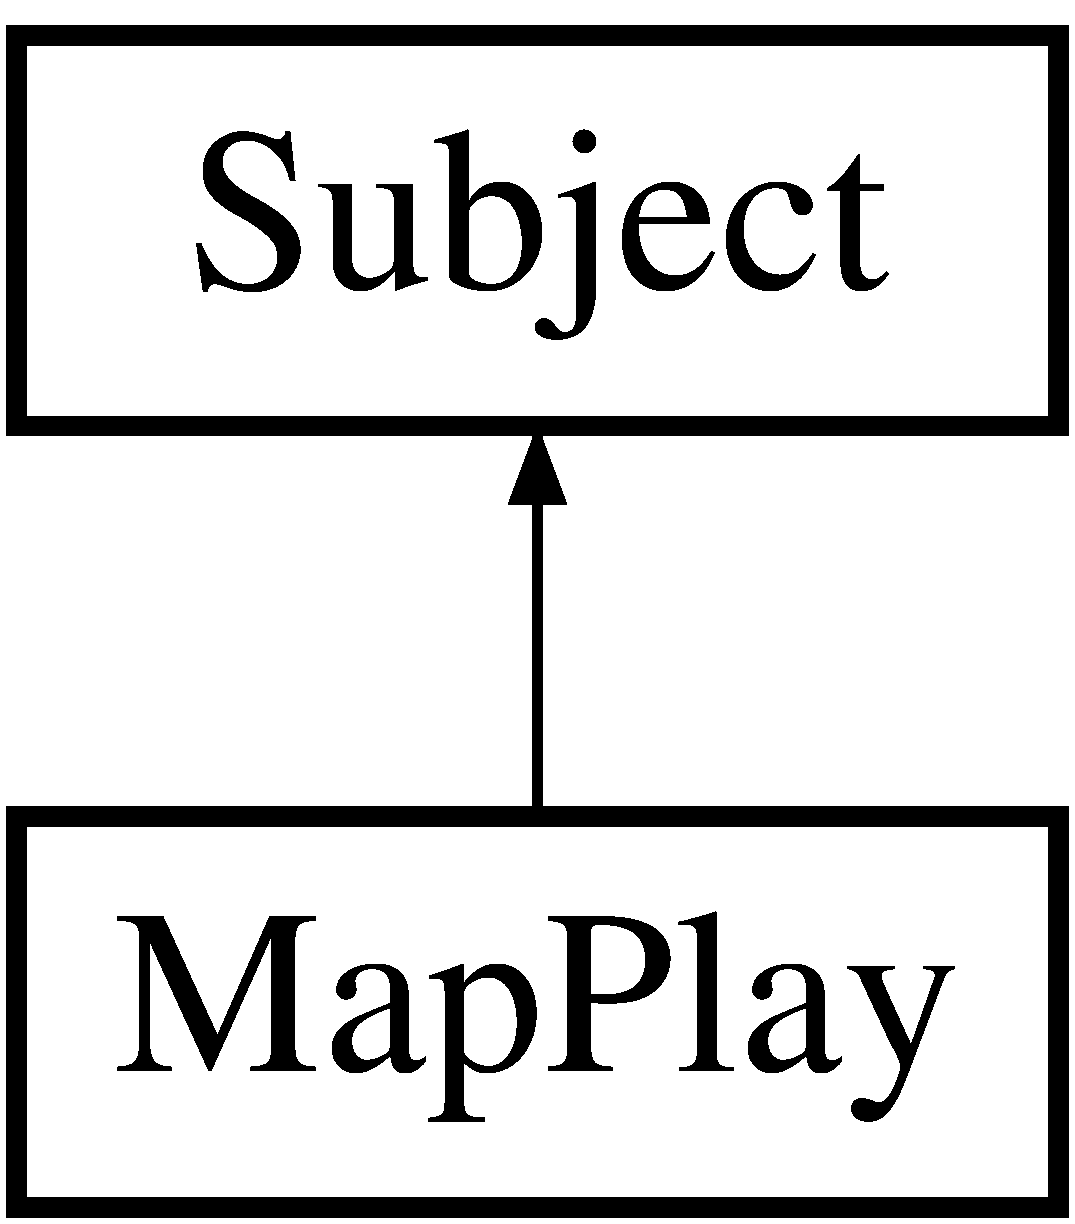
\includegraphics[height=2.000000cm]{class_map_play}
\end{center}
\end{figure}
\subsection*{Public Member Functions}
\begin{DoxyCompactItemize}
\item 
\hypertarget{class_map_play_a8028a7859349b4736abc9d3488e872ba}{}\label{class_map_play_a8028a7859349b4736abc9d3488e872ba} 
\hyperlink{class_map_play_a8028a7859349b4736abc9d3488e872ba}{Map\+Play} ()
\begin{DoxyCompactList}\small\item\em default constructor creates a map \end{DoxyCompactList}\item 
\hypertarget{class_map_play_ab24335073097f350d1890ad21b634da0}{}\label{class_map_play_ab24335073097f350d1890ad21b634da0} 
\hyperlink{class_map_play_ab24335073097f350d1890ad21b634da0}{$\sim$\+Map\+Play} ()
\begin{DoxyCompactList}\small\item\em default destructor \end{DoxyCompactList}\item 
void \hyperlink{class_map_play_a1f9b85a315373ef67846db347f6d4adc}{fill\+Cell} (int row, int col)
\begin{DoxyCompactList}\small\item\em method to modify a cell of the map \end{DoxyCompactList}\item 
\hypertarget{class_map_play_ad967902d8ff8cd582f81808acca41003}{}\label{class_map_play_ad967902d8ff8cd582f81808acca41003} 
char {\bfseries getc\+Map} (int row, int col)
\end{DoxyCompactItemize}


\subsection{Member Function Documentation}
\hypertarget{class_map_play_a1f9b85a315373ef67846db347f6d4adc}{}\label{class_map_play_a1f9b85a315373ef67846db347f6d4adc} 
\index{Map\+Play@{Map\+Play}!fill\+Cell@{fill\+Cell}}
\index{fill\+Cell@{fill\+Cell}!Map\+Play@{Map\+Play}}
\subsubsection{\texorpdfstring{fill\+Cell()}{fillCell()}}
{\footnotesize\ttfamily void Map\+Play\+::fill\+Cell (\begin{DoxyParamCaption}\item[{int}]{row,  }\item[{int}]{col }\end{DoxyParamCaption})}



method to modify a cell of the map 

The Observable object notifies all its registered observers 

The documentation for this class was generated from the following files\+:\begin{DoxyCompactItemize}
\item 
\hyperlink{_map_play_8h}{Map\+Play.\+h}\item 
\hyperlink{_map_play_8cpp}{Map\+Play.\+cpp}\end{DoxyCompactItemize}

\hypertarget{class_observer}{}\section{Observer Class Reference}
\label{class_observer}\index{Observer@{Observer}}


Abstract class that implements an \hyperlink{class_observer}{Observer}.  




{\ttfamily \#include $<$Observer.\+h$>$}

Inheritance diagram for Observer\+:\begin{figure}[H]
\begin{center}
\leavevmode
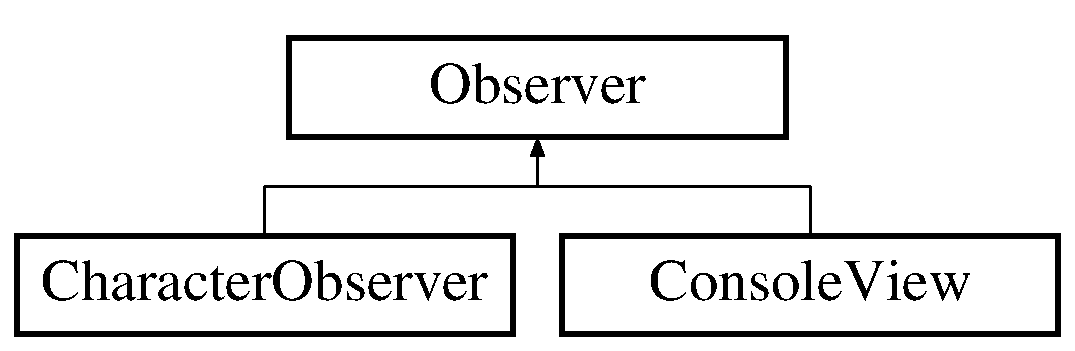
\includegraphics[height=2.000000cm]{class_observer}
\end{center}
\end{figure}
\subsection*{Public Member Functions}
\begin{DoxyCompactItemize}
\item 
\hypertarget{class_observer_a450645e61c136826f09940a1334c7f34}{}\label{class_observer_a450645e61c136826f09940a1334c7f34} 
\hyperlink{class_observer_a450645e61c136826f09940a1334c7f34}{$\sim$\+Observer} ()
\begin{DoxyCompactList}\small\item\em \hyperlink{class_observer}{Observer} destructor. \end{DoxyCompactList}\item 
\hypertarget{class_observer_a3c7c1dd5ca0f7bdb0e05098d1b7aac41}{}\label{class_observer_a3c7c1dd5ca0f7bdb0e05098d1b7aac41} 
virtual void {\bfseries Update} ()=0
\end{DoxyCompactItemize}
\subsection*{Protected Member Functions}
\begin{DoxyCompactItemize}
\item 
\hypertarget{class_observer_a19c43f80a38a332a6f694783df3c9835}{}\label{class_observer_a19c43f80a38a332a6f694783df3c9835} 
\hyperlink{class_observer_a19c43f80a38a332a6f694783df3c9835}{Observer} ()
\begin{DoxyCompactList}\small\item\em Default constructor for \hyperlink{class_observer}{Observer}. \end{DoxyCompactList}\end{DoxyCompactItemize}


\subsection{Detailed Description}
Abstract class that implements an \hyperlink{class_observer}{Observer}. 

The documentation for this class was generated from the following files\+:\begin{DoxyCompactItemize}
\item 
\hyperlink{_observer_8h}{Observer.\+h}\item 
\hyperlink{_observer_8cpp}{Observer.\+cpp}\end{DoxyCompactItemize}

\hypertarget{class_play}{}\section{Play Class Reference}
\label{class_play}\index{Play@{Play}}
\subsection*{Public Member Functions}
\begin{DoxyCompactItemize}
\item 
bool \hyperlink{class_play_afcc4c4ace55020c22c5a1568bd8de2fe}{load\+Campaign} (string campaign\+Name)
\item 
\hyperlink{class_map}{Map} $\ast$ \hyperlink{class_play_ac80f55229f24dce5473a3eef9ba35cb0}{get\+Campaign\+Map} (int index)
\item 
\hypertarget{class_play_ae4affe2e28c2377ee56406d297d2e113}{}\label{class_play_ae4affe2e28c2377ee56406d297d2e113} 
int {\bfseries get\+Available\+Campaigns\+Size} ()
\item 
\hypertarget{class_play_adfb9e21780d5bbd912d21cdcb50c158b}{}\label{class_play_adfb9e21780d5bbd912d21cdcb50c158b} 
void \hyperlink{class_play_adfb9e21780d5bbd912d21cdcb50c158b}{set\+Available\+Campaigns} ()
\begin{DoxyCompactList}\small\item\em Implementation of set\+Available\+Campaigns to set all the available campaigns in the available\+Campaigns vector. \end{DoxyCompactList}\item 
\hypertarget{class_play_a933fe6feb1eea405dd281fb0016c8d05}{}\label{class_play_a933fe6feb1eea405dd281fb0016c8d05} 
void {\bfseries set\+Available\+Characters} ()
\item 
string \hyperlink{class_play_a6b634b628eae6bf5af028b5e3c3f7c8b}{get\+Available\+Campaigns} (int index)
\item 
\hypertarget{class_play_a7d1891dd5a4f8754dbdc43cc1b8c3e0d}{}\label{class_play_a7d1891dd5a4f8754dbdc43cc1b8c3e0d} 
bool \hyperlink{class_play_a7d1891dd5a4f8754dbdc43cc1b8c3e0d}{load\+Maps} ()
\begin{DoxyCompactList}\small\item\em Implementation of load\+Maps to load all the maps of the campaign into campaign\+Maps. \end{DoxyCompactList}\item 
\hypertarget{class_play_a4f870d9bd33ec050c8695ef81466eb22}{}\label{class_play_a4f870d9bd33ec050c8695ef81466eb22} 
bool {\bfseries load\+Character} (string character\+Name)
\item 
\hypertarget{class_play_ad3beef5861eb27b6b79ee31ae1e08504}{}\label{class_play_ad3beef5861eb27b6b79ee31ae1e08504} 
int {\bfseries get\+Available\+Characters\+Size} ()
\item 
\hypertarget{class_play_abdaadd10c199a1cb3c3c9ab936701122}{}\label{class_play_abdaadd10c199a1cb3c3c9ab936701122} 
int {\bfseries get\+Campaign\+Size} ()
\item 
\hypertarget{class_play_a1eb9d18fd63ae2e2ac53187c20aab9aa}{}\label{class_play_a1eb9d18fd63ae2e2ac53187c20aab9aa} 
string {\bfseries get\+Available\+Characters} (int index)
\item 
\hypertarget{class_play_a249b82b8bb5928f598e2f9ebbfe50caf}{}\label{class_play_a249b82b8bb5928f598e2f9ebbfe50caf} 
void {\bfseries create\+New\+Character} ()
\item 
\hypertarget{class_play_a160b15f0f0e1390c650dadc8af52cdb2}{}\label{class_play_a160b15f0f0e1390c650dadc8af52cdb2} 
bool {\bfseries save\+Character} (string)
\item 
\hypertarget{class_play_ad7a55235bc6f657fda288549e2a840ee}{}\label{class_play_ad7a55235bc6f657fda288549e2a840ee} 
void {\bfseries modify\+Equipment} ()
\item 
\hypertarget{class_play_ae32a5c6b3a2e2e30722a523a5da78705}{}\label{class_play_ae32a5c6b3a2e2e30722a523a5da78705} 
void {\bfseries place\+Character\+On\+Map} (\hyperlink{class_map}{Map} $\ast$map)
\item 
\hypertarget{class_play_ab205e0f453258c40f2b2897c40d6bed9}{}\label{class_play_ab205e0f453258c40f2b2897c40d6bed9} 
bool {\bfseries move\+Character} (\hyperlink{class_map}{Map} $\ast$map, char direction)
\item 
\hypertarget{class_play_a67fc2a01a6d1777b1abeae01e830885f}{}\label{class_play_a67fc2a01a6d1777b1abeae01e830885f} 
void {\bfseries adapt\+Map\+To\+Player} (\hyperlink{class_map}{Map} $\ast$map)
\item 
\hypertarget{class_play_a5bc71c7d9cf9669928178501a74b8bcb}{}\label{class_play_a5bc71c7d9cf9669928178501a74b8bcb} 
void {\bfseries level\+Up\+Character} ()
\item 
\hypertarget{class_play_a0cd74f6325ddd8b1a1c9793e3f955d59}{}\label{class_play_a0cd74f6325ddd8b1a1c9793e3f955d59} 
void {\bfseries set\+Current\+Map} (int)
\item 
\hypertarget{class_play_a9a9dfca95eed4cab3fafae5308ccb59c}{}\label{class_play_a9a9dfca95eed4cab3fafae5308ccb59c} 
int {\bfseries get\+Current\+Map} ()
\item 
\hypertarget{class_play_a01a981cbef93cde2829f004b98b1d576}{}\label{class_play_a01a981cbef93cde2829f004b98b1d576} 
void {\bfseries set\+Map\+Builder} (\hyperlink{class_map_builder}{Map\+Builder} $\ast$)
\end{DoxyCompactItemize}


\subsection{Member Function Documentation}
\hypertarget{class_play_a6b634b628eae6bf5af028b5e3c3f7c8b}{}\label{class_play_a6b634b628eae6bf5af028b5e3c3f7c8b} 
\index{Play@{Play}!get\+Available\+Campaigns@{get\+Available\+Campaigns}}
\index{get\+Available\+Campaigns@{get\+Available\+Campaigns}!Play@{Play}}
\subsubsection{\texorpdfstring{get\+Available\+Campaigns()}{getAvailableCampaigns()}}
{\footnotesize\ttfamily string Play\+::get\+Available\+Campaigns (\begin{DoxyParamCaption}\item[{int}]{index }\end{DoxyParamCaption})}

Implementation of get\+Available\+Campaigns to get a specific saved campaign 
\begin{DoxyParams}{Parameters}
{\em index} & \+: an integer value of the position of the campaign in the vector \\
\hline
\end{DoxyParams}
\begin{DoxyReturn}{Returns}
\+: a string representing the name of the campaign 
\end{DoxyReturn}
\hypertarget{class_play_ac80f55229f24dce5473a3eef9ba35cb0}{}\label{class_play_ac80f55229f24dce5473a3eef9ba35cb0} 
\index{Play@{Play}!get\+Campaign\+Map@{get\+Campaign\+Map}}
\index{get\+Campaign\+Map@{get\+Campaign\+Map}!Play@{Play}}
\subsubsection{\texorpdfstring{get\+Campaign\+Map()}{getCampaignMap()}}
{\footnotesize\ttfamily \hyperlink{class_map}{Map} $\ast$ Play\+::get\+Campaign\+Map (\begin{DoxyParamCaption}\item[{int}]{index }\end{DoxyParamCaption})}

Implementation of get\+Campaign\+Map to get a specific map from a campaign 
\begin{DoxyParams}{Parameters}
{\em index} & \+: an integer value of the position of the map in the campaign vector \\
\hline
\end{DoxyParams}
\begin{DoxyReturn}{Returns}
\+: a map object at the specified position 
\end{DoxyReturn}
\hypertarget{class_play_afcc4c4ace55020c22c5a1568bd8de2fe}{}\label{class_play_afcc4c4ace55020c22c5a1568bd8de2fe} 
\index{Play@{Play}!load\+Campaign@{load\+Campaign}}
\index{load\+Campaign@{load\+Campaign}!Play@{Play}}
\subsubsection{\texorpdfstring{load\+Campaign()}{loadCampaign()}}
{\footnotesize\ttfamily bool Play\+::load\+Campaign (\begin{DoxyParamCaption}\item[{string}]{campaign\+Name }\end{DoxyParamCaption})}

Implementation of load\+Campaign to load the specified campaign into the campaign object  \+: a string value representing the name of the campaign 

The documentation for this class was generated from the following files\+:\begin{DoxyCompactItemize}
\item 
\hyperlink{_play_8h}{Play.\+h}\item 
\hyperlink{_play_8cpp}{Play.\+cpp}\end{DoxyCompactItemize}

\hypertarget{class_play_g_u_i}{}\section{Play\+G\+UI Class Reference}
\label{class_play_g_u_i}\index{Play\+G\+UI@{Play\+G\+UI}}
\subsection*{Public Member Functions}
\begin{DoxyCompactItemize}
\item 
\hypertarget{class_play_g_u_i_affa959c79f69de91745f770ea2f57a95}{}\label{class_play_g_u_i_affa959c79f69de91745f770ea2f57a95} 
{\bfseries Play\+G\+UI} (sf\+::\+Render\+Window \&window)
\item 
\hypertarget{class_play_g_u_i_aa8e186a6e54bb6ca90cfc6f8b3998ea5}{}\label{class_play_g_u_i_aa8e186a6e54bb6ca90cfc6f8b3998ea5} 
void {\bfseries open\+Load\+Campaign\+Window} ()
\item 
\hypertarget{class_play_g_u_i_a4e67c64926638db74232eb1b529c5be1}{}\label{class_play_g_u_i_a4e67c64926638db74232eb1b529c5be1} 
void {\bfseries open\+Load\+Character\+Window} ()
\item 
\hypertarget{class_play_g_u_i_a2f8eb016e8db7d518eea79686197594c}{}\label{class_play_g_u_i_a2f8eb016e8db7d518eea79686197594c} 
void {\bfseries open\+Map\+View} ()
\item 
\hypertarget{class_play_g_u_i_a6fea8bd3bd17cf9ab51a980819ce65d1}{}\label{class_play_g_u_i_a6fea8bd3bd17cf9ab51a980819ce65d1} 
void {\bfseries Update} ()
\item 
\hypertarget{class_play_g_u_i_a223179fe171e8c98aead106007783c03}{}\label{class_play_g_u_i_a223179fe171e8c98aead106007783c03} 
void {\bfseries Display} ()
\item 
\hypertarget{class_play_g_u_i_aa0842eb3fdf4ca0cd8d6730049cb4cbb}{}\label{class_play_g_u_i_aa0842eb3fdf4ca0cd8d6730049cb4cbb} 
void {\bfseries Start} ()
\end{DoxyCompactItemize}


The documentation for this class was generated from the following files\+:\begin{DoxyCompactItemize}
\item 
\hyperlink{_play_g_u_i_8h}{Play\+G\+U\+I.\+h}\item 
\hyperlink{_play_g_u_i_8cpp}{Play\+G\+U\+I.\+cpp}\end{DoxyCompactItemize}

\hypertarget{class_resources}{}\section{Resources Class Reference}
\label{class_resources}\index{Resources@{Resources}}
\subsection*{Public Member Functions}
\begin{DoxyCompactItemize}
\item 
\hypertarget{class_resources_ab09435991b8c485f92e0aa1fd00828b9}{}\label{class_resources_ab09435991b8c485f92e0aa1fd00828b9} 
\hyperlink{class_resources_ab09435991b8c485f92e0aa1fd00828b9}{Resources} ()
\begin{DoxyCompactList}\small\item\em Implementation of the default constructor of the \hyperlink{class_resources}{Resources} class. \end{DoxyCompactList}\item 
const sf\+::\+Texture \& \hyperlink{class_resources_a168468ac127f26c5d687ec6eceedda4f}{get\+Player\+Texture} ()
\item 
const sf\+::\+Texture \& \hyperlink{class_resources_af823e01e9f30b8a2070c23ba5c572113}{get\+Wall\+Texture} ()
\item 
const sf\+::\+Texture \& \hyperlink{class_resources_a575fd499564e6d905d7e08dfba1349e6}{get\+Treasure\+Texture} ()
\item 
const sf\+::\+Texture \& \hyperlink{class_resources_ae75ffa794e1d7f355ad4e2d8f01901ec}{get\+Ground\+Texture} ()
\item 
const sf\+::\+Texture \& \hyperlink{class_resources_a3715f3cd927d0b809556ea677b40092e}{get\+Door\+Texture} ()
\item 
const sf\+::\+Texture \& \hyperlink{class_resources_ad9ea9a040070bedc00927f00bf09242f}{get\+Enemy\+Texture} ()
\end{DoxyCompactItemize}


\subsection{Member Function Documentation}
\hypertarget{class_resources_a3715f3cd927d0b809556ea677b40092e}{}\label{class_resources_a3715f3cd927d0b809556ea677b40092e} 
\index{Resources@{Resources}!get\+Door\+Texture@{get\+Door\+Texture}}
\index{get\+Door\+Texture@{get\+Door\+Texture}!Resources@{Resources}}
\subsubsection{\texorpdfstring{get\+Door\+Texture()}{getDoorTexture()}}
{\footnotesize\ttfamily const sf\+::\+Texture \& Resources\+::get\+Door\+Texture (\begin{DoxyParamCaption}{ }\end{DoxyParamCaption})}

Implementation of get\+Door\+Texture to access the door\+Texture \begin{DoxyReturn}{Returns}
\+: a sf\+::\+Texture reference to the door texture 
\end{DoxyReturn}
\hypertarget{class_resources_ad9ea9a040070bedc00927f00bf09242f}{}\label{class_resources_ad9ea9a040070bedc00927f00bf09242f} 
\index{Resources@{Resources}!get\+Enemy\+Texture@{get\+Enemy\+Texture}}
\index{get\+Enemy\+Texture@{get\+Enemy\+Texture}!Resources@{Resources}}
\subsubsection{\texorpdfstring{get\+Enemy\+Texture()}{getEnemyTexture()}}
{\footnotesize\ttfamily const sf\+::\+Texture \& Resources\+::get\+Enemy\+Texture (\begin{DoxyParamCaption}{ }\end{DoxyParamCaption})}

Implementation of get\+Enemy\+Texture to access the enemy\+Texture \begin{DoxyReturn}{Returns}
\+: a sf\+::\+Texture reference to the enemy texture 
\end{DoxyReturn}
\hypertarget{class_resources_ae75ffa794e1d7f355ad4e2d8f01901ec}{}\label{class_resources_ae75ffa794e1d7f355ad4e2d8f01901ec} 
\index{Resources@{Resources}!get\+Ground\+Texture@{get\+Ground\+Texture}}
\index{get\+Ground\+Texture@{get\+Ground\+Texture}!Resources@{Resources}}
\subsubsection{\texorpdfstring{get\+Ground\+Texture()}{getGroundTexture()}}
{\footnotesize\ttfamily const sf\+::\+Texture \& Resources\+::get\+Ground\+Texture (\begin{DoxyParamCaption}{ }\end{DoxyParamCaption})}

Implementation of get\+Ground\+Texture to access the ground\+Texture \begin{DoxyReturn}{Returns}
\+: a sf\+::\+Texture reference to the ground texture 
\end{DoxyReturn}
\hypertarget{class_resources_a168468ac127f26c5d687ec6eceedda4f}{}\label{class_resources_a168468ac127f26c5d687ec6eceedda4f} 
\index{Resources@{Resources}!get\+Player\+Texture@{get\+Player\+Texture}}
\index{get\+Player\+Texture@{get\+Player\+Texture}!Resources@{Resources}}
\subsubsection{\texorpdfstring{get\+Player\+Texture()}{getPlayerTexture()}}
{\footnotesize\ttfamily const sf\+::\+Texture \& Resources\+::get\+Player\+Texture (\begin{DoxyParamCaption}{ }\end{DoxyParamCaption})}

Implementation of get\+Player\+Texture to access the player\+Texture \begin{DoxyReturn}{Returns}
\+: a sf\+::\+Texture reference to the player texture 
\end{DoxyReturn}
\hypertarget{class_resources_a575fd499564e6d905d7e08dfba1349e6}{}\label{class_resources_a575fd499564e6d905d7e08dfba1349e6} 
\index{Resources@{Resources}!get\+Treasure\+Texture@{get\+Treasure\+Texture}}
\index{get\+Treasure\+Texture@{get\+Treasure\+Texture}!Resources@{Resources}}
\subsubsection{\texorpdfstring{get\+Treasure\+Texture()}{getTreasureTexture()}}
{\footnotesize\ttfamily const sf\+::\+Texture \& Resources\+::get\+Treasure\+Texture (\begin{DoxyParamCaption}{ }\end{DoxyParamCaption})}

Implementation of get\+Treasure\+Texture to access the treasure\+Texture \begin{DoxyReturn}{Returns}
\+: a sf\+::\+Texture reference to the treasure texture 
\end{DoxyReturn}
\hypertarget{class_resources_af823e01e9f30b8a2070c23ba5c572113}{}\label{class_resources_af823e01e9f30b8a2070c23ba5c572113} 
\index{Resources@{Resources}!get\+Wall\+Texture@{get\+Wall\+Texture}}
\index{get\+Wall\+Texture@{get\+Wall\+Texture}!Resources@{Resources}}
\subsubsection{\texorpdfstring{get\+Wall\+Texture()}{getWallTexture()}}
{\footnotesize\ttfamily const sf\+::\+Texture \& Resources\+::get\+Wall\+Texture (\begin{DoxyParamCaption}{ }\end{DoxyParamCaption})}

Implementation of get\+Wall\+Texture to access the wall\+Texture \begin{DoxyReturn}{Returns}
\+: a sf\+::\+Texture reference to the wall texture 
\end{DoxyReturn}


The documentation for this class was generated from the following files\+:\begin{DoxyCompactItemize}
\item 
\hyperlink{_resources_8h}{Resources.\+h}\item 
\hyperlink{_resources_8cpp}{Resources.\+cpp}\end{DoxyCompactItemize}

\hypertarget{class_ring}{}\section{Ring Class Reference}
\label{class_ring}\index{Ring@{Ring}}


Class for the implementation of a ring.  




{\ttfamily \#include $<$Ring.\+h$>$}

Inheritance diagram for Ring\+:\begin{figure}[H]
\begin{center}
\leavevmode
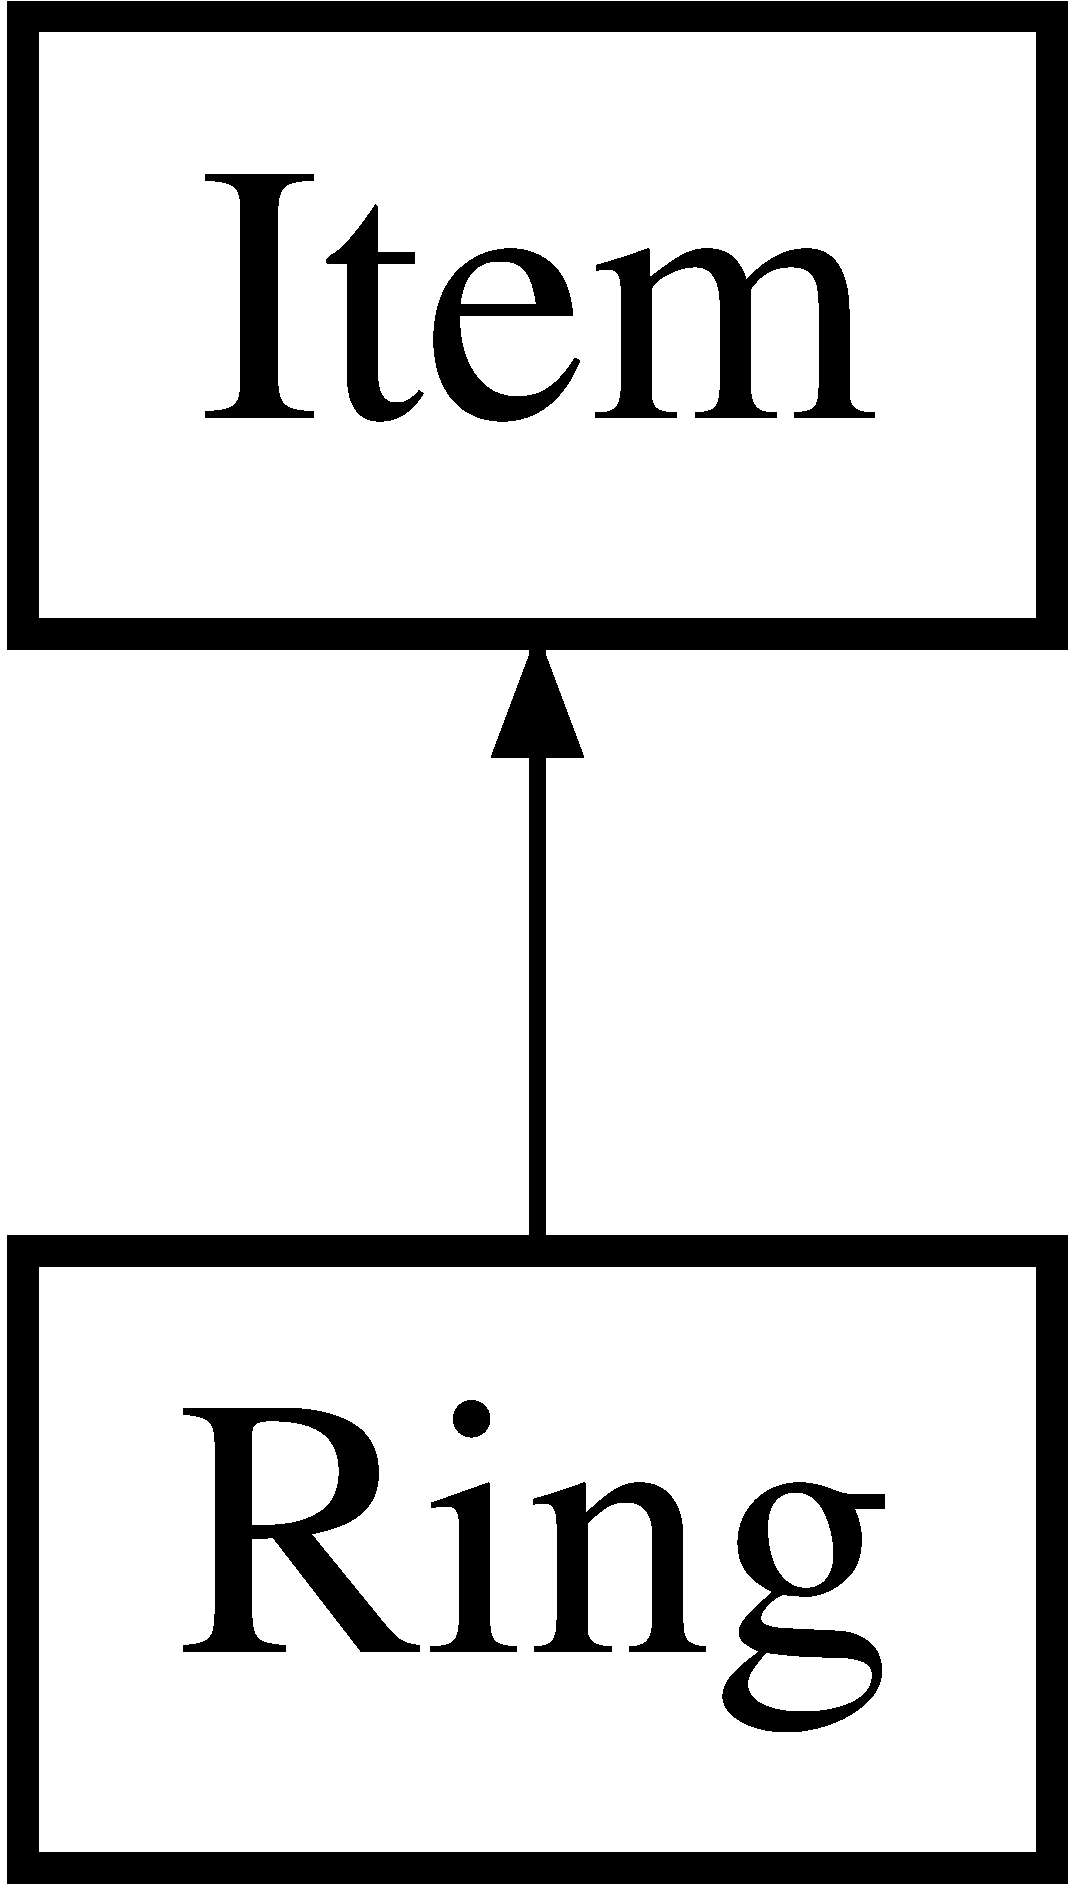
\includegraphics[height=2.000000cm]{class_ring}
\end{center}
\end{figure}
\subsection*{Public Member Functions}
\begin{DoxyCompactItemize}
\item 
\hypertarget{class_ring_afc47f40ab072db783126111b70693e49}{}\label{class_ring_afc47f40ab072db783126111b70693e49} 
\hyperlink{class_ring_afc47f40ab072db783126111b70693e49}{Ring} ()
\begin{DoxyCompactList}\small\item\em Default constructor. \end{DoxyCompactList}\item 
\hyperlink{class_ring_a029cccc4d2563fb2f9e85ab60d7e37d3}{Ring} (string name, int armor\+Class, int strength, int constitution, int wisdom, int charisma)
\item 
\hyperlink{class_ring_ae0295e0b34deab9238405440e62e1fb0}{Ring} (string name, vector$<$ \hyperlink{class_enhancement}{Enhancement} $>$ enhancements)
\item 
bool \hyperlink{class_ring_a9170e11e83f0a5b8443e9267e5bd6c8a}{validate\+Item} ()
\end{DoxyCompactItemize}
\subsection*{Friends}
\begin{DoxyCompactItemize}
\item 
\hypertarget{class_ring_ac98d07dd8f7b70e16ccb9a01abf56b9c}{}\label{class_ring_ac98d07dd8f7b70e16ccb9a01abf56b9c} 
class \hyperlink{class_ring_ac98d07dd8f7b70e16ccb9a01abf56b9c}{boost\+::serialization\+::access}
\begin{DoxyCompactList}\small\item\em serialization \end{DoxyCompactList}\end{DoxyCompactItemize}
\subsection*{Additional Inherited Members}


\subsection{Detailed Description}
Class for the implementation of a ring. 

\subsection{Constructor \& Destructor Documentation}
\hypertarget{class_ring_a029cccc4d2563fb2f9e85ab60d7e37d3}{}\label{class_ring_a029cccc4d2563fb2f9e85ab60d7e37d3} 
\index{Ring@{Ring}!Ring@{Ring}}
\index{Ring@{Ring}!Ring@{Ring}}
\subsubsection{\texorpdfstring{Ring()}{Ring()}\hspace{0.1cm}{\footnotesize\ttfamily [1/2]}}
{\footnotesize\ttfamily Ring\+::\+Ring (\begin{DoxyParamCaption}\item[{string}]{name,  }\item[{int}]{armor\+Class\+Bonus,  }\item[{int}]{strength\+Bonus,  }\item[{int}]{constitution\+Bonus,  }\item[{int}]{wisdom\+Bonus,  }\item[{int}]{charisma\+Bonus }\end{DoxyParamCaption})}

Constructor that calls an \hyperlink{class_item}{Item} constructor 
\begin{DoxyParams}{Parameters}
{\em name} & \+: Name of ring item \\
\hline
{\em armor\+Class\+Bonus} & \+: Integer representing the enhancement bonus for the stats \hyperlink{class_armor}{Armor} Class \\
\hline
{\em strength\+Bonus} & \+: Integer representing the enhancement bonus for the stats Strength \\
\hline
{\em constitution\+Bonus} & \+: Integer representing the enhancement bonus for the stats Constitution \\
\hline
{\em wisdom\+Bonus} & \+: Integer representing the enhancement bonus for the stats Wisdom \\
\hline
{\em charisma\+Bonus} & \+: Integer representing the enhancement bonus for the stats Charisma \\
\hline
\end{DoxyParams}
\hypertarget{class_ring_ae0295e0b34deab9238405440e62e1fb0}{}\label{class_ring_ae0295e0b34deab9238405440e62e1fb0} 
\index{Ring@{Ring}!Ring@{Ring}}
\index{Ring@{Ring}!Ring@{Ring}}
\subsubsection{\texorpdfstring{Ring()}{Ring()}\hspace{0.1cm}{\footnotesize\ttfamily [2/2]}}
{\footnotesize\ttfamily Ring\+::\+Ring (\begin{DoxyParamCaption}\item[{string}]{name,  }\item[{vector$<$ \hyperlink{class_enhancement}{Enhancement} $>$}]{enhancements }\end{DoxyParamCaption})}

Constructor taking a vector of enhancements as parameter 
\begin{DoxyParams}{Parameters}
{\em name} & \+: Name of items \\
\hline
{\em enhancements} & \+: Vector of enhancements \\
\hline
\end{DoxyParams}


\subsection{Member Function Documentation}
\hypertarget{class_ring_a9170e11e83f0a5b8443e9267e5bd6c8a}{}\label{class_ring_a9170e11e83f0a5b8443e9267e5bd6c8a} 
\index{Ring@{Ring}!validate\+Item@{validate\+Item}}
\index{validate\+Item@{validate\+Item}!Ring@{Ring}}
\subsubsection{\texorpdfstring{validate\+Item()}{validateItem()}}
{\footnotesize\ttfamily bool Ring\+::validate\+Item (\begin{DoxyParamCaption}{ }\end{DoxyParamCaption})\hspace{0.3cm}{\ttfamily [virtual]}}

Overrided method to validate that the armor only enhances \textquotesingle{}A\+R\+M\+OR C\+L\+A\+SS\textquotesingle{}, \textquotesingle{}S\+T\+R\+E\+N\+G\+TH\textquotesingle{}, \textquotesingle{}C\+O\+N\+S\+T\+I\+T\+U\+T\+I\+ON\textquotesingle{}, \textquotesingle{}W\+I\+S\+D\+OM\textquotesingle{} and \textquotesingle{}C\+H\+A\+R\+I\+S\+MA\textquotesingle{} and verify that the bonus values are within \mbox{[}1..5\mbox{]} \begin{DoxyReturn}{Returns}
True if the enhancement list is valid according to the rules, false if not 
\end{DoxyReturn}


Reimplemented from \hyperlink{class_item_a6603371b60aaded48f697975c81fc25b}{Item}.



The documentation for this class was generated from the following files\+:\begin{DoxyCompactItemize}
\item 
\hyperlink{_ring_8h}{Ring.\+h}\item 
\hyperlink{_ring_8cpp}{Ring.\+cpp}\end{DoxyCompactItemize}

\hypertarget{class_shield}{}\section{Shield Class Reference}
\label{class_shield}\index{Shield@{Shield}}


Class for the implementation of a shield.  




{\ttfamily \#include $<$Shield.\+h$>$}

Inheritance diagram for Shield\+:\begin{figure}[H]
\begin{center}
\leavevmode
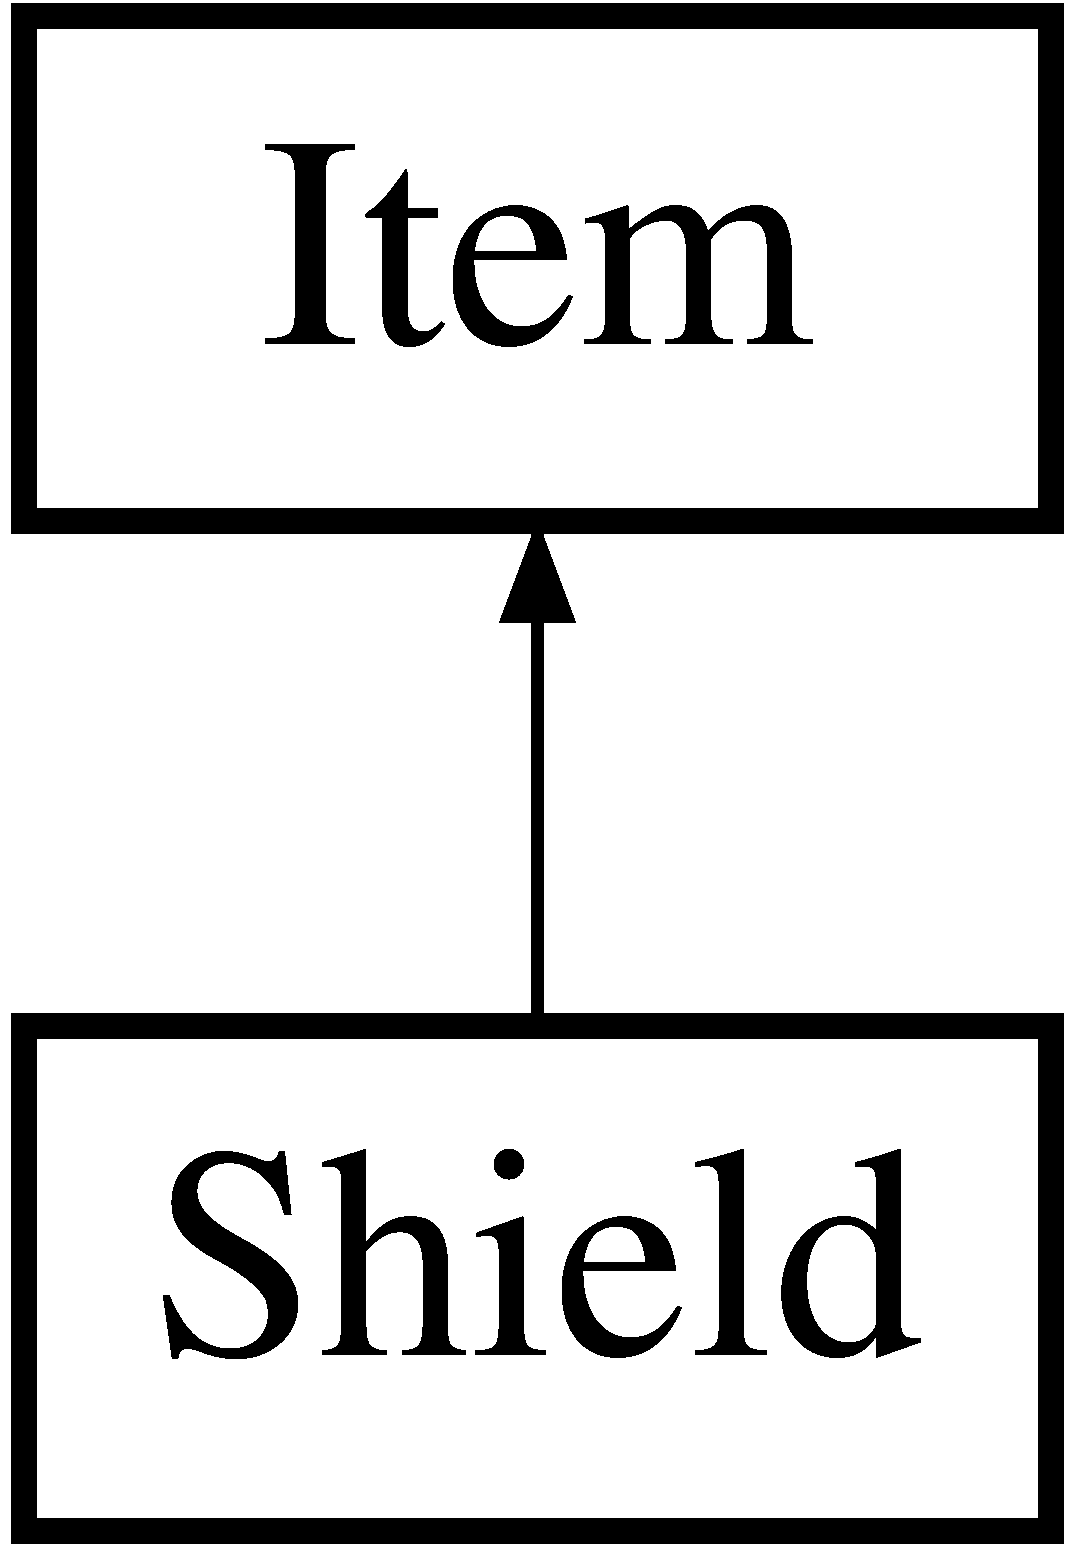
\includegraphics[height=2.000000cm]{class_shield}
\end{center}
\end{figure}
\subsection*{Public Member Functions}
\begin{DoxyCompactItemize}
\item 
\hypertarget{class_shield_a8a6e827c94750d8c1a1d523cb1b105de}{}\label{class_shield_a8a6e827c94750d8c1a1d523cb1b105de} 
\hyperlink{class_shield_a8a6e827c94750d8c1a1d523cb1b105de}{Shield} ()
\begin{DoxyCompactList}\small\item\em Default constructor. \end{DoxyCompactList}\item 
\hyperlink{class_shield_ab14292c5626c5f10a57e727ca298ee49}{Shield} (string name, int armor\+Class)
\item 
\hyperlink{class_shield_ad95eb094f4ed92a7f59694d9a5939565}{Shield} (string name, vector$<$ \hyperlink{class_enhancement}{Enhancement} $>$ enhancements)
\item 
bool \hyperlink{class_shield_af28f146ed96720bd007a62a5871cd206}{validate\+Item} ()
\end{DoxyCompactItemize}
\subsection*{Friends}
\begin{DoxyCompactItemize}
\item 
\hypertarget{class_shield_ac98d07dd8f7b70e16ccb9a01abf56b9c}{}\label{class_shield_ac98d07dd8f7b70e16ccb9a01abf56b9c} 
class \hyperlink{class_shield_ac98d07dd8f7b70e16ccb9a01abf56b9c}{boost\+::serialization\+::access}
\begin{DoxyCompactList}\small\item\em serialization \end{DoxyCompactList}\end{DoxyCompactItemize}
\subsection*{Additional Inherited Members}


\subsection{Detailed Description}
Class for the implementation of a shield. 

\subsection{Constructor \& Destructor Documentation}
\hypertarget{class_shield_ab14292c5626c5f10a57e727ca298ee49}{}\label{class_shield_ab14292c5626c5f10a57e727ca298ee49} 
\index{Shield@{Shield}!Shield@{Shield}}
\index{Shield@{Shield}!Shield@{Shield}}
\subsubsection{\texorpdfstring{Shield()}{Shield()}\hspace{0.1cm}{\footnotesize\ttfamily [1/2]}}
{\footnotesize\ttfamily Shield\+::\+Shield (\begin{DoxyParamCaption}\item[{string}]{name,  }\item[{int}]{armor\+Class\+Bonus }\end{DoxyParamCaption})}

Constructor that calls an \hyperlink{class_item}{Item} constructor 
\begin{DoxyParams}{Parameters}
{\em name} & \+: Name of shield item \\
\hline
{\em armor\+Class\+Bonus} & \+: Integer representing the enhancement bonus for the stats \hyperlink{class_armor}{Armor} Class \\
\hline
\end{DoxyParams}
\hypertarget{class_shield_ad95eb094f4ed92a7f59694d9a5939565}{}\label{class_shield_ad95eb094f4ed92a7f59694d9a5939565} 
\index{Shield@{Shield}!Shield@{Shield}}
\index{Shield@{Shield}!Shield@{Shield}}
\subsubsection{\texorpdfstring{Shield()}{Shield()}\hspace{0.1cm}{\footnotesize\ttfamily [2/2]}}
{\footnotesize\ttfamily Shield\+::\+Shield (\begin{DoxyParamCaption}\item[{string}]{name,  }\item[{vector$<$ \hyperlink{class_enhancement}{Enhancement} $>$}]{enhancements }\end{DoxyParamCaption})}

Constructor taking a vector of enhancements as parameter 
\begin{DoxyParams}{Parameters}
{\em name} & \+: Name of shield item \\
\hline
{\em enhancements} & \+: Vector of enhancements \\
\hline
\end{DoxyParams}


\subsection{Member Function Documentation}
\hypertarget{class_shield_af28f146ed96720bd007a62a5871cd206}{}\label{class_shield_af28f146ed96720bd007a62a5871cd206} 
\index{Shield@{Shield}!validate\+Item@{validate\+Item}}
\index{validate\+Item@{validate\+Item}!Shield@{Shield}}
\subsubsection{\texorpdfstring{validate\+Item()}{validateItem()}}
{\footnotesize\ttfamily bool Shield\+::validate\+Item (\begin{DoxyParamCaption}{ }\end{DoxyParamCaption})\hspace{0.3cm}{\ttfamily [virtual]}}

Overrided method to validate that the armor only enhances \textquotesingle{}A\+R\+M\+OR C\+L\+A\+SS\textquotesingle{} and verify that the bonus values are within \mbox{[}1..5\mbox{]} \begin{DoxyReturn}{Returns}
True if the enhancement list is valid according to the rules, false if not 
\end{DoxyReturn}


Reimplemented from \hyperlink{class_item_a6603371b60aaded48f697975c81fc25b}{Item}.



The documentation for this class was generated from the following files\+:\begin{DoxyCompactItemize}
\item 
\hyperlink{_shield_8h}{Shield.\+h}\item 
\hyperlink{_shield_8cpp}{Shield.\+cpp}\end{DoxyCompactItemize}

\hypertarget{class_subject}{}\section{Subject Class Reference}
\label{class_subject}\index{Subject@{Subject}}


Abstract class that implements a \hyperlink{class_subject}{Subject}.  




{\ttfamily \#include $<$Subject.\+h$>$}

Inheritance diagram for Subject\+:\begin{figure}[H]
\begin{center}
\leavevmode
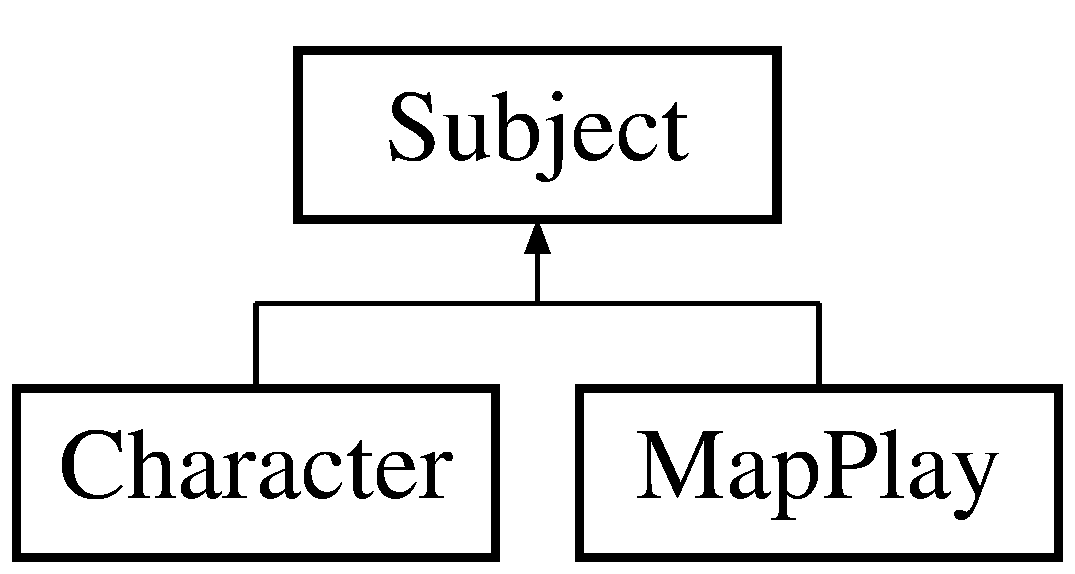
\includegraphics[height=2.000000cm]{class_subject}
\end{center}
\end{figure}
\subsection*{Public Member Functions}
\begin{DoxyCompactItemize}
\item 
\hyperlink{class_subject_ab468044832c824c6d6c2f46272655207}{Subject} ()
\item 
\hyperlink{class_subject_a7c4f522850f718466e5be7eb55ba1969}{$\sim$\+Subject} ()
\item 
virtual void \hyperlink{class_subject_a4178d3cef008c713370791c6578334de}{Attach} (\hyperlink{class_observer}{Observer} $\ast$o)
\item 
virtual void \hyperlink{class_subject_ac839596fe840efb970e36a66554e3095}{Detach} (\hyperlink{class_observer}{Observer} $\ast$o)
\item 
\hypertarget{class_subject_afdf01736ff099d286543b450d96215f1}{}\label{class_subject_afdf01736ff099d286543b450d96215f1} 
virtual void \hyperlink{class_subject_afdf01736ff099d286543b450d96215f1}{Notify} ()
\begin{DoxyCompactList}\small\item\em Notify function that triggers an update for every observer that is attached to the subject. \end{DoxyCompactList}\item 
int \hyperlink{class_subject_a606f81da175e7ba807ed72482e4435bf}{get\+Number\+Observers} ()
\end{DoxyCompactItemize}


\subsection{Detailed Description}
Abstract class that implements a \hyperlink{class_subject}{Subject}. 

\subsection{Constructor \& Destructor Documentation}
\hypertarget{class_subject_ab468044832c824c6d6c2f46272655207}{}\label{class_subject_ab468044832c824c6d6c2f46272655207} 
\index{Subject@{Subject}!Subject@{Subject}}
\index{Subject@{Subject}!Subject@{Subject}}
\subsubsection{\texorpdfstring{Subject()}{Subject()}}
{\footnotesize\ttfamily Subject\+::\+Subject (\begin{DoxyParamCaption}{ }\end{DoxyParamCaption})}

Default constructor for \hyperlink{class_subject}{Subject} On instantiation, creates a new list of observers as one subject can have many observers \hypertarget{class_subject_a7c4f522850f718466e5be7eb55ba1969}{}\label{class_subject_a7c4f522850f718466e5be7eb55ba1969} 
\index{Subject@{Subject}!````~Subject@{$\sim$\+Subject}}
\index{````~Subject@{$\sim$\+Subject}!Subject@{Subject}}
\subsubsection{\texorpdfstring{$\sim$\+Subject()}{~Subject()}}
{\footnotesize\ttfamily Subject\+::$\sim$\+Subject (\begin{DoxyParamCaption}{ }\end{DoxyParamCaption})}

Destructor for \hyperlink{class_subject}{Subject} When called, deletes the list of observers that was previously instantiated 

\subsection{Member Function Documentation}
\hypertarget{class_subject_a4178d3cef008c713370791c6578334de}{}\label{class_subject_a4178d3cef008c713370791c6578334de} 
\index{Subject@{Subject}!Attach@{Attach}}
\index{Attach@{Attach}!Subject@{Subject}}
\subsubsection{\texorpdfstring{Attach()}{Attach()}}
{\footnotesize\ttfamily void Subject\+::\+Attach (\begin{DoxyParamCaption}\item[{\hyperlink{class_observer}{Observer} $\ast$}]{o }\end{DoxyParamCaption})\hspace{0.3cm}{\ttfamily [virtual]}}

Attach function that attaches an observer to the subject 
\begin{DoxyParams}{Parameters}
{\em o} & Pointer to an object with supertype \hyperlink{class_observer}{Observer} \\
\hline
\end{DoxyParams}
\hypertarget{class_subject_ac839596fe840efb970e36a66554e3095}{}\label{class_subject_ac839596fe840efb970e36a66554e3095} 
\index{Subject@{Subject}!Detach@{Detach}}
\index{Detach@{Detach}!Subject@{Subject}}
\subsubsection{\texorpdfstring{Detach()}{Detach()}}
{\footnotesize\ttfamily void Subject\+::\+Detach (\begin{DoxyParamCaption}\item[{\hyperlink{class_observer}{Observer} $\ast$}]{o }\end{DoxyParamCaption})\hspace{0.3cm}{\ttfamily [virtual]}}

Detach function that removes observer referenced by the parameter from the list of the \hyperlink{class_subject}{Subject}\textquotesingle{}s observers 
\begin{DoxyParams}{Parameters}
{\em o} & Pointer to an object with supertype \hyperlink{class_observer}{Observer} \\
\hline
\end{DoxyParams}
\hypertarget{class_subject_a606f81da175e7ba807ed72482e4435bf}{}\label{class_subject_a606f81da175e7ba807ed72482e4435bf} 
\index{Subject@{Subject}!get\+Number\+Observers@{get\+Number\+Observers}}
\index{get\+Number\+Observers@{get\+Number\+Observers}!Subject@{Subject}}
\subsubsection{\texorpdfstring{get\+Number\+Observers()}{getNumberObservers()}}
{\footnotesize\ttfamily int Subject\+::get\+Number\+Observers (\begin{DoxyParamCaption}{ }\end{DoxyParamCaption})}

For debugging purposes, returns the number of observers attached to the calling subject return int, number of observers in the list of observers of a given subject 

The documentation for this class was generated from the following files\+:\begin{DoxyCompactItemize}
\item 
\hyperlink{_subject_8h}{Subject.\+h}\item 
\hyperlink{_subject_8cpp}{Subject.\+cpp}\end{DoxyCompactItemize}

\hypertarget{class_user_driven_editor}{}\section{User\+Driven\+Editor Class Reference}
\label{class_user_driven_editor}\index{User\+Driven\+Editor@{User\+Driven\+Editor}}
\subsection*{Static Public Member Functions}
\begin{DoxyCompactItemize}
\item 
\hypertarget{class_user_driven_editor_a3df8443432852b64259758491e121825}{}\label{class_user_driven_editor_a3df8443432852b64259758491e121825} 
static \hyperlink{class_item_container}{Item\+Container} $\ast$ {\bfseries create\+Chest} ()
\item 
\hypertarget{class_user_driven_editor_a493179a964f7c9b6798f9fdf6ed26ec6}{}\label{class_user_driven_editor_a493179a964f7c9b6798f9fdf6ed26ec6} 
static \hyperlink{class_character}{Character} $\ast$ {\bfseries create\+Character} ()
\end{DoxyCompactItemize}


The documentation for this class was generated from the following files\+:\begin{DoxyCompactItemize}
\item 
\hyperlink{_user_driven_editor_8h}{User\+Driven\+Editor.\+h}\item 
\hyperlink{_user_driven_editor_8cpp}{User\+Driven\+Editor.\+cpp}\end{DoxyCompactItemize}

\hypertarget{class_weapon}{}\section{Weapon Class Reference}
\label{class_weapon}\index{Weapon@{Weapon}}


Class for the implementation of a weapon.  




{\ttfamily \#include $<$Weapon.\+h$>$}

Inheritance diagram for Weapon\+:\begin{figure}[H]
\begin{center}
\leavevmode
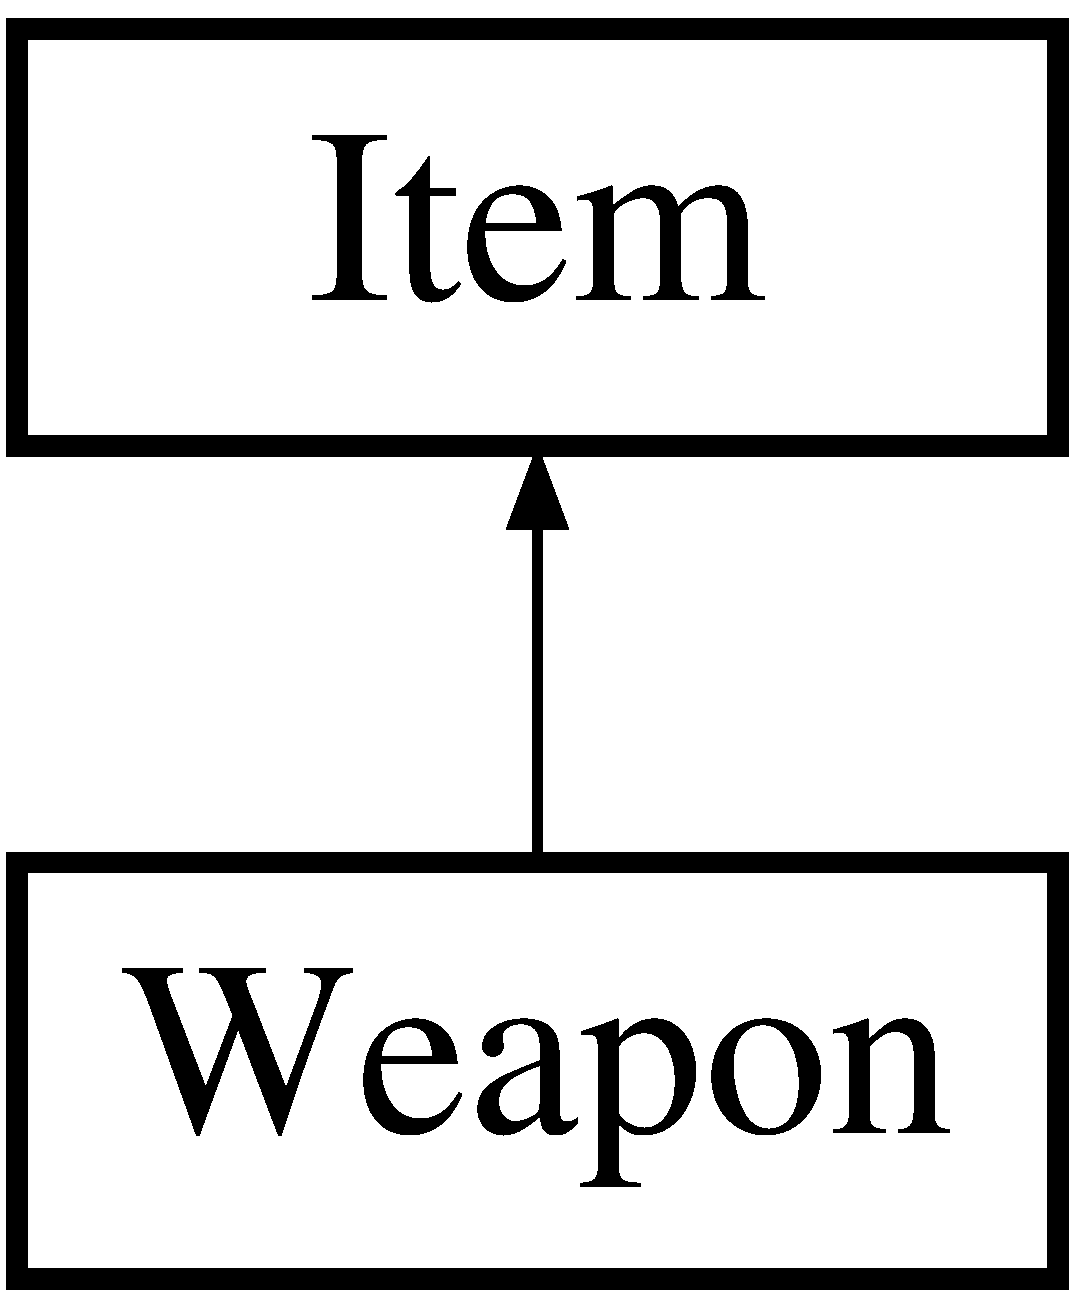
\includegraphics[height=2.000000cm]{class_weapon}
\end{center}
\end{figure}
\subsection*{Public Member Functions}
\begin{DoxyCompactItemize}
\item 
\hypertarget{class_weapon_a42dbc46dd70319a24763992c4ebbd396}{}\label{class_weapon_a42dbc46dd70319a24763992c4ebbd396} 
\hyperlink{class_weapon_a42dbc46dd70319a24763992c4ebbd396}{Weapon} ()
\begin{DoxyCompactList}\small\item\em Default constructor. \end{DoxyCompactList}\item 
\hyperlink{class_weapon_ad3c6f6756018c1c3ad316aaa26aae972}{Weapon} (string name, int attack\+Bonus, int damage\+Bonus)
\item 
\hyperlink{class_weapon_aa713aefb98583e759336a4d8338bfbcf}{Weapon} (string name, vector$<$ \hyperlink{class_enhancement}{Enhancement} $>$ enhancements)
\item 
bool \hyperlink{class_weapon_afa7ce016c3cba686399cbe57628f8c70}{validate\+Item} ()
\end{DoxyCompactItemize}
\subsection*{Friends}
\begin{DoxyCompactItemize}
\item 
\hypertarget{class_weapon_ac98d07dd8f7b70e16ccb9a01abf56b9c}{}\label{class_weapon_ac98d07dd8f7b70e16ccb9a01abf56b9c} 
class \hyperlink{class_weapon_ac98d07dd8f7b70e16ccb9a01abf56b9c}{boost\+::serialization\+::access}
\begin{DoxyCompactList}\small\item\em serialization \end{DoxyCompactList}\end{DoxyCompactItemize}
\subsection*{Additional Inherited Members}


\subsection{Detailed Description}
Class for the implementation of a weapon. 

\subsection{Constructor \& Destructor Documentation}
\hypertarget{class_weapon_ad3c6f6756018c1c3ad316aaa26aae972}{}\label{class_weapon_ad3c6f6756018c1c3ad316aaa26aae972} 
\index{Weapon@{Weapon}!Weapon@{Weapon}}
\index{Weapon@{Weapon}!Weapon@{Weapon}}
\subsubsection{\texorpdfstring{Weapon()}{Weapon()}\hspace{0.1cm}{\footnotesize\ttfamily [1/2]}}
{\footnotesize\ttfamily Weapon\+::\+Weapon (\begin{DoxyParamCaption}\item[{string}]{name,  }\item[{int}]{attack\+Value,  }\item[{int}]{damage\+Value }\end{DoxyParamCaption})}

Constructor that calls an \hyperlink{class_item}{Item} constructor 
\begin{DoxyParams}{Parameters}
{\em name} & \+: Name of weapon item \\
\hline
{\em attack\+Value} & \+: Integer representing the enhancement bonus for the stats Attack bonus \\
\hline
{\em damage\+Value} & \+: Integer representing the enhancement bonus for the stats Damage bonus \\
\hline
\end{DoxyParams}
\hypertarget{class_weapon_aa713aefb98583e759336a4d8338bfbcf}{}\label{class_weapon_aa713aefb98583e759336a4d8338bfbcf} 
\index{Weapon@{Weapon}!Weapon@{Weapon}}
\index{Weapon@{Weapon}!Weapon@{Weapon}}
\subsubsection{\texorpdfstring{Weapon()}{Weapon()}\hspace{0.1cm}{\footnotesize\ttfamily [2/2]}}
{\footnotesize\ttfamily Weapon\+::\+Weapon (\begin{DoxyParamCaption}\item[{string}]{name,  }\item[{vector$<$ \hyperlink{class_enhancement}{Enhancement} $>$}]{enhancements }\end{DoxyParamCaption})}

Constructor taking a vector of enhancements as parameter 
\begin{DoxyParams}{Parameters}
{\em name} & \+: Name of weapon item \\
\hline
{\em enhancements} & \+: Vector of enhancements \\
\hline
\end{DoxyParams}


\subsection{Member Function Documentation}
\hypertarget{class_weapon_afa7ce016c3cba686399cbe57628f8c70}{}\label{class_weapon_afa7ce016c3cba686399cbe57628f8c70} 
\index{Weapon@{Weapon}!validate\+Item@{validate\+Item}}
\index{validate\+Item@{validate\+Item}!Weapon@{Weapon}}
\subsubsection{\texorpdfstring{validate\+Item()}{validateItem()}}
{\footnotesize\ttfamily bool Weapon\+::validate\+Item (\begin{DoxyParamCaption}{ }\end{DoxyParamCaption})\hspace{0.3cm}{\ttfamily [virtual]}}

Overrided method to validate that the armor only enhances \textquotesingle{}A\+T\+T\+A\+CK B\+O\+N\+US\textquotesingle{} and \textquotesingle{}D\+A\+M\+A\+GE B\+O\+N\+US\textquotesingle{}and verify that the bonus values are within \mbox{[}1..5\mbox{]} \begin{DoxyReturn}{Returns}
True if the enhancement list is valid according to the rules, false if not 
\end{DoxyReturn}


Reimplemented from \hyperlink{class_item_a6603371b60aaded48f697975c81fc25b}{Item}.



The documentation for this class was generated from the following files\+:\begin{DoxyCompactItemize}
\item 
\hyperlink{_weapon_8h}{Weapon.\+h}\item 
\hyperlink{_weapon_8cpp}{Weapon.\+cpp}\end{DoxyCompactItemize}

\chapter{File Documentation}
\hypertarget{_armor_8cpp}{}\section{Armor.\+cpp File Reference}
\label{_armor_8cpp}\index{Armor.\+cpp@{Armor.\+cpp}}


Implementation file for the \hyperlink{class_armor}{Armor} class.  


{\ttfamily \#include \char`\"{}stdafx.\+h\char`\"{}}\newline
{\ttfamily \#include \char`\"{}Armor.\+h\char`\"{}}\newline


\subsection{Detailed Description}
Implementation file for the \hyperlink{class_armor}{Armor} class. 


\hypertarget{_armor_8h}{}\section{Armor.\+h File Reference}
\label{_armor_8h}\index{Armor.\+h@{Armor.\+h}}


Header file for the \hyperlink{class_armor}{Armor} class.  


{\ttfamily \#include \char`\"{}Item.\+h\char`\"{}}\newline
\subsection*{Classes}
\begin{DoxyCompactItemize}
\item 
class \hyperlink{class_armor}{Armor}
\begin{DoxyCompactList}\small\item\em Class for the implementation of an armor. \end{DoxyCompactList}\end{DoxyCompactItemize}


\subsection{Detailed Description}
Header file for the \hyperlink{class_armor}{Armor} class. 

This class represents a specific \hyperlink{class_item}{Item} type. It is a subclass of \hyperlink{class_item}{Item}. 
\hypertarget{_belt_8cpp}{}\section{Belt.\+cpp File Reference}
\label{_belt_8cpp}\index{Belt.\+cpp@{Belt.\+cpp}}


Implementation file for the \hyperlink{class_armor}{Armor} class.  


{\ttfamily \#include \char`\"{}stdafx.\+h\char`\"{}}\newline
{\ttfamily \#include \char`\"{}Belt.\+h\char`\"{}}\newline


\subsection{Detailed Description}
Implementation file for the \hyperlink{class_armor}{Armor} class. 


\hypertarget{_belt_8h}{}\section{Belt.\+h File Reference}
\label{_belt_8h}\index{Belt.\+h@{Belt.\+h}}


Header file for the \hyperlink{class_belt}{Belt} class.  


{\ttfamily \#include \char`\"{}Item.\+h\char`\"{}}\newline
\subsection*{Classes}
\begin{DoxyCompactItemize}
\item 
class \hyperlink{class_belt}{Belt}
\begin{DoxyCompactList}\small\item\em Class for the implementation of a belt. \end{DoxyCompactList}\end{DoxyCompactItemize}


\subsection{Detailed Description}
Header file for the \hyperlink{class_belt}{Belt} class. 


\hypertarget{_boots_8cpp}{}\section{Boots.\+cpp File Reference}
\label{_boots_8cpp}\index{Boots.\+cpp@{Boots.\+cpp}}


Implementation file for the \hyperlink{class_boots}{Boots} class.  


{\ttfamily \#include \char`\"{}stdafx.\+h\char`\"{}}\newline
{\ttfamily \#include \char`\"{}Boots.\+h\char`\"{}}\newline


\subsection{Detailed Description}
Implementation file for the \hyperlink{class_boots}{Boots} class. 


\hypertarget{_boots_8h}{}\section{Boots.\+h File Reference}
\label{_boots_8h}\index{Boots.\+h@{Boots.\+h}}


Header file for the \hyperlink{class_boots}{Boots} class.  


{\ttfamily \#include \char`\"{}Item.\+h\char`\"{}}\newline
\subsection*{Classes}
\begin{DoxyCompactItemize}
\item 
class \hyperlink{class_boots}{Boots}
\begin{DoxyCompactList}\small\item\em Class for the implementation of a boot. \end{DoxyCompactList}\end{DoxyCompactItemize}


\subsection{Detailed Description}
Header file for the \hyperlink{class_boots}{Boots} class. 


\hypertarget{_campaign_8h}{}\section{Campaign.\+h File Reference}
\label{_campaign_8h}\index{Campaign.\+h@{Campaign.\+h}}


Header file for the \hyperlink{class_campaign}{Campaign} The following class implements the campaign class according to the requirements. A vector of strings was used to identify the maps linked in the campaign The vector allows to load maps in order according to their specified path Vectors are dynamic and allow to add elements to it without knowning its size previously The library used to serialization of class is Boost.\+Serialization It was used because of its efficiency and portability. With Boost, it is possible to serialize and export a class into a binary data file.  


{\ttfamily \#include \char`\"{}Map.\+h\char`\"{}}\newline
{\ttfamily \#include $<$boost/serialization/serialization.\+hpp$>$}\newline
{\ttfamily \#include $<$boost/archive/binary\+\_\+oarchive.\+hpp$>$}\newline
{\ttfamily \#include $<$boost/archive/binary\+\_\+iarchive.\+hpp$>$}\newline
{\ttfamily \#include $<$boost/serialization/vector.\+hpp$>$}\newline
\subsection*{Classes}
\begin{DoxyCompactItemize}
\item 
class \hyperlink{class_campaign}{Campaign}
\end{DoxyCompactItemize}


\subsection{Detailed Description}
Header file for the \hyperlink{class_campaign}{Campaign} The following class implements the campaign class according to the requirements. A vector of strings was used to identify the maps linked in the campaign The vector allows to load maps in order according to their specified path Vectors are dynamic and allow to add elements to it without knowning its size previously The library used to serialization of class is Boost.\+Serialization It was used because of its efficiency and portability. With Boost, it is possible to serialize and export a class into a binary data file. 


\hypertarget{_campaign_editor_8cpp}{}\section{Campaign\+Editor.\+cpp File Reference}
\label{_campaign_editor_8cpp}\index{Campaign\+Editor.\+cpp@{Campaign\+Editor.\+cpp}}


Implementation file for \hyperlink{class_campaign_editor}{Campaign\+Editor} class.  


{\ttfamily \#include \char`\"{}stdafx.\+h\char`\"{}}\newline
{\ttfamily \#include \char`\"{}Campaign\+Editor.\+h\char`\"{}}\newline


\subsection{Detailed Description}
Implementation file for \hyperlink{class_campaign_editor}{Campaign\+Editor} class. 


\hypertarget{_campaign_editor_8h}{}\section{Campaign\+Editor.\+h File Reference}
\label{_campaign_editor_8h}\index{Campaign\+Editor.\+h@{Campaign\+Editor.\+h}}


Header file for the \hyperlink{class_campaign_editor}{Campaign\+Editor} class The following class implements the campaign editor according to the requirements. It allows a user to modify, and create maps The user can load previously created maps and save new ones The library used for serialization of classes is Boost.\+Serialization It was used because of its efficiency and portability. With Boost, it is possible to serialize and export a class into a binary data file.  


{\ttfamily \#include \char`\"{}Campaign.\+h\char`\"{}}\newline
{\ttfamily \#include $<$iostream$>$}\newline
{\ttfamily \#include $<$vector$>$}\newline
{\ttfamily \#include $<$fstream$>$}\newline
{\ttfamily \#include $<$boost/filesystem.\+hpp$>$}\newline
\subsection*{Classes}
\begin{DoxyCompactItemize}
\item 
class \hyperlink{class_campaign_editor}{Campaign\+Editor}
\end{DoxyCompactItemize}


\subsection{Detailed Description}
Header file for the \hyperlink{class_campaign_editor}{Campaign\+Editor} class The following class implements the campaign editor according to the requirements. It allows a user to modify, and create maps The user can load previously created maps and save new ones The library used for serialization of classes is Boost.\+Serialization It was used because of its efficiency and portability. With Boost, it is possible to serialize and export a class into a binary data file. 


\hypertarget{_character_8cpp}{}\section{Character.\+cpp File Reference}
\label{_character_8cpp}\index{Character.\+cpp@{Character.\+cpp}}


Implementation file for the \hyperlink{class_character}{Character} class.  


{\ttfamily \#include \char`\"{}stdafx.\+h\char`\"{}}\newline
{\ttfamily \#include \char`\"{}Character.\+h\char`\"{}}\newline
{\ttfamily \#include \char`\"{}Dice.\+h\char`\"{}}\newline
{\ttfamily \#include $<$stdlib.\+h$>$}\newline
{\ttfamily \#include $<$cstdlib$>$}\newline
{\ttfamily \#include $<$ctime$>$}\newline
{\ttfamily \#include $<$algorithm$>$}\newline
{\ttfamily \#include $<$functional$>$}\newline
{\ttfamily \#include $<$iostream$>$}\newline
{\ttfamily \#include $<$conio.\+h$>$}\newline
{\ttfamily \#include $<$windows.\+h$>$}\newline
{\ttfamily \#include $<$math.\+h$>$}\newline
{\ttfamily \#include $<$string$>$}\newline
{\ttfamily \#include $<$vector$>$}\newline


\subsection{Detailed Description}
Implementation file for the \hyperlink{class_character}{Character} class. 

Assumes that \hyperlink{class_character}{Character} is of fighter type 
\hypertarget{_character_8h}{}\section{Character.\+h File Reference}
\label{_character_8h}\index{Character.\+h@{Character.\+h}}


Header file for the \hyperlink{class_character}{Character} class.  


{\ttfamily \#include \char`\"{}Subject.\+h\char`\"{}}\newline
{\ttfamily \#include \char`\"{}Map\+Object.\+h\char`\"{}}\newline
{\ttfamily \#include \char`\"{}Item\+Container.\+h\char`\"{}}\newline
{\ttfamily \#include $<$string$>$}\newline
{\ttfamily \#include $<$boost/serialization/vector.\+hpp$>$}\newline
{\ttfamily \#include $<$boost/serialization/string.\+hpp$>$}\newline
\subsection*{Classes}
\begin{DoxyCompactItemize}
\item 
class \hyperlink{class_character}{Character}
\begin{DoxyCompactList}\small\item\em Class that implements a character. \end{DoxyCompactList}\end{DoxyCompactItemize}


\subsection{Detailed Description}
Header file for the \hyperlink{class_character}{Character} class. 

Game rules explained\+:
\begin{DoxyItemize}
\item To calculate character\textquotesingle{}s ability scores, 4 six-\/sided dice are rolled, where the highest 3 are kept and summed.
\item This is repeated 5 more times to have a total of 6 scores. They are distributed in the character\textquotesingle{}s ability scores based on the priorities for fighter class.
\item The priority is\+: Strength, Dexterity, Constitution, Charisma, Intelligence and Wisdom.
\item Then, to calculate the ability modifiers, we add 10 to the ability scores, divide by 2, and round down.
\item Initial hit points are found by having 10 summed with the character\textquotesingle{}s calculated constitution modifier.
\item At later levels, hit points are found by adding a d10 dice roll and the character\textquotesingle{}s constitution modifier to the previous hp.
\item \hyperlink{class_armor}{Armor} class depends on the type of armor worn, but for the constructor it is 11 + dexterity modifier.
\item Attack bonus depends on level, but for the constructor, attack bonus is just strength + dexterity modifiers.
\item Damage bonus is also dependant on level, but initially is is simply the strength modifier.
\end{DoxyItemize}

Design of assignment\+:
\begin{DoxyItemize}
\item The design of this program is that it is constituted of a \hyperlink{class_character}{Character} header file.
\item It also has the \hyperlink{class_character}{Character} cpp file which is the class definition of the \hyperlink{class_character}{Character} class.
\item \hyperlink{class_character}{Character} objects will be initialized by default to be of the fighter class, for the sake of the project.
\item There are also 2 test files, the Character\+Test header, and the corresponding Character\+Test cpp file.
\item They are the unit tests which validate major test cases of the functionalities of the program using C\+P\+P\+Unit framework.
\item Finally, there is the main function which runs either the test cases, or the driver to demonstrate the program.
\item (By default I have commented out the unit tests \hyperlink{_driver_8cpp_a0ddf1224851353fc92bfbff6f499fa97}{main()} function, simply uncomment them and comment the driver to view the unit tests).
\item \hyperlink{class_character}{Character} and \hyperlink{class_subject}{Subject} classes have been added for assignment 2, which are the abstract classes that make up the observer design pattern.
\item As \hyperlink{class_character}{Character} is the subject for this assignment, it inherits from the \hyperlink{class_subject}{Subject} class, while \hyperlink{class_character_observer}{Character\+Observer}, the observer class created, inherits from \hyperlink{class_observer}{Observer} class.
\end{DoxyItemize}

Libraries used\+:
\begin{DoxyItemize}
\item I have used many libraries to boost the performance and functionality of the program.
\item The iostream library is used to allow output to the console for viewing purposes.
\item The ctime and windows.\+h libraries were used to access the machine real time for the randomizer functions optimization.
\item math.\+h was used for the simple mathematics functions to avoid unecessary coding, such as the floor() function to round down a double.
\item string was included because objects of type string were used in the program to display the equipped items of the character.
\item And finally, for the driver, some C\+P\+P\+Unit libraries were included to perform and run the test cases 
\end{DoxyItemize}
\hypertarget{_character_observer_8cpp}{}\section{Character\+Observer.\+cpp File Reference}
\label{_character_observer_8cpp}\index{Character\+Observer.\+cpp@{Character\+Observer.\+cpp}}


Cpp file for \hyperlink{class_character_observer}{Character\+Observer} class.  


{\ttfamily \#include \char`\"{}stdafx.\+h\char`\"{}}\newline
{\ttfamily \#include \char`\"{}Character\+Observer.\+h\char`\"{}}\newline
{\ttfamily \#include \char`\"{}Observer.\+h\char`\"{}}\newline
{\ttfamily \#include $<$iostream$>$}\newline
{\ttfamily \#include $<$string$>$}\newline


\subsection{Detailed Description}
Cpp file for \hyperlink{class_character_observer}{Character\+Observer} class. 


\hypertarget{_character_observer_8h}{}\section{Character\+Observer.\+h File Reference}
\label{_character_observer_8h}\index{Character\+Observer.\+h@{Character\+Observer.\+h}}


Header file for \hyperlink{class_character_observer}{Character\+Observer} class.  


{\ttfamily \#include \char`\"{}Observer.\+h\char`\"{}}\newline
{\ttfamily \#include \char`\"{}Character.\+h\char`\"{}}\newline
\subsection*{Classes}
\begin{DoxyCompactItemize}
\item 
class \hyperlink{class_character_observer}{Character\+Observer}
\begin{DoxyCompactList}\small\item\em Class that inherits from \hyperlink{class_observer}{Observer} and that implements \hyperlink{class_character_observer}{Character\+Observer}. \end{DoxyCompactList}\end{DoxyCompactItemize}


\subsection{Detailed Description}
Header file for \hyperlink{class_character_observer}{Character\+Observer} class. 


\hypertarget{_concrete_builder_a_8cpp}{}\section{Concrete\+Builder\+A.\+cpp File Reference}
\label{_concrete_builder_a_8cpp}\index{Concrete\+Builder\+A.\+cpp@{Concrete\+Builder\+A.\+cpp}}


Implementation file for the \hyperlink{class_concrete_builder_a}{Concrete\+BuilderA} class.  


{\ttfamily \#include \char`\"{}Concrete\+Builder\+A.\+h\char`\"{}}\newline
{\ttfamily \#include \char`\"{}Character.\+h\char`\"{}}\newline
{\ttfamily \#include $<$fstream$>$}\newline
{\ttfamily \#include $<$iostream$>$}\newline
{\ttfamily \#include $<$string$>$}\newline


\subsection{Detailed Description}
Implementation file for the \hyperlink{class_concrete_builder_a}{Concrete\+BuilderA} class. 


\hypertarget{_concrete_builder_b_8cpp}{}\section{Concrete\+Builder\+B.\+cpp File Reference}
\label{_concrete_builder_b_8cpp}\index{Concrete\+Builder\+B.\+cpp@{Concrete\+Builder\+B.\+cpp}}


Implementation file for the \hyperlink{class_concrete_builder_b}{Concrete\+BuilderB} class.  


{\ttfamily \#include \char`\"{}Concrete\+Builder\+B.\+h\char`\"{}}\newline


\subsection{Detailed Description}
Implementation file for the \hyperlink{class_concrete_builder_b}{Concrete\+BuilderB} class. 


\hypertarget{_console_view_8cpp}{}\section{Console\+View.\+cpp File Reference}
\label{_console_view_8cpp}\index{Console\+View.\+cpp@{Console\+View.\+cpp}}


Implementation file for the \hyperlink{class_console_view}{Console\+View} class.  


{\ttfamily \#include \char`\"{}Console\+View.\+h\char`\"{}}\newline


\subsection{Detailed Description}
Implementation file for the \hyperlink{class_console_view}{Console\+View} class. 


\hypertarget{_console_view_8h}{}\section{Console\+View.\+h File Reference}
\label{_console_view_8h}\index{Console\+View.\+h@{Console\+View.\+h}}


Header file for Concrete \hyperlink{class_map}{Map} \hyperlink{class_observer}{Observer} class.  


{\ttfamily \#include $<$iostream$>$}\newline
{\ttfamily \#include $<$string$>$}\newline
{\ttfamily \#include \char`\"{}Observer.\+h\char`\"{}}\newline
{\ttfamily \#include \char`\"{}Map\+Play.\+h\char`\"{}}\newline
\subsection*{Classes}
\begin{DoxyCompactItemize}
\item 
class \hyperlink{class_console_view}{Console\+View}
\begin{DoxyCompactList}\small\item\em Class that inherits from \hyperlink{class_observer}{Observer}. \end{DoxyCompactList}\end{DoxyCompactItemize}


\subsection{Detailed Description}
Header file for Concrete \hyperlink{class_map}{Map} \hyperlink{class_observer}{Observer} class. 


\hypertarget{_dice_8cpp}{}\section{Dice.\+cpp File Reference}
\label{_dice_8cpp}\index{Dice.\+cpp@{Dice.\+cpp}}


Implementation file for \hyperlink{class_dice}{Dice} class.  


{\ttfamily \#include \char`\"{}stdafx.\+h\char`\"{}}\newline
{\ttfamily \#include \char`\"{}Dice.\+h\char`\"{}}\newline


\subsection{Detailed Description}
Implementation file for \hyperlink{class_dice}{Dice} class. 


\hypertarget{_dice_8h}{}\section{Dice.\+h File Reference}
\label{_dice_8h}\index{Dice.\+h@{Dice.\+h}}


Header file for the \hyperlink{class_dice}{Dice} class.  


{\ttfamily \#include $<$stdio.\+h$>$}\newline
{\ttfamily \#include $<$string$>$}\newline
{\ttfamily \#include $<$tchar.\+h$>$}\newline
{\ttfamily \#include $<$iostream$>$}\newline
{\ttfamily \#include $<$ctime$>$}\newline
{\ttfamily \#include $<$cstdlib$>$}\newline
{\ttfamily \#include $<$regex$>$}\newline
{\ttfamily \#include $<$sstream$>$}\newline
{\ttfamily \#include $<$algorithm$>$}\newline
{\ttfamily \#include $<$string.\+h$>$}\newline
{\ttfamily \#include $<$vector$>$}\newline
\subsection*{Classes}
\begin{DoxyCompactItemize}
\item 
class \hyperlink{class_dice}{Dice}
\begin{DoxyCompactList}\small\item\em class that implements the rolling of \hyperlink{class_dice}{Dice} \end{DoxyCompactList}\end{DoxyCompactItemize}


\subsection{Detailed Description}
Header file for the \hyperlink{class_dice}{Dice} class. 

1) The rules of using the \hyperlink{class_dice}{Dice} in the game are\+: The player first needs to choose the type of dice, the number of times he wants to roll it and his boost. 2) In my design, the player can enter a string with spaces and it will still be accepted. First off, the player enter the dice string in the form of \char`\"{}xdy+z\char`\"{} following the game rules defined. Next the program has a function is\+Valid that takes the entered string and matches a regex pattern that follows the desired string format. This is done after parsing the stringt o remove any whitespace. The roll function, which accepts the string \char`\"{}xdy+z\char`\"{} uses the is\+Valid function firstly to validate the string, if invalid -\/1 is returned. If the string is valid, then the digits x, y, z are stored in a vector at there distinctive position following their order in th string. The roll method then generates a random number for each dice roll (value x) and sums them all together and returns the total value summedd with the oprional z. 3) No libraries were used. 
\hypertarget{_driver_8cpp}{}\section{Driver.\+cpp File Reference}
\label{_driver_8cpp}\index{Driver.\+cpp@{Driver.\+cpp}}


Driver file to create and execute the test suite.  


{\ttfamily \#include $<$cppunit/\+Compiler\+Outputter.\+h$>$}\newline
{\ttfamily \#include $<$cppunit/extensions/\+Test\+Factory\+Registry.\+h$>$}\newline
{\ttfamily \#include $<$cppunit/ui/text/\+Test\+Runner.\+h$>$}\newline
{\ttfamily \#include $<$string$>$}\newline
{\ttfamily \#include $<$iostream$>$}\newline
{\ttfamily \#include $<$vector$>$}\newline
{\ttfamily \#include \char`\"{}Item.\+h\char`\"{}}\newline
{\ttfamily \#include \char`\"{}Item\+Container.\+h\char`\"{}}\newline
{\ttfamily \#include \char`\"{}Belt.\+h\char`\"{}}\newline
{\ttfamily \#include \char`\"{}Armor.\+h\char`\"{}}\newline
{\ttfamily \#include \char`\"{}Boots.\+h\char`\"{}}\newline
{\ttfamily \#include \char`\"{}Helmet.\+h\char`\"{}}\newline
{\ttfamily \#include \char`\"{}Ring.\+h\char`\"{}}\newline
{\ttfamily \#include \char`\"{}Shield.\+h\char`\"{}}\newline
{\ttfamily \#include \char`\"{}Weapon.\+h\char`\"{}}\newline
{\ttfamily \#include \char`\"{}Enhancement.\+h\char`\"{}}\newline
\subsection*{Functions}
\begin{DoxyCompactItemize}
\item 
int \hyperlink{_driver_8cpp_a0ddf1224851353fc92bfbff6f499fa97}{main} (int argc, char $\ast$argv\mbox{[}$\,$\mbox{]})
\end{DoxyCompactItemize}


\subsection{Detailed Description}
Driver file to create and execute the test suite. 

The driver contains both code from \textquotesingle{}Run\+App.\+cpp\textquotesingle{} that was provided with the Cppunittest, and my own driver. I\textquotesingle{}ve put both drivers into one main function. To test the test cases\+: Run the code as is. To test my own driver\+: Comment out the \textquotesingle{}Run\+App.\+cpp\textquotesingle{} code as specified below, and run the code again. 

\subsection{Function Documentation}
\hypertarget{_driver_8cpp_a0ddf1224851353fc92bfbff6f499fa97}{}\label{_driver_8cpp_a0ddf1224851353fc92bfbff6f499fa97} 
\index{Driver.\+cpp@{Driver.\+cpp}!main@{main}}
\index{main@{main}!Driver.\+cpp@{Driver.\+cpp}}
\subsubsection{\texorpdfstring{main()}{main()}}
{\footnotesize\ttfamily int main (\begin{DoxyParamCaption}\item[{int}]{argc,  }\item[{char $\ast$}]{argv\mbox{[}$\,$\mbox{]} }\end{DoxyParamCaption})}

\hyperlink{_driver_8cpp_a0ddf1224851353fc92bfbff6f499fa97}{main()} function. Entry point of the program It does the following\+:
\begin{DoxyEnumerate}
\item Create a test suite object from the registry as populated by the code in the Test Classes
\item Create a test runner that will execute all the tests in the registry
\item (optionally) sets an outputter that will output the results
\item Run the test cases. 
\end{DoxyEnumerate}
\hypertarget{_editor_g_u_i_8cpp}{}\section{Editor\+G\+U\+I.\+cpp File Reference}
\label{_editor_g_u_i_8cpp}\index{Editor\+G\+U\+I.\+cpp@{Editor\+G\+U\+I.\+cpp}}


Implementation file for \hyperlink{class_editor_g_u_i}{Editor\+G\+UI} class.  


{\ttfamily \#include \char`\"{}stdafx.\+h\char`\"{}}\newline
{\ttfamily \#include \char`\"{}Editor\+G\+U\+I.\+h\char`\"{}}\newline


\subsection{Detailed Description}
Implementation file for \hyperlink{class_editor_g_u_i}{Editor\+G\+UI} class. 


\hypertarget{_editor_g_u_i_8h}{}\section{Editor\+G\+U\+I.\+h File Reference}
\label{_editor_g_u_i_8h}\index{Editor\+G\+U\+I.\+h@{Editor\+G\+U\+I.\+h}}


Header file for the \hyperlink{class_editor_g_u_i}{Editor\+G\+UI} class The following class implements the G\+UI of the Editor to allow user to use the \hyperlink{class_map_editor}{Map\+Editor} and \hyperlink{class_campaign_editor}{Campaign\+Editor} It allows a user to modify, and create campaigns and maps The user can also load previously created maps and campaigns and save new ones The library used for the G\+UI is S\+F\+ML 2.\+4. It was used because of its efficiency and simplicity The G\+UI is presented in a window with multiple views. According to the state change, different functions are used to display different views.  


{\ttfamily \#include \char`\"{}Resources.\+h\char`\"{}}\newline
{\ttfamily \#include \char`\"{}Map.\+h\char`\"{}}\newline
{\ttfamily \#include \char`\"{}Map\+Editor.\+h\char`\"{}}\newline
{\ttfamily \#include \char`\"{}Campaign\+Editor.\+h\char`\"{}}\newline
{\ttfamily \#include $<$vector$>$}\newline
{\ttfamily \#include $<$S\+F\+M\+L/\+Graphics.\+hpp$>$}\newline
{\ttfamily \#include \char`\"{}Game\+State.\+h\char`\"{}}\newline
{\ttfamily \#include \char`\"{}User\+Driven\+Editor.\+h\char`\"{}}\newline
\subsection*{Classes}
\begin{DoxyCompactItemize}
\item 
class \hyperlink{class_editor_g_u_i}{Editor\+G\+UI}
\end{DoxyCompactItemize}


\subsection{Detailed Description}
Header file for the \hyperlink{class_editor_g_u_i}{Editor\+G\+UI} class The following class implements the G\+UI of the Editor to allow user to use the \hyperlink{class_map_editor}{Map\+Editor} and \hyperlink{class_campaign_editor}{Campaign\+Editor} It allows a user to modify, and create campaigns and maps The user can also load previously created maps and campaigns and save new ones The library used for the G\+UI is S\+F\+ML 2.\+4. It was used because of its efficiency and simplicity The G\+UI is presented in a window with multiple views. According to the state change, different functions are used to display different views. 


\hypertarget{_enhancement_8h}{}\section{Enhancement.\+h File Reference}
\label{_enhancement_8h}\index{Enhancement.\+h@{Enhancement.\+h}}


Header file for the \hyperlink{class_enhancement}{Enhancement} class.  


{\ttfamily \#include $<$boost/archive/binary\+\_\+oarchive.\+hpp$>$}\newline
{\ttfamily \#include $<$boost/archive/binary\+\_\+iarchive.\+hpp$>$}\newline
{\ttfamily \#include $<$string$>$}\newline
\subsection*{Classes}
\begin{DoxyCompactItemize}
\item 
class \hyperlink{class_enhancement}{Enhancement}
\begin{DoxyCompactList}\small\item\em Class for the implementation of an enhancement, i.\+e. a stat influenced by an item, as well as the bonus it gives. \end{DoxyCompactList}\end{DoxyCompactItemize}


\subsection{Detailed Description}
Header file for the \hyperlink{class_enhancement}{Enhancement} class. 


\hypertarget{_game_state_8cpp}{}\section{Game\+State.\+cpp File Reference}
\label{_game_state_8cpp}\index{Game\+State.\+cpp@{Game\+State.\+cpp}}


Header file for \hyperlink{class_game_state}{Game\+State} class.  


{\ttfamily \#include \char`\"{}stdafx.\+h\char`\"{}}\newline
{\ttfamily \#include \char`\"{}Game\+State.\+h\char`\"{}}\newline


\subsection{Detailed Description}
Header file for \hyperlink{class_game_state}{Game\+State} class. 


\hypertarget{_game_state_8h}{}\section{Game\+State.\+h File Reference}
\label{_game_state_8h}\index{Game\+State.\+h@{Game\+State.\+h}}


Cpp file for \hyperlink{class_game_state}{Game\+State} class.  


\subsection*{Classes}
\begin{DoxyCompactItemize}
\item 
class \hyperlink{class_game_state}{Game\+State}
\end{DoxyCompactItemize}
\subsection*{Enumerations}
\begin{DoxyCompactItemize}
\item 
\hypertarget{_game_state_8h_acaa3ef829fd97f07566401abaf6aaf96}{}\label{_game_state_8h_acaa3ef829fd97f07566401abaf6aaf96} 
enum {\bfseries Map\+Editor\+State} \{ {\bfseries M\+A\+P\+\_\+\+E\+D\+I\+T\+O\+R\+\_\+\+M\+E\+NU}, 
{\bfseries S\+I\+Z\+E\+\_\+\+S\+E\+L\+E\+C\+T\+I\+ON}, 
{\bfseries M\+A\+P\+\_\+\+S\+E\+L\+E\+C\+T\+I\+ON}, 
{\bfseries M\+A\+P\+\_\+\+V\+I\+EW}
 \}
\item 
\hypertarget{_game_state_8h_aaeae9c07a2ef74c2e6edad010044f009}{}\label{_game_state_8h_aaeae9c07a2ef74c2e6edad010044f009} 
enum {\bfseries Campaign\+Editor\+State} \{ {\bfseries C\+A\+M\+P\+A\+I\+G\+N\+\_\+\+E\+D\+I\+T\+O\+R\+\_\+\+M\+E\+NU}, 
{\bfseries C\+A\+M\+P\+A\+I\+G\+N\+\_\+\+S\+E\+L\+E\+C\+T\+I\+ON}, 
{\bfseries M\+A\+P\+L\+I\+S\+T\+\_\+\+S\+E\+L\+E\+C\+T\+I\+ON}, 
{\bfseries C\+A\+M\+P\+A\+I\+G\+N\+\_\+\+V\+I\+EW}
 \}
\item 
\hypertarget{_game_state_8h_a97d56db712418ec10792d2bf76c9c5dd}{}\label{_game_state_8h_a97d56db712418ec10792d2bf76c9c5dd} 
enum {\bfseries Editor\+State} \{ {\bfseries M\+E\+NU}, 
{\bfseries M\+A\+P\+\_\+\+E\+D\+I\+T\+OR}, 
{\bfseries C\+A\+M\+P\+A\+I\+G\+N\+\_\+\+E\+D\+I\+T\+OR}
 \}
\item 
\hypertarget{_game_state_8h_aaaceed4ccdbb4e1ad43637b108f92469}{}\label{_game_state_8h_aaaceed4ccdbb4e1ad43637b108f92469} 
enum {\bfseries Launch\+State} \{ {\bfseries M\+E\+NU}, 
{\bfseries P\+L\+AY}, 
{\bfseries E\+D\+I\+T\+OR}
 \}
\item 
\hypertarget{_game_state_8h_ac50b7a27648377985d393a152187b7f0}{}\label{_game_state_8h_ac50b7a27648377985d393a152187b7f0} 
enum {\bfseries Play\+State} \{ {\bfseries C\+H\+A\+R\+A\+C\+T\+E\+R\+\_\+\+S\+E\+L\+E\+C\+T\+I\+ON}, 
{\bfseries C\+A\+M\+P\+A\+I\+G\+N\+\_\+\+S\+E\+L\+E\+C\+T\+I\+ON}, 
{\bfseries M\+A\+P\+\_\+\+V\+I\+EW}
 \}
\end{DoxyCompactItemize}


\subsection{Detailed Description}
Cpp file for \hyperlink{class_game_state}{Game\+State} class. 


\hypertarget{_helmet_8cpp}{}\section{Helmet.\+cpp File Reference}
\label{_helmet_8cpp}\index{Helmet.\+cpp@{Helmet.\+cpp}}


Implementation file for the \hyperlink{class_helmet}{Helmet} class.  


{\ttfamily \#include \char`\"{}stdafx.\+h\char`\"{}}\newline
{\ttfamily \#include \char`\"{}Helmet.\+h\char`\"{}}\newline


\subsection{Detailed Description}
Implementation file for the \hyperlink{class_helmet}{Helmet} class. 


\hypertarget{_helmet_8h}{}\section{Helmet.\+h File Reference}
\label{_helmet_8h}\index{Helmet.\+h@{Helmet.\+h}}


Header file for the \hyperlink{class_helmet}{Helmet} class.  


{\ttfamily \#include \char`\"{}Item.\+h\char`\"{}}\newline
\subsection*{Classes}
\begin{DoxyCompactItemize}
\item 
class \hyperlink{class_helmet}{Helmet}
\begin{DoxyCompactList}\small\item\em Class for the implementation of a helmet. \end{DoxyCompactList}\end{DoxyCompactItemize}


\subsection{Detailed Description}
Header file for the \hyperlink{class_helmet}{Helmet} class. 


\hypertarget{_item_8cpp}{}\section{Item.\+cpp File Reference}
\label{_item_8cpp}\index{Item.\+cpp@{Item.\+cpp}}


Implementation file for the \hyperlink{class_item}{Item} class.  


{\ttfamily \#include \char`\"{}stdafx.\+h\char`\"{}}\newline
{\ttfamily \#include \char`\"{}Item.\+h\char`\"{}}\newline
{\ttfamily \#include $<$iostream$>$}\newline


\subsection{Detailed Description}
Implementation file for the \hyperlink{class_item}{Item} class. 


\hypertarget{_item_8h}{}\section{Item.\+h File Reference}
\label{_item_8h}\index{Item.\+h@{Item.\+h}}


Header file for the \hyperlink{class_item}{Item} class.  


{\ttfamily \#include $<$boost/archive/binary\+\_\+oarchive.\+hpp$>$}\newline
{\ttfamily \#include $<$boost/archive/binary\+\_\+iarchive.\+hpp$>$}\newline
{\ttfamily \#include $<$boost/serialization/vector.\+hpp$>$}\newline
{\ttfamily \#include $<$boost/serialization/string.\+hpp$>$}\newline
{\ttfamily \#include \char`\"{}Enhancement.\+h\char`\"{}}\newline
{\ttfamily \#include $<$string$>$}\newline
{\ttfamily \#include $<$vector$>$}\newline
\subsection*{Classes}
\begin{DoxyCompactItemize}
\item 
class \hyperlink{class_item}{Item}
\begin{DoxyCompactList}\small\item\em Class for the implementation of items wearable by a character. \end{DoxyCompactList}\end{DoxyCompactItemize}


\subsection{Detailed Description}
Header file for the \hyperlink{class_item}{Item} class. 

1) Game rules\+:
\begin{DoxyItemize}
\item An item can only be of type \textquotesingle{}H\+E\+L\+M\+ET\textquotesingle{}, \textquotesingle{}A\+R\+M\+OR\textquotesingle{}, \textquotesingle{}S\+H\+I\+E\+LD\textquotesingle{}, \textquotesingle{}R\+I\+NG\textquotesingle{}, \textquotesingle{}B\+E\+LT\textquotesingle{}, \textquotesingle{}B\+O\+O\+TS\textquotesingle{} and \textquotesingle{}W\+E\+A\+P\+ON\textquotesingle{}.
\item An item can enhance only a certain combination of character statistics as described in the instruction.
\item The player should be able to view information about each item, such as the type and the enhancements with their respective values.
\item The enhancements should be obtainable in order to apply it onto the character\textquotesingle{}s statistics.
\end{DoxyItemize}

2) Design\+:
\begin{DoxyItemize}
\item The \hyperlink{class_item}{Item} class is a superclass of \hyperlink{class_helmet}{Helmet}, \hyperlink{class_armor}{Armor}, \hyperlink{class_shield}{Shield}, \hyperlink{class_ring}{Ring}, \hyperlink{class_belt}{Belt}, \hyperlink{class_boots}{Boots} and \hyperlink{class_weapon}{Weapon} classes.
\item Since different types of items only provide a certain combinations of valid enhancement types, it would be more efficient to implement each subclass with different constructors that allow easier initialization of the enhancement types. Validating an item can also be done easily by checking the list of stats that the item enhances against the valid enhancements that each item type can have.
\end{DoxyItemize}

3) Libraries\+:
\begin{DoxyItemize}
\item A S\+TL container (vector) was used to contain all the enhancement objects. This allows easier manipulation of the enhancements, such as adding an enhancement to the vector.
\item String was included to use string data types
\item In the .cpp file, iostream was included to output strings to the stream. Enhancements and their bonus can be easily displayed to the stream. 
\end{DoxyItemize}
\hypertarget{_item_container_8cpp}{}\section{Item\+Container.\+cpp File Reference}
\label{_item_container_8cpp}\index{Item\+Container.\+cpp@{Item\+Container.\+cpp}}


Implementation file for the \hyperlink{class_item_container}{Item\+Container} class.  


{\ttfamily \#include \char`\"{}stdafx.\+h\char`\"{}}\newline
{\ttfamily \#include \char`\"{}Item\+Container.\+h\char`\"{}}\newline
{\ttfamily \#include $<$iostream$>$}\newline


\subsection{Detailed Description}
Implementation file for the \hyperlink{class_item_container}{Item\+Container} class. 


\hypertarget{_item_container_8h}{}\section{Item\+Container.\+h File Reference}
\label{_item_container_8h}\index{Item\+Container.\+h@{Item\+Container.\+h}}


Header file for the \hyperlink{class_item_container}{Item\+Container} class.  


{\ttfamily \#include $<$boost/archive/binary\+\_\+oarchive.\+hpp$>$}\newline
{\ttfamily \#include $<$boost/archive/binary\+\_\+iarchive.\+hpp$>$}\newline
{\ttfamily \#include $<$boost/serialization/vector.\+hpp$>$}\newline
{\ttfamily \#include $<$boost/serialization/string.\+hpp$>$}\newline
{\ttfamily \#include \char`\"{}Item.\+h\char`\"{}}\newline
{\ttfamily \#include \char`\"{}Map\+Object.\+h\char`\"{}}\newline
{\ttfamily \#include $<$string$>$}\newline
{\ttfamily \#include $<$vector$>$}\newline
\subsection*{Classes}
\begin{DoxyCompactItemize}
\item 
class \hyperlink{class_item_container}{Item\+Container}
\begin{DoxyCompactList}\small\item\em Class that implements an item container. \end{DoxyCompactList}\end{DoxyCompactItemize}


\subsection{Detailed Description}
Header file for the \hyperlink{class_item_container}{Item\+Container} class. 

1) Game rules\+:
\begin{DoxyItemize}
\item \hyperlink{class_item}{Item} container can be either a \textquotesingle{}B\+A\+C\+K\+P\+A\+CK\textquotesingle{}, \textquotesingle{}E\+Q\+U\+I\+P\+P\+ED\textquotesingle{} or \textquotesingle{}T\+R\+E\+A\+S\+U\+RE C\+H\+E\+ST\textquotesingle{}.
\item A container can contain any number of items.
\item A player should be able to obtain items from a container, as well as getting information about them, such as the type.
\item Items should be transferable between containers (e.\+g. from treasure chest into backpack, from backpack into equipped), therefore they should be removable.
\end{DoxyItemize}

2) Design\+:
\begin{DoxyItemize}
\item The container class has three different constructors, making it easier to create a container in different ways. For example, if there is an existing list of items, it can be passed as parameter to a constructor and used to initialize the vector of items of the container. It is also possible to create an empty container, which has its own empty vector of items. Items can then be added into the container one by one.
\end{DoxyItemize}

3) Libraries\+:
\begin{DoxyItemize}
\item A S\+TL container (vector) was used to contain all the item objects. This allows easier manipulation of the items, such as adding and removing as many items as we want.
\item String was included to use string data types
\item In the .cpp file, iostream was included to output strings to the stream. Enhancements and their bonus can be easily displayed to the stream. 
\end{DoxyItemize}
\hypertarget{_launch_8cpp}{}\section{Launch.\+cpp File Reference}
\label{_launch_8cpp}\index{Launch.\+cpp@{Launch.\+cpp}}


Implementation file for the \hyperlink{class_launch}{Launch} class.  


{\ttfamily \#include \char`\"{}stdafx.\+h\char`\"{}}\newline
{\ttfamily \#include \char`\"{}Launch.\+h\char`\"{}}\newline


\subsection{Detailed Description}
Implementation file for the \hyperlink{class_launch}{Launch} class. 


\hypertarget{_launch_8h}{}\section{Launch.\+h File Reference}
\label{_launch_8h}\index{Launch.\+h@{Launch.\+h}}


Cpp file for \hyperlink{class_launch}{Launch} class.  


{\ttfamily \#include \char`\"{}Editor\+G\+U\+I.\+h\char`\"{}}\newline
{\ttfamily \#include \char`\"{}Play\+G\+U\+I.\+h\char`\"{}}\newline
{\ttfamily \#include \char`\"{}Game\+State.\+h\char`\"{}}\newline
\subsection*{Classes}
\begin{DoxyCompactItemize}
\item 
class \hyperlink{class_launch}{Launch}
\end{DoxyCompactItemize}


\subsection{Detailed Description}
Cpp file for \hyperlink{class_launch}{Launch} class. 


\hypertarget{_map_8cpp}{}\section{Map.\+cpp File Reference}
\label{_map_8cpp}\index{Map.\+cpp@{Map.\+cpp}}


Implementation file for the map class.  


{\ttfamily \#include \char`\"{}stdafx.\+h\char`\"{}}\newline
{\ttfamily \#include $<$iostream$>$}\newline
{\ttfamily \#include \char`\"{}Map.\+h\char`\"{}}\newline


\subsection{Detailed Description}
Implementation file for the map class. 


\hypertarget{_map_8h}{}\section{Map.\+h File Reference}
\label{_map_8h}\index{Map.\+h@{Map.\+h}}


Header file for the map class The following class implements a map according to the rules of Dungeons and Dragons The map consists of a grid. In each tile of the map, there could be an enemy, a chest, a wall, a door or the player. The player will be able to move everywhere except on wall tiles which are considered as occupied tiles that the player can\textquotesingle{}t walk on. After creation of the map, the validate\+Path() method will be called to validate the map. A path must exist between the player and the door for the map to be valid. For now, the rules allow only one door and one player on the map. The door is considered in the game as the exit point. No external libraries were used. The map is presented in the console for simplicity as a matrix.  


{\ttfamily \#include $<$boost/serialization/serialization.\+hpp$>$}\newline
{\ttfamily \#include $<$boost/archive/binary\+\_\+oarchive.\+hpp$>$}\newline
{\ttfamily \#include $<$boost/archive/binary\+\_\+iarchive.\+hpp$>$}\newline
{\ttfamily \#include $<$boost/serialization/vector.\+hpp$>$}\newline
{\ttfamily \#include $<$boost/serialization/string.\+hpp$>$}\newline
{\ttfamily \#include $<$vector$>$}\newline
{\ttfamily \#include \char`\"{}Map\+Object.\+h\char`\"{}}\newline
{\ttfamily \#include \char`\"{}Character.\+h\char`\"{}}\newline
{\ttfamily \#include \char`\"{}Item\+Container.\+h\char`\"{}}\newline
{\ttfamily \#include \char`\"{}Armor.\+h\char`\"{}}\newline
{\ttfamily \#include \char`\"{}Boots.\+h\char`\"{}}\newline
{\ttfamily \#include \char`\"{}Ring.\+h\char`\"{}}\newline
{\ttfamily \#include \char`\"{}Belt.\+h\char`\"{}}\newline
{\ttfamily \#include \char`\"{}Shield.\+h\char`\"{}}\newline
{\ttfamily \#include \char`\"{}Weapon.\+h\char`\"{}}\newline
{\ttfamily \#include \char`\"{}Helmet.\+h\char`\"{}}\newline
\subsection*{Classes}
\begin{DoxyCompactItemize}
\item 
class \hyperlink{class_map}{Map}
\begin{DoxyCompactList}\small\item\em Class implementing a game map. \end{DoxyCompactList}\end{DoxyCompactItemize}


\subsection{Detailed Description}
Header file for the map class The following class implements a map according to the rules of Dungeons and Dragons The map consists of a grid. In each tile of the map, there could be an enemy, a chest, a wall, a door or the player. The player will be able to move everywhere except on wall tiles which are considered as occupied tiles that the player can\textquotesingle{}t walk on. After creation of the map, the validate\+Path() method will be called to validate the map. A path must exist between the player and the door for the map to be valid. For now, the rules allow only one door and one player on the map. The door is considered in the game as the exit point. No external libraries were used. The map is presented in the console for simplicity as a matrix. 


\hypertarget{_map_builder_8h}{}\section{Map\+Builder.\+h File Reference}
\label{_map_builder_8h}\index{Map\+Builder.\+h@{Map\+Builder.\+h}}
{\ttfamily \#include \char`\"{}Map.\+h\char`\"{}}\newline
{\ttfamily \#include \char`\"{}Map\+Object.\+h\char`\"{}}\newline
{\ttfamily \#include \char`\"{}Dice.\+h\char`\"{}}\newline
{\ttfamily \#include \char`\"{}Item.\+h\char`\"{}}\newline
{\ttfamily \#include \char`\"{}Enhancement.\+h\char`\"{}}\newline
\subsection*{Classes}
\begin{DoxyCompactItemize}
\item 
class \hyperlink{class_map_builder}{Map\+Builder}
\begin{DoxyCompactList}\small\item\em Class for the implementation of a \hyperlink{class_map_builder}{Map\+Builder}. \end{DoxyCompactList}\end{DoxyCompactItemize}


\subsection{Detailed Description}
Builder design pattern for map 
\hypertarget{_map_editor_8cpp}{}\section{Map\+Editor.\+cpp File Reference}
\label{_map_editor_8cpp}\index{Map\+Editor.\+cpp@{Map\+Editor.\+cpp}}


Implementation file for \hyperlink{class_map_editor}{Map\+Editor} class.  


{\ttfamily \#include \char`\"{}stdafx.\+h\char`\"{}}\newline
{\ttfamily \#include \char`\"{}Map\+Editor.\+h\char`\"{}}\newline


\subsection{Detailed Description}
Implementation file for \hyperlink{class_map_editor}{Map\+Editor} class. 


\hypertarget{_map_editor_8h}{}\section{Map\+Editor.\+h File Reference}
\label{_map_editor_8h}\index{Map\+Editor.\+h@{Map\+Editor.\+h}}


Header file for the \hyperlink{class_map_editor}{Map\+Editor} class The following class implements the map editor according to the requirements. It allows a user to modify, and create maps The user can load previously created maps and save new ones The library used for serialization of classes is Boost.\+Serialization It was used because of its efficiency and portability. With Boost, it is possible to serialize and export a class into a binary data file Vectors were used to display the available maps. They are dynamic and useful when the size of the map list isn\textquotesingle{}t known in advance.  


{\ttfamily \#include \char`\"{}Map.\+h\char`\"{}}\newline
{\ttfamily \#include $<$iostream$>$}\newline
{\ttfamily \#include $<$vector$>$}\newline
{\ttfamily \#include $<$fstream$>$}\newline
{\ttfamily \#include $<$boost/filesystem.\+hpp$>$}\newline
\subsection*{Classes}
\begin{DoxyCompactItemize}
\item 
class \hyperlink{class_map_editor}{Map\+Editor}
\end{DoxyCompactItemize}


\subsection{Detailed Description}
Header file for the \hyperlink{class_map_editor}{Map\+Editor} class The following class implements the map editor according to the requirements. It allows a user to modify, and create maps The user can load previously created maps and save new ones The library used for serialization of classes is Boost.\+Serialization It was used because of its efficiency and portability. With Boost, it is possible to serialize and export a class into a binary data file Vectors were used to display the available maps. They are dynamic and useful when the size of the map list isn\textquotesingle{}t known in advance. 


\hypertarget{_map_object_8cpp}{}\section{Map\+Object.\+cpp File Reference}
\label{_map_object_8cpp}\index{Map\+Object.\+cpp@{Map\+Object.\+cpp}}


Implementation file for the \hyperlink{class_map_object}{Map\+Object} class.  


{\ttfamily \#include \char`\"{}stdafx.\+h\char`\"{}}\newline
{\ttfamily \#include \char`\"{}Map\+Object.\+h\char`\"{}}\newline


\subsection{Detailed Description}
Implementation file for the \hyperlink{class_map_object}{Map\+Object} class. 


\hypertarget{_map_object_8h}{}\section{Map\+Object.\+h File Reference}
\label{_map_object_8h}\index{Map\+Object.\+h@{Map\+Object.\+h}}


Header file for the \hyperlink{class_map_object}{Map\+Object} class.  


{\ttfamily \#include $<$boost/archive/binary\+\_\+oarchive.\+hpp$>$}\newline
{\ttfamily \#include $<$boost/archive/binary\+\_\+iarchive.\+hpp$>$}\newline
\subsection*{Classes}
\begin{DoxyCompactItemize}
\item 
class \hyperlink{class_map_object}{Map\+Object}
\begin{DoxyCompactList}\small\item\em Class for the implementation of a superclass which consists of all objects that can be added onto the map. \end{DoxyCompactList}\end{DoxyCompactItemize}


\subsection{Detailed Description}
Header file for the \hyperlink{class_map_object}{Map\+Object} class. 

This class was created in order to store different types of objects in the same map. Classes that inherit from this includes \hyperlink{class_character}{Character} and \hyperlink{class_item_container}{Item\+Container}. This class can also be used to instantiate other objects such as a door and a wall. 
\hypertarget{_map_play_8cpp}{}\section{Map\+Play.\+cpp File Reference}
\label{_map_play_8cpp}\index{Map\+Play.\+cpp@{Map\+Play.\+cpp}}


Implementation file for the \hyperlink{class_map_play}{Map\+Play} class.  


{\ttfamily \#include \char`\"{}Map\+Play.\+h\char`\"{}}\newline


\subsection{Detailed Description}
Implementation file for the \hyperlink{class_map_play}{Map\+Play} class. 


\hypertarget{_map_play_8h}{}\section{Map\+Play.\+h File Reference}
\label{_map_play_8h}\index{Map\+Play.\+h@{Map\+Play.\+h}}


Cpp file for \hyperlink{class_map_play}{Map\+Play} class, which is the concrete subject in the observer design pattern.  


{\ttfamily \#include \char`\"{}Subject.\+h\char`\"{}}\newline
{\ttfamily \#include $<$iostream$>$}\newline
\subsection*{Classes}
\begin{DoxyCompactItemize}
\item 
class \hyperlink{class_map_play}{Map\+Play}
\end{DoxyCompactItemize}


\subsection{Detailed Description}
Cpp file for \hyperlink{class_map_play}{Map\+Play} class, which is the concrete subject in the observer design pattern. 


\hypertarget{_observer_8cpp}{}\section{Observer.\+cpp File Reference}
\label{_observer_8cpp}\index{Observer.\+cpp@{Observer.\+cpp}}


Implementation file for \hyperlink{class_observer}{Observer} class.  


{\ttfamily \#include \char`\"{}stdafx.\+h\char`\"{}}\newline
{\ttfamily \#include \char`\"{}Observer.\+h\char`\"{}}\newline


\subsection{Detailed Description}
Implementation file for \hyperlink{class_observer}{Observer} class. 


\hypertarget{_observer_8h}{}\section{Observer.\+h File Reference}
\label{_observer_8h}\index{Observer.\+h@{Observer.\+h}}


Header file for \hyperlink{class_observer}{Observer} class.  


\subsection*{Classes}
\begin{DoxyCompactItemize}
\item 
class \hyperlink{class_observer}{Observer}
\begin{DoxyCompactList}\small\item\em Abstract class that implements an \hyperlink{class_observer}{Observer}. \end{DoxyCompactList}\end{DoxyCompactItemize}


\subsection{Detailed Description}
Header file for \hyperlink{class_observer}{Observer} class. 


\hypertarget{_play_8cpp}{}\section{Play.\+cpp File Reference}
\label{_play_8cpp}\index{Play.\+cpp@{Play.\+cpp}}


Implementation file for the \hyperlink{class_play}{Play} class.  


{\ttfamily \#include \char`\"{}stdafx.\+h\char`\"{}}\newline
{\ttfamily \#include \char`\"{}Play.\+h\char`\"{}}\newline


\subsection{Detailed Description}
Implementation file for the \hyperlink{class_play}{Play} class. 


\hypertarget{_play_8h}{}\section{Play.\+h File Reference}
\label{_play_8h}\index{Play.\+h@{Play.\+h}}


Cpp file for \hyperlink{class_play}{Play} class.  


{\ttfamily \#include \char`\"{}Campaign.\+h\char`\"{}}\newline
{\ttfamily \#include \char`\"{}Map\+Builder.\+h\char`\"{}}\newline
{\ttfamily \#include \char`\"{}Concrete\+Builder\+A.\+h\char`\"{}}\newline
{\ttfamily \#include \char`\"{}Concrete\+Builder\+B.\+h\char`\"{}}\newline
{\ttfamily \#include $<$boost/serialization/vector.\+hpp$>$}\newline
{\ttfamily \#include $<$boost/serialization/string.\+hpp$>$}\newline
{\ttfamily \#include $<$boost/archive/binary\+\_\+oarchive.\+hpp$>$}\newline
{\ttfamily \#include $<$boost/archive/binary\+\_\+iarchive.\+hpp$>$}\newline
{\ttfamily \#include \char`\"{}User\+Driven\+Editor.\+h\char`\"{}}\newline
{\ttfamily \#include $<$iostream$>$}\newline
{\ttfamily \#include $<$vector$>$}\newline
{\ttfamily \#include $<$fstream$>$}\newline
{\ttfamily \#include $<$boost/filesystem.\+hpp$>$}\newline
\subsection*{Classes}
\begin{DoxyCompactItemize}
\item 
class \hyperlink{class_play}{Play}
\end{DoxyCompactItemize}


\subsection{Detailed Description}
Cpp file for \hyperlink{class_play}{Play} class. 


\hypertarget{_play_g_u_i_8cpp}{}\section{Play\+G\+U\+I.\+cpp File Reference}
\label{_play_g_u_i_8cpp}\index{Play\+G\+U\+I.\+cpp@{Play\+G\+U\+I.\+cpp}}


Implementation file for \hyperlink{class_play_g_u_i}{Play\+G\+UI} class.  


{\ttfamily \#include \char`\"{}stdafx.\+h\char`\"{}}\newline
{\ttfamily \#include \char`\"{}Play\+G\+U\+I.\+h\char`\"{}}\newline


\subsection{Detailed Description}
Implementation file for \hyperlink{class_play_g_u_i}{Play\+G\+UI} class. 


\hypertarget{_play_g_u_i_8h}{}\section{Play\+G\+U\+I.\+h File Reference}
\label{_play_g_u_i_8h}\index{Play\+G\+U\+I.\+h@{Play\+G\+U\+I.\+h}}


Header file for \hyperlink{class_play_g_u_i}{Play\+G\+UI} class.  


{\ttfamily \#include \char`\"{}Play.\+h\char`\"{}}\newline
{\ttfamily \#include $<$S\+F\+M\+L/\+Graphics.\+hpp$>$}\newline
{\ttfamily \#include \char`\"{}Resources.\+h\char`\"{}}\newline
{\ttfamily \#include \char`\"{}Game\+State.\+h\char`\"{}}\newline
\subsection*{Classes}
\begin{DoxyCompactItemize}
\item 
class \hyperlink{class_play_g_u_i}{Play\+G\+UI}
\end{DoxyCompactItemize}


\subsection{Detailed Description}
Header file for \hyperlink{class_play_g_u_i}{Play\+G\+UI} class. 


\hypertarget{_resources_8cpp}{}\section{Resources.\+cpp File Reference}
\label{_resources_8cpp}\index{Resources.\+cpp@{Resources.\+cpp}}


Implementation file for \hyperlink{class_resources}{Resources} class.  


{\ttfamily \#include \char`\"{}stdafx.\+h\char`\"{}}\newline
{\ttfamily \#include \char`\"{}Resources.\+h\char`\"{}}\newline
{\ttfamily \#include $<$iostream$>$}\newline


\subsection{Detailed Description}
Implementation file for \hyperlink{class_resources}{Resources} class. 


\hypertarget{_resources_8h}{}\section{Resources.\+h File Reference}
\label{_resources_8h}\index{Resources.\+h@{Resources.\+h}}


Header file for the \hyperlink{class_resources}{Resources} class The following class implements a \hyperlink{class_resources}{Resources} class used to load and get the textures used for the G\+UI. A references of the loaded textures are used every time they are accessed by another class.  


{\ttfamily \#include $<$S\+F\+M\+L/\+Graphics.\+hpp$>$}\newline
\subsection*{Classes}
\begin{DoxyCompactItemize}
\item 
class \hyperlink{class_resources}{Resources}
\end{DoxyCompactItemize}


\subsection{Detailed Description}
Header file for the \hyperlink{class_resources}{Resources} class The following class implements a \hyperlink{class_resources}{Resources} class used to load and get the textures used for the G\+UI. A references of the loaded textures are used every time they are accessed by another class. 


\hypertarget{_ring_8cpp}{}\section{Ring.\+cpp File Reference}
\label{_ring_8cpp}\index{Ring.\+cpp@{Ring.\+cpp}}


Implementation file for the \hyperlink{class_ring}{Ring} class.  


{\ttfamily \#include \char`\"{}stdafx.\+h\char`\"{}}\newline
{\ttfamily \#include \char`\"{}Ring.\+h\char`\"{}}\newline


\subsection{Detailed Description}
Implementation file for the \hyperlink{class_ring}{Ring} class. 


\hypertarget{_ring_8h}{}\section{Ring.\+h File Reference}
\label{_ring_8h}\index{Ring.\+h@{Ring.\+h}}


Header file for the \hyperlink{class_ring}{Ring} class.  


{\ttfamily \#include \char`\"{}Item.\+h\char`\"{}}\newline
\subsection*{Classes}
\begin{DoxyCompactItemize}
\item 
class \hyperlink{class_ring}{Ring}
\begin{DoxyCompactList}\small\item\em Class for the implementation of a ring. \end{DoxyCompactList}\end{DoxyCompactItemize}


\subsection{Detailed Description}
Header file for the \hyperlink{class_ring}{Ring} class. 


\hypertarget{_shield_8cpp}{}\section{Shield.\+cpp File Reference}
\label{_shield_8cpp}\index{Shield.\+cpp@{Shield.\+cpp}}


Implementation file for the \hyperlink{class_shield}{Shield} class.  


{\ttfamily \#include \char`\"{}stdafx.\+h\char`\"{}}\newline
{\ttfamily \#include \char`\"{}Shield.\+h\char`\"{}}\newline


\subsection{Detailed Description}
Implementation file for the \hyperlink{class_shield}{Shield} class. 


\hypertarget{_shield_8h}{}\section{Shield.\+h File Reference}
\label{_shield_8h}\index{Shield.\+h@{Shield.\+h}}


Header file for the \hyperlink{class_shield}{Shield} class.  


{\ttfamily \#include \char`\"{}Item.\+h\char`\"{}}\newline
\subsection*{Classes}
\begin{DoxyCompactItemize}
\item 
class \hyperlink{class_shield}{Shield}
\begin{DoxyCompactList}\small\item\em Class for the implementation of a shield. \end{DoxyCompactList}\end{DoxyCompactItemize}


\subsection{Detailed Description}
Header file for the \hyperlink{class_shield}{Shield} class. 


\hypertarget{_subject_8cpp}{}\section{Subject.\+cpp File Reference}
\label{_subject_8cpp}\index{Subject.\+cpp@{Subject.\+cpp}}


Implementation file for \hyperlink{class_subject}{Subject} class.  


{\ttfamily \#include \char`\"{}stdafx.\+h\char`\"{}}\newline
{\ttfamily \#include \char`\"{}Subject.\+h\char`\"{}}\newline
{\ttfamily \#include \char`\"{}Observer.\+h\char`\"{}}\newline


\subsection{Detailed Description}
Implementation file for \hyperlink{class_subject}{Subject} class. 


\hypertarget{_subject_8h}{}\section{Subject.\+h File Reference}
\label{_subject_8h}\index{Subject.\+h@{Subject.\+h}}


Header file for \hyperlink{class_subject}{Subject} class.  


{\ttfamily \#include \char`\"{}Observer.\+h\char`\"{}}\newline
{\ttfamily \#include $<$list$>$}\newline
\subsection*{Classes}
\begin{DoxyCompactItemize}
\item 
class \hyperlink{class_subject}{Subject}
\begin{DoxyCompactList}\small\item\em Abstract class that implements a \hyperlink{class_subject}{Subject}. \end{DoxyCompactList}\end{DoxyCompactItemize}


\subsection{Detailed Description}
Header file for \hyperlink{class_subject}{Subject} class. 


\hypertarget{_user_driven_editor_8cpp}{}\section{User\+Driven\+Editor.\+cpp File Reference}
\label{_user_driven_editor_8cpp}\index{User\+Driven\+Editor.\+cpp@{User\+Driven\+Editor.\+cpp}}


Implementation file for \hyperlink{class_user_driven_editor}{User\+Driven\+Editor} class.  


{\ttfamily \#include \char`\"{}stdafx.\+h\char`\"{}}\newline
{\ttfamily \#include \char`\"{}User\+Driven\+Editor.\+h\char`\"{}}\newline
{\ttfamily \#include $<$iostream$>$}\newline
{\ttfamily \#include $<$fstream$>$}\newline


\subsection{Detailed Description}
Implementation file for \hyperlink{class_user_driven_editor}{User\+Driven\+Editor} class. 


\hypertarget{_user_driven_editor_8h}{}\section{User\+Driven\+Editor.\+h File Reference}
\label{_user_driven_editor_8h}\index{User\+Driven\+Editor.\+h@{User\+Driven\+Editor.\+h}}


Header file for \hyperlink{class_user_driven_editor}{User\+Driven\+Editor} class.  


{\ttfamily \#include \char`\"{}Item\+Container.\+h\char`\"{}}\newline
{\ttfamily \#include \char`\"{}Character\+Observer.\+h\char`\"{}}\newline
{\ttfamily \#include \char`\"{}Character.\+h\char`\"{}}\newline
{\ttfamily \#include $<$boost/archive/binary\+\_\+oarchive.\+hpp$>$}\newline
{\ttfamily \#include $<$boost/archive/binary\+\_\+iarchive.\+hpp$>$}\newline
{\ttfamily \#include \char`\"{}Shield.\+h\char`\"{}}\newline
{\ttfamily \#include \char`\"{}Armor.\+h\char`\"{}}\newline
{\ttfamily \#include \char`\"{}Belt.\+h\char`\"{}}\newline
{\ttfamily \#include \char`\"{}Boots.\+h\char`\"{}}\newline
{\ttfamily \#include \char`\"{}Helmet.\+h\char`\"{}}\newline
{\ttfamily \#include \char`\"{}Ring.\+h\char`\"{}}\newline
{\ttfamily \#include \char`\"{}Weapon.\+h\char`\"{}}\newline
\subsection*{Classes}
\begin{DoxyCompactItemize}
\item 
class \hyperlink{class_user_driven_editor}{User\+Driven\+Editor}
\end{DoxyCompactItemize}


\subsection{Detailed Description}
Header file for \hyperlink{class_user_driven_editor}{User\+Driven\+Editor} class. 


\hypertarget{_weapon_8cpp}{}\section{Weapon.\+cpp File Reference}
\label{_weapon_8cpp}\index{Weapon.\+cpp@{Weapon.\+cpp}}


Implementation file for the \hyperlink{class_weapon}{Weapon} class.  


{\ttfamily \#include \char`\"{}stdafx.\+h\char`\"{}}\newline
{\ttfamily \#include \char`\"{}Weapon.\+h\char`\"{}}\newline


\subsection{Detailed Description}
Implementation file for the \hyperlink{class_weapon}{Weapon} class. 


\hypertarget{_weapon_8h}{}\section{Weapon.\+h File Reference}
\label{_weapon_8h}\index{Weapon.\+h@{Weapon.\+h}}


Header file for the \hyperlink{class_weapon}{Weapon} class.  


{\ttfamily \#include \char`\"{}Item.\+h\char`\"{}}\newline
\subsection*{Classes}
\begin{DoxyCompactItemize}
\item 
class \hyperlink{class_weapon}{Weapon}
\begin{DoxyCompactList}\small\item\em Class for the implementation of a weapon. \end{DoxyCompactList}\end{DoxyCompactItemize}


\subsection{Detailed Description}
Header file for the \hyperlink{class_weapon}{Weapon} class. 


%--- End generated contents ---

% Index
\backmatter
\newpage
\phantomsection
\clearemptydoublepage
\addcontentsline{toc}{chapter}{Index}
\printindex

\end{document}
